\documentclass[twoside]{article}

% Packages required by doxygen
\usepackage{fixltx2e}
\usepackage{calc}
\usepackage{doxygen}
\usepackage[export]{adjustbox} % also loads graphicx
\usepackage{graphicx}
\usepackage[utf8]{inputenc}
\usepackage{makeidx}
\usepackage{multicol}
\usepackage{multirow}
\PassOptionsToPackage{warn}{textcomp}
\usepackage{textcomp}
\usepackage[nointegrals]{wasysym}
\usepackage[table]{xcolor}

% Font selection
\usepackage[T1]{fontenc}
\usepackage[scaled=.90]{helvet}
\usepackage{courier}
\usepackage{amssymb}
\usepackage{sectsty}
\renewcommand{\familydefault}{\sfdefault}
\allsectionsfont{%
  \fontseries{bc}\selectfont%
  \color{darkgray}%
}
\renewcommand{\DoxyLabelFont}{%
  \fontseries{bc}\selectfont%
  \color{darkgray}%
}
\newcommand{\+}{\discretionary{\mbox{\scriptsize$\hookleftarrow$}}{}{}}

% Page & text layout
\usepackage{geometry}
\geometry{%
  a4paper,%
  top=2.5cm,%
  bottom=2.5cm,%
  left=2.5cm,%
  right=2.5cm%
}
\tolerance=750
\hfuzz=15pt
\hbadness=750
\setlength{\emergencystretch}{15pt}
\setlength{\parindent}{0cm}
\setlength{\parskip}{3ex plus 2ex minus 2ex}
\makeatletter
\renewcommand{\paragraph}{%
  \@startsection{paragraph}{4}{0ex}{-1.0ex}{1.0ex}{%
    \normalfont\normalsize\bfseries\SS@parafont%
  }%
}
\renewcommand{\subparagraph}{%
  \@startsection{subparagraph}{5}{0ex}{-1.0ex}{1.0ex}{%
    \normalfont\normalsize\bfseries\SS@subparafont%
  }%
}
\makeatother

% Headers & footers
\usepackage{fancyhdr}
\pagestyle{fancyplain}
\fancyhead[LE]{\fancyplain{}{\bfseries\thepage}}
\fancyhead[CE]{\fancyplain{}{}}
\fancyhead[RE]{\fancyplain{}{\bfseries\leftmark}}
\fancyhead[LO]{\fancyplain{}{\bfseries\rightmark}}
\fancyhead[CO]{\fancyplain{}{}}
\fancyhead[RO]{\fancyplain{}{\bfseries\thepage}}
\fancyfoot[LE]{\fancyplain{}{}}
\fancyfoot[CE]{\fancyplain{}{}}
\fancyfoot[RE]{\fancyplain{}{\bfseries\scriptsize Generated by Doxygen }}
\fancyfoot[LO]{\fancyplain{}{\bfseries\scriptsize Generated by Doxygen }}
\fancyfoot[CO]{\fancyplain{}{}}
\fancyfoot[RO]{\fancyplain{}{}}
\renewcommand{\footrulewidth}{0.4pt}
\renewcommand{\sectionmark}[1]{%
  \markright{\thesection\ #1}%
}

% Indices & bibliography
\usepackage{natbib}
\usepackage[titles]{tocloft}
\setcounter{tocdepth}{3}
\setcounter{secnumdepth}{5}
\makeindex

% Packages requested by user
\usepackage{times,}
\usepackage{amsmath,}
\usepackage{tikz}

% Hyperlinks (required, but should be loaded last)
\usepackage{ifpdf}
\ifpdf
  \usepackage[pdftex,pagebackref=true]{hyperref}
\else
  \usepackage[ps2pdf,pagebackref=true]{hyperref}
\fi
\hypersetup{%
  colorlinks=true,%
  linkcolor=blue,%
  citecolor=blue,%
  unicode%
}

% Custom commands
\newcommand{\clearemptydoublepage}{%
  \newpage{\pagestyle{empty}\cleardoublepage}%
}

\usepackage{caption}
\captionsetup{labelsep=space,justification=centering,font={bf},singlelinecheck=off,skip=4pt,position=top}

%===== C O N T E N T S =====

\begin{document}

% Titlepage & ToC
\hypersetup{pageanchor=false,
             bookmarksnumbered=true,
             pdfencoding=unicode
            }
\pagenumbering{alph}
\begin{titlepage}
\vspace*{7cm}
\begin{center}%
{\Large Distributed Q\+U\+E\+ST for G\+PU }\\
\vspace*{1cm}
{\large Generated by Doxygen 1.8.14}\\
\end{center}
\end{titlepage}
\pagenumbering{roman}
\tableofcontents
\pagenumbering{arabic}
\hypersetup{pageanchor=true}

%--- Begin generated contents ---
\section{Qu\+E\+ST for G\+PU}
\label{index}\hypertarget{index}{}\subsubsection*{Versions}

Qu\+E\+ST is currently in prerelease and may be unstable. ~\newline
 Latest version\+: \href{https://github.com/aniabrown/QuEST_GPU/releases/tag/v0.7.0}{\tt 0.\+7.\+0}

This is the repository for the G\+PU version of the code. The C\+PU version is available \href{https://github.com/aniabrown/QuEST}{\tt here}. The G\+PU version is behind the C\+PU version -- the full A\+PI is listed \href{https://aniabrown.github.io/QuEST/qubits_8h.html}{\tt here} and the subset of this implemented for the G\+PU is listed \href{https://aniabrown.github.io/QuEST_GPU/qubits_8h.html}{\tt here}.

Please report errors or feedback to \href{mailto:anna.brown@oerc.ox.ac.uk}{\tt anna.\+brown@oerc.\+ox.\+ac.\+uk}

\subsubsection*{Introduction}

The {\bfseries Quantum Exact Simulation Toolkit} is a high performance simulator of universal quantum circuits. Qu\+E\+ST is written in C, hybridises Open\+MP and M\+PI, and can run on a G\+PU. Needing only compilation, Qu\+E\+ST is easy to run both on laptops and supercomputers, where it can take advantage of multicore and networked machines to quickly simulate circuits on many qubits.

Qu\+E\+ST has a simple interface, independent of its run environment (on C\+P\+Us, G\+P\+Us or over networks), 
\begin{DoxyCode}
\mbox{\hyperlink{QuEST_8h_aa09b5dd93de6df1384b8f2c0041749ab}{hadamard}}(qubits, 0);

\mbox{\hyperlink{QuEST_8h_a67576895bbc65463481a8ea24d9b1e22}{controlledNot}}(qubits, 0, 1);

\mbox{\hyperlink{QuEST_8cpp_ace0d3592d38a990e81a434c4e9681500}{rotateY}}(qubits, 0, .1);
\end{DoxyCode}
 though is flexible 
\begin{DoxyCode}
\mbox{\hyperlink{structVector}{Vector}} v;
v.\mbox{\hyperlink{structVector_aac7abe171ba4bada50ed72acba6259fc}{x}} = 1; v.\mbox{\hyperlink{structVector_a375ca805d4c808a53d7c4e0c737ae3de}{y}} = 0; v.\mbox{\hyperlink{structVector_ad4e863651be7d6b7e2b28cd7445a0ccf}{z}} = 0;
\mbox{\hyperlink{QuEST_8cpp_a8810423457803005fecd415f4299f40d}{rotateAroundAxis}}(qubits, 0, 3.14/2, v);
\end{DoxyCode}
 and powerful 
\begin{DoxyCode}
\mbox{\hyperlink{structComplexMatrix2}{ComplexMatrix2}} u;
u.\mbox{\hyperlink{structComplexMatrix2_ae72b4458233b077a636beee1892e81ff}{r0c0}} = (\mbox{\hyperlink{QuEST_8h_ad59c9e471673c07782e6c403277ffd8d}{Complex}}) \{.\mbox{\hyperlink{structComplex_a479ad939835457595fcca3ca55c06283}{real}}=.5, .imag= .5\};
u.\mbox{\hyperlink{structComplexMatrix2_a0f3932f055a8b05cef361bce25d51172}{r0c1}} = (\mbox{\hyperlink{QuEST_8h_ad59c9e471673c07782e6c403277ffd8d}{Complex}}) \{.\mbox{\hyperlink{structComplex_a479ad939835457595fcca3ca55c06283}{real}}=.5, .imag=-.5\}; 
u.\mbox{\hyperlink{structComplexMatrix2_ab98282015ed2065e53fbc9638e2583ab}{r1c0}} = (\mbox{\hyperlink{QuEST_8h_ad59c9e471673c07782e6c403277ffd8d}{Complex}}) \{.\mbox{\hyperlink{structComplex_a479ad939835457595fcca3ca55c06283}{real}}=.5, .imag=-.5\};
u.\mbox{\hyperlink{structComplexMatrix2_a763007c3070802373549ba0350f83c8a}{r1c1}} = (\mbox{\hyperlink{QuEST_8h_ad59c9e471673c07782e6c403277ffd8d}{Complex}}) \{.\mbox{\hyperlink{structComplex_a479ad939835457595fcca3ca55c06283}{real}}=.5, .imag= .5\};
\mbox{\hyperlink{QuEST_8h_a7a0877e33700f6bad48adb51b7b3fb67}{unitary}}(qubits, 0, u);

\textcolor{keywordtype}{int}[] controls = \{1, 2, 3, 4, 5\};
\mbox{\hyperlink{QuEST_8h_ae395a79690283ed81106afadd7a8cd8a}{multiControlledUnitary}}(qureg, controls, 5, 0, u);
\end{DoxyCode}


\subsubsection*{Getting started}

Qu\+E\+ST is contained entirely in the {\ttfamily .c} and {\ttfamily .h} files in the {\ttfamily Qu\+E\+S\+T/} folder. To use Qu\+E\+ST, copy these files to your computer and include {\ttfamily qubits.\+h} in your C code. We include make files for compiling Qu\+E\+ST, and submission scripts for using Qu\+E\+ST with S\+L\+U\+RM and P\+BS. See /examples/tutorial.md \char`\"{}examples/tutorial.\+md\char`\"{} for an introduction. Clone or download this entire repository to include all examples as well as tests and documentation.

\subsubsection*{A\+PI Documentation}

View the A\+PI for the G\+PU version \href{https://aniabrown.github.io/QuEST_GPU/qubits_8h.html}{\tt here}, and the full documentation at \href{https://aniabrown.github.io/QuEST_GPU/}{\tt https\+://aniabrown.\+github.\+io/\+Qu\+E\+S\+T\+\_\+\+G\+P\+U/}

\subsubsection*{Licence}

Qu\+E\+ST is released under a \href{LICENCE.txt}{\tt M\+IT Licence} 
\section{Data Structure Index}
\subsection{Data Structures}
Here are the data structures with brief descriptions\+:\begin{DoxyCompactList}
\item\contentsline{section}{\mbox{\hyperlink{structComplex}{Complex}} \\*Represents one complex number }{\pageref{structComplex}}{}
\item\contentsline{section}{\mbox{\hyperlink{structComplexArray}{Complex\+Array}} \\*Represents an array of complex numbers grouped into an array of real components and an array of coressponding complex components }{\pageref{structComplexArray}}{}
\item\contentsline{section}{\mbox{\hyperlink{structComplexMatrix2}{Complex\+Matrix2}} \\*Represents a 2x2 matrix of complex numbers }{\pageref{structComplexMatrix2}}{}
\item\contentsline{section}{\mbox{\hyperlink{structMultiQubit}{Multi\+Qubit}} \\*Represents a system of qubits }{\pageref{structMultiQubit}}{}
\item\contentsline{section}{\mbox{\hyperlink{structQuESTEnv}{Qu\+E\+S\+T\+Env}} \\*Information about the environment the program is running in }{\pageref{structQuESTEnv}}{}
\item\contentsline{section}{\mbox{\hyperlink{structVector}{Vector}} }{\pageref{structVector}}{}
\end{DoxyCompactList}

\section{File Index}
\subsection{File List}
Here is a list of all files with brief descriptions:\begin{DoxyCompactList}
\item\contentsline{section}{\hyperlink{README_8md}{README.md} }{\pageref{README_8md}}{}
\item\contentsline{section}{\hyperlink{runTests_8cpp}{runTests.cpp} }{\pageref{runTests_8cpp}}{}
\end{DoxyCompactList}

\section{Data Structure Documentation}
\hypertarget{structComplex}{}\subsection{Complex Struct Reference}
\label{structComplex}\index{Complex@{Complex}}


Represents one complex number.  




{\ttfamily \#include $<$qubits.\+h$>$}

\subsubsection*{Data Fields}
\begin{DoxyCompactItemize}
\item 
\mbox{\hyperlink{precision_8h_a4b654506f18b8bfd61ad2a29a7e38c25}{R\+E\+AL}} \mbox{\hyperlink{structComplex_a479ad939835457595fcca3ca55c06283}{real}}
\item 
\mbox{\hyperlink{precision_8h_a4b654506f18b8bfd61ad2a29a7e38c25}{R\+E\+AL}} \mbox{\hyperlink{structComplex_a1151948284b21c0052f203f23ab931d9}{imag}}
\end{DoxyCompactItemize}


\subsubsection{Detailed Description}
Represents one complex number. 

Definition at line 22 of file qubits.\+h.



\subsubsection{Field Documentation}
\mbox{\Hypertarget{structComplex_a1151948284b21c0052f203f23ab931d9}\label{structComplex_a1151948284b21c0052f203f23ab931d9}} 
\index{Complex@{Complex}!imag@{imag}}
\index{imag@{imag}!Complex@{Complex}}
\paragraph{\texorpdfstring{imag}{imag}}
{\footnotesize\ttfamily \mbox{\hyperlink{precision_8h_a4b654506f18b8bfd61ad2a29a7e38c25}{R\+E\+AL}} Complex\+::imag}



Definition at line 25 of file qubits.\+h.



Referenced by controlled\+Rotate\+Around\+Axis(), main(), rotate\+Around\+Axis(), validate\+Alpha\+Beta(), and validate\+Matrix\+Is\+Unitary().

\mbox{\Hypertarget{structComplex_a479ad939835457595fcca3ca55c06283}\label{structComplex_a479ad939835457595fcca3ca55c06283}} 
\index{Complex@{Complex}!real@{real}}
\index{real@{real}!Complex@{Complex}}
\paragraph{\texorpdfstring{real}{real}}
{\footnotesize\ttfamily \mbox{\hyperlink{precision_8h_a4b654506f18b8bfd61ad2a29a7e38c25}{R\+E\+AL}} Complex\+::real}



Definition at line 24 of file qubits.\+h.



Referenced by controlled\+Rotate\+Around\+Axis(), main(), rotate\+Around\+Axis(), validate\+Alpha\+Beta(), and validate\+Matrix\+Is\+Unitary().



The documentation for this struct was generated from the following file\+:\begin{DoxyCompactItemize}
\item 
\mbox{\hyperlink{qubits_8h}{qubits.\+h}}\end{DoxyCompactItemize}

\hypertarget{structComplexArray}{}\subsection{Complex\+Array Struct Reference}
\label{structComplexArray}\index{Complex\+Array@{Complex\+Array}}


Represents an array of complex numbers grouped into an array of real components and an array of coressponding complex components.  




{\ttfamily \#include $<$Qu\+E\+S\+T.\+h$>$}

\subsubsection*{Data Fields}
\begin{DoxyCompactItemize}
\item 
\mbox{\hyperlink{QuEST__precision_8h_a4b654506f18b8bfd61ad2a29a7e38c25}{R\+E\+AL}} $\ast$ \mbox{\hyperlink{structComplexArray_a4195cac6c784ea1b6271f1c7dba1548a}{real}}
\item 
\mbox{\hyperlink{QuEST__precision_8h_a4b654506f18b8bfd61ad2a29a7e38c25}{R\+E\+AL}} $\ast$ \mbox{\hyperlink{structComplexArray_a79dde47c7ae530c79cebfdf57b225968}{imag}}
\end{DoxyCompactItemize}


\subsubsection{Detailed Description}
Represents an array of complex numbers grouped into an array of real components and an array of coressponding complex components. 

Definition at line 18 of file Qu\+E\+S\+T.\+h.



\subsubsection{Field Documentation}
\mbox{\Hypertarget{structComplexArray_a79dde47c7ae530c79cebfdf57b225968}\label{structComplexArray_a79dde47c7ae530c79cebfdf57b225968}} 
\index{Complex\+Array@{Complex\+Array}!imag@{imag}}
\index{imag@{imag}!Complex\+Array@{Complex\+Array}}
\paragraph{\texorpdfstring{imag}{imag}}
{\footnotesize\ttfamily \mbox{\hyperlink{QuEST__precision_8h_a4b654506f18b8bfd61ad2a29a7e38c25}{R\+E\+AL}}$\ast$ Complex\+Array\+::imag}



Definition at line 21 of file Qu\+E\+S\+T.\+h.



Referenced by report\+State().

\mbox{\Hypertarget{structComplexArray_a4195cac6c784ea1b6271f1c7dba1548a}\label{structComplexArray_a4195cac6c784ea1b6271f1c7dba1548a}} 
\index{Complex\+Array@{Complex\+Array}!real@{real}}
\index{real@{real}!Complex\+Array@{Complex\+Array}}
\paragraph{\texorpdfstring{real}{real}}
{\footnotesize\ttfamily \mbox{\hyperlink{QuEST__precision_8h_a4b654506f18b8bfd61ad2a29a7e38c25}{R\+E\+AL}}$\ast$ Complex\+Array\+::real}



Definition at line 20 of file Qu\+E\+S\+T.\+h.



Referenced by report\+State().



The documentation for this struct was generated from the following file\+:\begin{DoxyCompactItemize}
\item 
\mbox{\hyperlink{QuEST_8h}{Qu\+E\+S\+T.\+h}}\end{DoxyCompactItemize}

\hypertarget{structComplexMatrix2}{}\subsection{Complex\+Matrix2 Struct Reference}
\label{structComplexMatrix2}\index{Complex\+Matrix2@{Complex\+Matrix2}}


Represents a 2x2 matrix of complex numbers.  




{\ttfamily \#include $<$qubits.\+h$>$}

\subsubsection*{Data Fields}
\begin{DoxyCompactItemize}
\item 
\mbox{\hyperlink{structComplex}{Complex}} \mbox{\hyperlink{structComplexMatrix2_ae72b4458233b077a636beee1892e81ff}{r0c0}}
\item 
\mbox{\hyperlink{structComplex}{Complex}} \mbox{\hyperlink{structComplexMatrix2_a0f3932f055a8b05cef361bce25d51172}{r0c1}}
\item 
\mbox{\hyperlink{structComplex}{Complex}} \mbox{\hyperlink{structComplexMatrix2_ab98282015ed2065e53fbc9638e2583ab}{r1c0}}
\item 
\mbox{\hyperlink{structComplex}{Complex}} \mbox{\hyperlink{structComplexMatrix2_a763007c3070802373549ba0350f83c8a}{r1c1}}
\end{DoxyCompactItemize}


\subsubsection{Detailed Description}
Represents a 2x2 matrix of complex numbers. 

Definition at line 30 of file qubits.\+h.



\subsubsection{Field Documentation}
\mbox{\Hypertarget{structComplexMatrix2_ae72b4458233b077a636beee1892e81ff}\label{structComplexMatrix2_ae72b4458233b077a636beee1892e81ff}} 
\index{Complex\+Matrix2@{Complex\+Matrix2}!r0c0@{r0c0}}
\index{r0c0@{r0c0}!Complex\+Matrix2@{Complex\+Matrix2}}
\paragraph{\texorpdfstring{r0c0}{r0c0}}
{\footnotesize\ttfamily \mbox{\hyperlink{structComplex}{Complex}} Complex\+Matrix2\+::r0c0}



Definition at line 32 of file qubits.\+h.



Referenced by validate\+Matrix\+Is\+Unitary().

\mbox{\Hypertarget{structComplexMatrix2_a0f3932f055a8b05cef361bce25d51172}\label{structComplexMatrix2_a0f3932f055a8b05cef361bce25d51172}} 
\index{Complex\+Matrix2@{Complex\+Matrix2}!r0c1@{r0c1}}
\index{r0c1@{r0c1}!Complex\+Matrix2@{Complex\+Matrix2}}
\paragraph{\texorpdfstring{r0c1}{r0c1}}
{\footnotesize\ttfamily \mbox{\hyperlink{structComplex}{Complex}} Complex\+Matrix2\+::r0c1}



Definition at line 32 of file qubits.\+h.



Referenced by validate\+Matrix\+Is\+Unitary().

\mbox{\Hypertarget{structComplexMatrix2_ab98282015ed2065e53fbc9638e2583ab}\label{structComplexMatrix2_ab98282015ed2065e53fbc9638e2583ab}} 
\index{Complex\+Matrix2@{Complex\+Matrix2}!r1c0@{r1c0}}
\index{r1c0@{r1c0}!Complex\+Matrix2@{Complex\+Matrix2}}
\paragraph{\texorpdfstring{r1c0}{r1c0}}
{\footnotesize\ttfamily \mbox{\hyperlink{structComplex}{Complex}} Complex\+Matrix2\+::r1c0}



Definition at line 33 of file qubits.\+h.



Referenced by validate\+Matrix\+Is\+Unitary().

\mbox{\Hypertarget{structComplexMatrix2_a763007c3070802373549ba0350f83c8a}\label{structComplexMatrix2_a763007c3070802373549ba0350f83c8a}} 
\index{Complex\+Matrix2@{Complex\+Matrix2}!r1c1@{r1c1}}
\index{r1c1@{r1c1}!Complex\+Matrix2@{Complex\+Matrix2}}
\paragraph{\texorpdfstring{r1c1}{r1c1}}
{\footnotesize\ttfamily \mbox{\hyperlink{structComplex}{Complex}} Complex\+Matrix2\+::r1c1}



Definition at line 33 of file qubits.\+h.



Referenced by validate\+Matrix\+Is\+Unitary().



The documentation for this struct was generated from the following file\+:\begin{DoxyCompactItemize}
\item 
\mbox{\hyperlink{qubits_8h}{qubits.\+h}}\end{DoxyCompactItemize}

\hypertarget{structMultiQubit}{}\subsection{Multi\+Qubit Struct Reference}
\label{structMultiQubit}\index{Multi\+Qubit@{Multi\+Qubit}}


Represents a system of qubits.  




{\ttfamily \#include $<$Qu\+E\+S\+T.\+h$>$}

\subsubsection*{Data Fields}
\begin{DoxyCompactItemize}
\item 
\mbox{\hyperlink{structComplexArray}{Complex\+Array}} \mbox{\hyperlink{structMultiQubit_a45483190d6b01ef6b2f98f2bec9ab94f}{state\+Vec}}
\begin{DoxyCompactList}\small\item\em Probablilty amplitudes for the multi qubit state. \end{DoxyCompactList}\item 
\mbox{\hyperlink{structComplexArray}{Complex\+Array}} \mbox{\hyperlink{structMultiQubit_a76f7db4eab52d2b30f58f973ada809c5}{pair\+State\+Vec}}
\begin{DoxyCompactList}\small\item\em Temporary storage for a chunk of the state vector received from another process in the M\+PI version. \end{DoxyCompactList}\item 
\mbox{\hyperlink{structComplexArray}{Complex\+Array}} \mbox{\hyperlink{structMultiQubit_a59ac613486a41b8c9a4b6e79cc8d2cc3}{device\+State\+Vec}}
\begin{DoxyCompactList}\small\item\em Storage for probability amplitudes for the multi qubit state on G\+PU. \end{DoxyCompactList}\item 
\mbox{\hyperlink{QuEST__precision_8h_a4b654506f18b8bfd61ad2a29a7e38c25}{R\+E\+AL}} $\ast$ \mbox{\hyperlink{structMultiQubit_a4e0088b41adab0a40b7a31e528ed42b5}{first\+Level\+Reduction}}
\begin{DoxyCompactList}\small\item\em Storage for reduction of probabilities on G\+PU. \end{DoxyCompactList}\item 
\mbox{\hyperlink{QuEST__precision_8h_a4b654506f18b8bfd61ad2a29a7e38c25}{R\+E\+AL}} $\ast$ \mbox{\hyperlink{structMultiQubit_a3e859cefa146ec7b30464ab3d897930b}{second\+Level\+Reduction}}
\item 
int \mbox{\hyperlink{structMultiQubit_ab5b9795bdc6fb5855e1974dcbbaeb36f}{num\+Qubits}}
\begin{DoxyCompactList}\small\item\em Number of qubits in the state. \end{DoxyCompactList}\item 
long long int \mbox{\hyperlink{structMultiQubit_ae16f47d8b725c914fb7f66b6498d79db}{num\+Amps}}
\begin{DoxyCompactList}\small\item\em Number of probability amplitudes held in state\+Vec by this process In the non-\/\+M\+PI version, this is the total number of amplitudes. \end{DoxyCompactList}\item 
int \mbox{\hyperlink{structMultiQubit_ab10c88249fa3825d6227ceec01d37e37}{chunk\+Id}}
\begin{DoxyCompactList}\small\item\em The position of the chunk of the state vector held by this process in the full state vector. \end{DoxyCompactList}\item 
int \mbox{\hyperlink{structMultiQubit_acd43f2f57991709c9e94f73662c972b2}{num\+Chunks}}
\begin{DoxyCompactList}\small\item\em Number of chunks the state vector is broken up into -- the number of M\+PI processes used. \end{DoxyCompactList}\end{DoxyCompactItemize}


\subsubsection{Detailed Description}
Represents a system of qubits. 

Qubits are zero-\/based and the the first qubit is the rightmost 

Definition at line 48 of file Qu\+E\+S\+T.\+h.



\subsubsection{Field Documentation}
\mbox{\Hypertarget{structMultiQubit_ab10c88249fa3825d6227ceec01d37e37}\label{structMultiQubit_ab10c88249fa3825d6227ceec01d37e37}} 
\index{Multi\+Qubit@{Multi\+Qubit}!chunk\+Id@{chunk\+Id}}
\index{chunk\+Id@{chunk\+Id}!Multi\+Qubit@{Multi\+Qubit}}
\paragraph{\texorpdfstring{chunk\+Id}{chunkId}}
{\footnotesize\ttfamily int Multi\+Qubit\+::chunk\+Id}



The position of the chunk of the state vector held by this process in the full state vector. 



Definition at line 64 of file Qu\+E\+S\+T.\+h.



Referenced by report\+Multi\+Qubit\+Params(), and report\+State().

\mbox{\Hypertarget{structMultiQubit_a59ac613486a41b8c9a4b6e79cc8d2cc3}\label{structMultiQubit_a59ac613486a41b8c9a4b6e79cc8d2cc3}} 
\index{Multi\+Qubit@{Multi\+Qubit}!device\+State\+Vec@{device\+State\+Vec}}
\index{device\+State\+Vec@{device\+State\+Vec}!Multi\+Qubit@{Multi\+Qubit}}
\paragraph{\texorpdfstring{device\+State\+Vec}{deviceStateVec}}
{\footnotesize\ttfamily \mbox{\hyperlink{structComplexArray}{Complex\+Array}} Multi\+Qubit\+::device\+State\+Vec}



Storage for probability amplitudes for the multi qubit state on G\+PU. 



Definition at line 55 of file Qu\+E\+S\+T.\+h.

\mbox{\Hypertarget{structMultiQubit_a4e0088b41adab0a40b7a31e528ed42b5}\label{structMultiQubit_a4e0088b41adab0a40b7a31e528ed42b5}} 
\index{Multi\+Qubit@{Multi\+Qubit}!first\+Level\+Reduction@{first\+Level\+Reduction}}
\index{first\+Level\+Reduction@{first\+Level\+Reduction}!Multi\+Qubit@{Multi\+Qubit}}
\paragraph{\texorpdfstring{first\+Level\+Reduction}{firstLevelReduction}}
{\footnotesize\ttfamily \mbox{\hyperlink{QuEST__precision_8h_a4b654506f18b8bfd61ad2a29a7e38c25}{R\+E\+AL}}$\ast$ Multi\+Qubit\+::first\+Level\+Reduction}



Storage for reduction of probabilities on G\+PU. 



Definition at line 57 of file Qu\+E\+S\+T.\+h.

\mbox{\Hypertarget{structMultiQubit_ae16f47d8b725c914fb7f66b6498d79db}\label{structMultiQubit_ae16f47d8b725c914fb7f66b6498d79db}} 
\index{Multi\+Qubit@{Multi\+Qubit}!num\+Amps@{num\+Amps}}
\index{num\+Amps@{num\+Amps}!Multi\+Qubit@{Multi\+Qubit}}
\paragraph{\texorpdfstring{num\+Amps}{numAmps}}
{\footnotesize\ttfamily long long int Multi\+Qubit\+::num\+Amps}



Number of probability amplitudes held in state\+Vec by this process In the non-\/\+M\+PI version, this is the total number of amplitudes. 



Definition at line 62 of file Qu\+E\+S\+T.\+h.



Referenced by report\+State().

\mbox{\Hypertarget{structMultiQubit_acd43f2f57991709c9e94f73662c972b2}\label{structMultiQubit_acd43f2f57991709c9e94f73662c972b2}} 
\index{Multi\+Qubit@{Multi\+Qubit}!num\+Chunks@{num\+Chunks}}
\index{num\+Chunks@{num\+Chunks}!Multi\+Qubit@{Multi\+Qubit}}
\paragraph{\texorpdfstring{num\+Chunks}{numChunks}}
{\footnotesize\ttfamily int Multi\+Qubit\+::num\+Chunks}



Number of chunks the state vector is broken up into -- the number of M\+PI processes used. 



Definition at line 66 of file Qu\+E\+S\+T.\+h.



Referenced by report\+Multi\+Qubit\+Params().

\mbox{\Hypertarget{structMultiQubit_ab5b9795bdc6fb5855e1974dcbbaeb36f}\label{structMultiQubit_ab5b9795bdc6fb5855e1974dcbbaeb36f}} 
\index{Multi\+Qubit@{Multi\+Qubit}!num\+Qubits@{num\+Qubits}}
\index{num\+Qubits@{num\+Qubits}!Multi\+Qubit@{Multi\+Qubit}}
\paragraph{\texorpdfstring{num\+Qubits}{numQubits}}
{\footnotesize\ttfamily int Multi\+Qubit\+::num\+Qubits}



Number of qubits in the state. 



Definition at line 59 of file Qu\+E\+S\+T.\+h.



Referenced by report\+Multi\+Qubit\+Params().

\mbox{\Hypertarget{structMultiQubit_a76f7db4eab52d2b30f58f973ada809c5}\label{structMultiQubit_a76f7db4eab52d2b30f58f973ada809c5}} 
\index{Multi\+Qubit@{Multi\+Qubit}!pair\+State\+Vec@{pair\+State\+Vec}}
\index{pair\+State\+Vec@{pair\+State\+Vec}!Multi\+Qubit@{Multi\+Qubit}}
\paragraph{\texorpdfstring{pair\+State\+Vec}{pairStateVec}}
{\footnotesize\ttfamily \mbox{\hyperlink{structComplexArray}{Complex\+Array}} Multi\+Qubit\+::pair\+State\+Vec}



Temporary storage for a chunk of the state vector received from another process in the M\+PI version. 



Definition at line 53 of file Qu\+E\+S\+T.\+h.

\mbox{\Hypertarget{structMultiQubit_a3e859cefa146ec7b30464ab3d897930b}\label{structMultiQubit_a3e859cefa146ec7b30464ab3d897930b}} 
\index{Multi\+Qubit@{Multi\+Qubit}!second\+Level\+Reduction@{second\+Level\+Reduction}}
\index{second\+Level\+Reduction@{second\+Level\+Reduction}!Multi\+Qubit@{Multi\+Qubit}}
\paragraph{\texorpdfstring{second\+Level\+Reduction}{secondLevelReduction}}
{\footnotesize\ttfamily \mbox{\hyperlink{QuEST__precision_8h_a4b654506f18b8bfd61ad2a29a7e38c25}{R\+E\+AL}} $\ast$ Multi\+Qubit\+::second\+Level\+Reduction}



Definition at line 57 of file Qu\+E\+S\+T.\+h.

\mbox{\Hypertarget{structMultiQubit_a45483190d6b01ef6b2f98f2bec9ab94f}\label{structMultiQubit_a45483190d6b01ef6b2f98f2bec9ab94f}} 
\index{Multi\+Qubit@{Multi\+Qubit}!state\+Vec@{state\+Vec}}
\index{state\+Vec@{state\+Vec}!Multi\+Qubit@{Multi\+Qubit}}
\paragraph{\texorpdfstring{state\+Vec}{stateVec}}
{\footnotesize\ttfamily \mbox{\hyperlink{structComplexArray}{Complex\+Array}} Multi\+Qubit\+::state\+Vec}



Probablilty amplitudes for the multi qubit state. 



Definition at line 51 of file Qu\+E\+S\+T.\+h.



Referenced by report\+State().



The documentation for this struct was generated from the following file\+:\begin{DoxyCompactItemize}
\item 
\mbox{\hyperlink{QuEST_8h}{Qu\+E\+S\+T.\+h}}\end{DoxyCompactItemize}

\hypertarget{structQuESTEnv}{}\subsection{Qu\+E\+S\+T\+Env Struct Reference}
\label{structQuESTEnv}\index{Qu\+E\+S\+T\+Env@{Qu\+E\+S\+T\+Env}}


Information about the environment the program is running in.  




{\ttfamily \#include $<$Qu\+E\+S\+T.\+h$>$}

\subsubsection*{Data Fields}
\begin{DoxyCompactItemize}
\item 
int \mbox{\hyperlink{structQuESTEnv_aa648bb336cf8598467cb62db00b9cee8}{rank}}
\item 
int \mbox{\hyperlink{structQuESTEnv_af22aacd7c9905accae28484785c193b4}{num\+Ranks}}
\end{DoxyCompactItemize}


\subsubsection{Detailed Description}
Information about the environment the program is running in. 

In practice, this holds info about M\+PI ranks and helps to hide M\+PI initialization code 

Definition at line 72 of file Qu\+E\+S\+T.\+h.



\subsubsection{Field Documentation}
\mbox{\Hypertarget{structQuESTEnv_af22aacd7c9905accae28484785c193b4}\label{structQuESTEnv_af22aacd7c9905accae28484785c193b4}} 
\index{Qu\+E\+S\+T\+Env@{Qu\+E\+S\+T\+Env}!num\+Ranks@{num\+Ranks}}
\index{num\+Ranks@{num\+Ranks}!Qu\+E\+S\+T\+Env@{Qu\+E\+S\+T\+Env}}
\paragraph{\texorpdfstring{num\+Ranks}{numRanks}}
{\footnotesize\ttfamily int Qu\+E\+S\+T\+Env\+::num\+Ranks}



Definition at line 75 of file Qu\+E\+S\+T.\+h.

\mbox{\Hypertarget{structQuESTEnv_aa648bb336cf8598467cb62db00b9cee8}\label{structQuESTEnv_aa648bb336cf8598467cb62db00b9cee8}} 
\index{Qu\+E\+S\+T\+Env@{Qu\+E\+S\+T\+Env}!rank@{rank}}
\index{rank@{rank}!Qu\+E\+S\+T\+Env@{Qu\+E\+S\+T\+Env}}
\paragraph{\texorpdfstring{rank}{rank}}
{\footnotesize\ttfamily int Qu\+E\+S\+T\+Env\+::rank}



Definition at line 74 of file Qu\+E\+S\+T.\+h.



The documentation for this struct was generated from the following file\+:\begin{DoxyCompactItemize}
\item 
\mbox{\hyperlink{QuEST_8h}{Qu\+E\+S\+T.\+h}}\end{DoxyCompactItemize}

\hypertarget{structVector}{}\subsection{Vector Struct Reference}
\label{structVector}\index{Vector@{Vector}}


{\ttfamily \#include $<$Qu\+E\+S\+T.\+h$>$}

\subsubsection*{Data Fields}
\begin{DoxyCompactItemize}
\item 
\mbox{\hyperlink{QuEST__precision_8h_a4b654506f18b8bfd61ad2a29a7e38c25}{R\+E\+AL}} \mbox{\hyperlink{structVector_aac7abe171ba4bada50ed72acba6259fc}{x}}
\item 
\mbox{\hyperlink{QuEST__precision_8h_a4b654506f18b8bfd61ad2a29a7e38c25}{R\+E\+AL}} \mbox{\hyperlink{structVector_a375ca805d4c808a53d7c4e0c737ae3de}{y}}
\item 
\mbox{\hyperlink{QuEST__precision_8h_a4b654506f18b8bfd61ad2a29a7e38c25}{R\+E\+AL}} \mbox{\hyperlink{structVector_ad4e863651be7d6b7e2b28cd7445a0ccf}{z}}
\end{DoxyCompactItemize}


\subsubsection{Detailed Description}


Definition at line 40 of file Qu\+E\+S\+T.\+h.



\subsubsection{Field Documentation}
\mbox{\Hypertarget{structVector_aac7abe171ba4bada50ed72acba6259fc}\label{structVector_aac7abe171ba4bada50ed72acba6259fc}} 
\index{Vector@{Vector}!x@{x}}
\index{x@{x}!Vector@{Vector}}
\paragraph{\texorpdfstring{x}{x}}
{\footnotesize\ttfamily \mbox{\hyperlink{QuEST__precision_8h_a4b654506f18b8bfd61ad2a29a7e38c25}{R\+E\+AL}} Vector\+::x}



Definition at line 42 of file Qu\+E\+S\+T.\+h.



Referenced by controlled\+Rotate\+Around\+Axis(), and rotate\+Around\+Axis().

\mbox{\Hypertarget{structVector_a375ca805d4c808a53d7c4e0c737ae3de}\label{structVector_a375ca805d4c808a53d7c4e0c737ae3de}} 
\index{Vector@{Vector}!y@{y}}
\index{y@{y}!Vector@{Vector}}
\paragraph{\texorpdfstring{y}{y}}
{\footnotesize\ttfamily \mbox{\hyperlink{QuEST__precision_8h_a4b654506f18b8bfd61ad2a29a7e38c25}{R\+E\+AL}} Vector\+::y}



Definition at line 42 of file Qu\+E\+S\+T.\+h.



Referenced by controlled\+Rotate\+Around\+Axis(), and rotate\+Around\+Axis().

\mbox{\Hypertarget{structVector_ad4e863651be7d6b7e2b28cd7445a0ccf}\label{structVector_ad4e863651be7d6b7e2b28cd7445a0ccf}} 
\index{Vector@{Vector}!z@{z}}
\index{z@{z}!Vector@{Vector}}
\paragraph{\texorpdfstring{z}{z}}
{\footnotesize\ttfamily \mbox{\hyperlink{QuEST__precision_8h_a4b654506f18b8bfd61ad2a29a7e38c25}{R\+E\+AL}} Vector\+::z}



Definition at line 42 of file Qu\+E\+S\+T.\+h.



Referenced by controlled\+Rotate\+Around\+Axis(), and rotate\+Around\+Axis().



The documentation for this struct was generated from the following file\+:\begin{DoxyCompactItemize}
\item 
\mbox{\hyperlink{QuEST_8h}{Qu\+E\+S\+T.\+h}}\end{DoxyCompactItemize}

\section{File Documentation}
\hypertarget{mt19937ar_8cpp}{}\subsection{mt19937ar.\+cpp File Reference}
\label{mt19937ar_8cpp}\index{mt19937ar.\+cpp@{mt19937ar.\+cpp}}
{\ttfamily \#include $<$stdio.\+h$>$}\newline
\subsubsection*{Macros}
\begin{DoxyCompactItemize}
\item 
\#define \mbox{\hyperlink{mt19937ar_8cpp_a0240ac851181b84ac374872dc5434ee4}{N}}~624
\item 
\#define \mbox{\hyperlink{mt19937ar_8cpp_a52037c938e3c1b126c6277da5ca689d0}{M}}~397
\item 
\#define \mbox{\hyperlink{mt19937ar_8cpp_a376c3581bae3c2367fc9ce694e5a8949}{M\+A\+T\+R\+I\+X\+\_\+A}}~0x9908b0df\+U\+L   /$\ast$ constant vector a $\ast$/
\item 
\#define \mbox{\hyperlink{mt19937ar_8cpp_a39bc458849360f8f371b54c4365d397f}{U\+P\+P\+E\+R\+\_\+\+M\+A\+SK}}~0x80000000\+U\+L /$\ast$ most significant w-\/r bits $\ast$/
\item 
\#define \mbox{\hyperlink{mt19937ar_8cpp_a4ddd8cab3564b7a86a4b0e52ba08f70e}{L\+O\+W\+E\+R\+\_\+\+M\+A\+SK}}~0x7fffffff\+U\+L /$\ast$ least significant r bits $\ast$/
\end{DoxyCompactItemize}
\subsubsection*{Functions}
\begin{DoxyCompactItemize}
\item 
void \mbox{\hyperlink{mt19937ar_8cpp_a57af1d02a3fb56a949fb4c258f0bc066}{init\+\_\+genrand}} (unsigned long s)
\item 
void \mbox{\hyperlink{mt19937ar_8cpp_ac1283f9b1ed571332f5ffe53545ffc16}{init\+\_\+by\+\_\+array}} (unsigned long init\+\_\+key\mbox{[}$\,$\mbox{]}, int key\+\_\+length)
\item 
unsigned long \mbox{\hyperlink{mt19937ar_8cpp_a2b30ec504bc40c51320d14da9dfab43b}{genrand\+\_\+int32}} (void)
\item 
long \mbox{\hyperlink{mt19937ar_8cpp_a6339fb46fb539f173518a6367f6616bd}{genrand\+\_\+int31}} (void)
\item 
double \mbox{\hyperlink{mt19937ar_8cpp_ac94ab75771800274ed1a2bedeca86f04}{genrand\+\_\+real1}} (void)
\item 
double \mbox{\hyperlink{mt19937ar_8cpp_a4ee58afbdf91669ff8a15fc19e627bea}{genrand\+\_\+real2}} (void)
\item 
double \mbox{\hyperlink{mt19937ar_8cpp_ab1a90aa68ebfcd712cb05ed9061ecf44}{genrand\+\_\+real3}} (void)
\item 
double \mbox{\hyperlink{mt19937ar_8cpp_ac821d41970276e53e85bde08b24536b8}{genrand\+\_\+res53}} (void)
\end{DoxyCompactItemize}
\subsubsection*{Variables}
\begin{DoxyCompactItemize}
\item 
static unsigned long \mbox{\hyperlink{mt19937ar_8cpp_aff3cefd0011b487c57a7af7cb3bc499f}{mt}} \mbox{[}\mbox{\hyperlink{mt19937ar_8cpp_a0240ac851181b84ac374872dc5434ee4}{N}}\mbox{]}
\item 
static int \mbox{\hyperlink{mt19937ar_8cpp_a0893639c022032e006e5b13378f7b4b2}{mti}} =\mbox{\hyperlink{mt19937ar_8cpp_a0240ac851181b84ac374872dc5434ee4}{N}}+1
\end{DoxyCompactItemize}


\subsubsection{Macro Definition Documentation}
\mbox{\Hypertarget{mt19937ar_8cpp_a4ddd8cab3564b7a86a4b0e52ba08f70e}\label{mt19937ar_8cpp_a4ddd8cab3564b7a86a4b0e52ba08f70e}} 
\index{mt19937ar.\+cpp@{mt19937ar.\+cpp}!L\+O\+W\+E\+R\+\_\+\+M\+A\+SK@{L\+O\+W\+E\+R\+\_\+\+M\+A\+SK}}
\index{L\+O\+W\+E\+R\+\_\+\+M\+A\+SK@{L\+O\+W\+E\+R\+\_\+\+M\+A\+SK}!mt19937ar.\+cpp@{mt19937ar.\+cpp}}
\paragraph{\texorpdfstring{L\+O\+W\+E\+R\+\_\+\+M\+A\+SK}{LOWER\_MASK}}
{\footnotesize\ttfamily \#define L\+O\+W\+E\+R\+\_\+\+M\+A\+SK~0x7fffffff\+U\+L /$\ast$ least significant r bits $\ast$/}



Definition at line 51 of file mt19937ar.\+cpp.



Referenced by genrand\+\_\+int32().

\mbox{\Hypertarget{mt19937ar_8cpp_a52037c938e3c1b126c6277da5ca689d0}\label{mt19937ar_8cpp_a52037c938e3c1b126c6277da5ca689d0}} 
\index{mt19937ar.\+cpp@{mt19937ar.\+cpp}!M@{M}}
\index{M@{M}!mt19937ar.\+cpp@{mt19937ar.\+cpp}}
\paragraph{\texorpdfstring{M}{M}}
{\footnotesize\ttfamily \#define M~397}



Definition at line 48 of file mt19937ar.\+cpp.



Referenced by genrand\+\_\+int32().

\mbox{\Hypertarget{mt19937ar_8cpp_a376c3581bae3c2367fc9ce694e5a8949}\label{mt19937ar_8cpp_a376c3581bae3c2367fc9ce694e5a8949}} 
\index{mt19937ar.\+cpp@{mt19937ar.\+cpp}!M\+A\+T\+R\+I\+X\+\_\+A@{M\+A\+T\+R\+I\+X\+\_\+A}}
\index{M\+A\+T\+R\+I\+X\+\_\+A@{M\+A\+T\+R\+I\+X\+\_\+A}!mt19937ar.\+cpp@{mt19937ar.\+cpp}}
\paragraph{\texorpdfstring{M\+A\+T\+R\+I\+X\+\_\+A}{MATRIX\_A}}
{\footnotesize\ttfamily \#define M\+A\+T\+R\+I\+X\+\_\+A~0x9908b0df\+U\+L   /$\ast$ constant vector a $\ast$/}



Definition at line 49 of file mt19937ar.\+cpp.



Referenced by genrand\+\_\+int32().

\mbox{\Hypertarget{mt19937ar_8cpp_a0240ac851181b84ac374872dc5434ee4}\label{mt19937ar_8cpp_a0240ac851181b84ac374872dc5434ee4}} 
\index{mt19937ar.\+cpp@{mt19937ar.\+cpp}!N@{N}}
\index{N@{N}!mt19937ar.\+cpp@{mt19937ar.\+cpp}}
\paragraph{\texorpdfstring{N}{N}}
{\footnotesize\ttfamily \#define N~624}



Definition at line 47 of file mt19937ar.\+cpp.



Referenced by genrand\+\_\+int32(), init\+\_\+by\+\_\+array(), and init\+\_\+genrand().

\mbox{\Hypertarget{mt19937ar_8cpp_a39bc458849360f8f371b54c4365d397f}\label{mt19937ar_8cpp_a39bc458849360f8f371b54c4365d397f}} 
\index{mt19937ar.\+cpp@{mt19937ar.\+cpp}!U\+P\+P\+E\+R\+\_\+\+M\+A\+SK@{U\+P\+P\+E\+R\+\_\+\+M\+A\+SK}}
\index{U\+P\+P\+E\+R\+\_\+\+M\+A\+SK@{U\+P\+P\+E\+R\+\_\+\+M\+A\+SK}!mt19937ar.\+cpp@{mt19937ar.\+cpp}}
\paragraph{\texorpdfstring{U\+P\+P\+E\+R\+\_\+\+M\+A\+SK}{UPPER\_MASK}}
{\footnotesize\ttfamily \#define U\+P\+P\+E\+R\+\_\+\+M\+A\+SK~0x80000000\+U\+L /$\ast$ most significant w-\/r bits $\ast$/}



Definition at line 50 of file mt19937ar.\+cpp.



Referenced by genrand\+\_\+int32().



\subsubsection{Function Documentation}
\mbox{\Hypertarget{mt19937ar_8cpp_a6339fb46fb539f173518a6367f6616bd}\label{mt19937ar_8cpp_a6339fb46fb539f173518a6367f6616bd}} 
\index{mt19937ar.\+cpp@{mt19937ar.\+cpp}!genrand\+\_\+int31@{genrand\+\_\+int31}}
\index{genrand\+\_\+int31@{genrand\+\_\+int31}!mt19937ar.\+cpp@{mt19937ar.\+cpp}}
\paragraph{\texorpdfstring{genrand\+\_\+int31()}{genrand\_int31()}}
{\footnotesize\ttfamily long genrand\+\_\+int31 (\begin{DoxyParamCaption}\item[{void}]{ }\end{DoxyParamCaption})}



Definition at line 140 of file mt19937ar.\+cpp.



References genrand\+\_\+int32().


\begin{DoxyCode}
141 \{
142     \textcolor{keywordflow}{return} (\textcolor{keywordtype}{long})(\mbox{\hyperlink{mt19937ar_8cpp_a2b30ec504bc40c51320d14da9dfab43b}{genrand\_int32}}()>>1);
143 \}
\end{DoxyCode}
\mbox{\Hypertarget{mt19937ar_8cpp_a2b30ec504bc40c51320d14da9dfab43b}\label{mt19937ar_8cpp_a2b30ec504bc40c51320d14da9dfab43b}} 
\index{mt19937ar.\+cpp@{mt19937ar.\+cpp}!genrand\+\_\+int32@{genrand\+\_\+int32}}
\index{genrand\+\_\+int32@{genrand\+\_\+int32}!mt19937ar.\+cpp@{mt19937ar.\+cpp}}
\paragraph{\texorpdfstring{genrand\+\_\+int32()}{genrand\_int32()}}
{\footnotesize\ttfamily unsigned long genrand\+\_\+int32 (\begin{DoxyParamCaption}\item[{void}]{ }\end{DoxyParamCaption})}



Definition at line 102 of file mt19937ar.\+cpp.



References init\+\_\+genrand(), L\+O\+W\+E\+R\+\_\+\+M\+A\+SK, M, M\+A\+T\+R\+I\+X\+\_\+A, mt, mti, N, and U\+P\+P\+E\+R\+\_\+\+M\+A\+SK.



Referenced by genrand\+\_\+int31(), genrand\+\_\+real1(), genrand\+\_\+real2(), genrand\+\_\+real3(), and genrand\+\_\+res53().


\begin{DoxyCode}
103 \{
104     \textcolor{keywordtype}{unsigned} \textcolor{keywordtype}{long} y;
105     \textcolor{keyword}{static} \textcolor{keywordtype}{unsigned} \textcolor{keywordtype}{long} mag01[2]=\{0x0UL, \mbox{\hyperlink{mt19937ar_8cpp_a376c3581bae3c2367fc9ce694e5a8949}{MATRIX\_A}}\};
106     \textcolor{comment}{/* mag01[x] = x * MATRIX\_A  for x=0,1 */}
107 
108     \textcolor{keywordflow}{if} (\mbox{\hyperlink{mt19937ar_8cpp_a0893639c022032e006e5b13378f7b4b2}{mti}} >= \mbox{\hyperlink{mt19937ar_8cpp_a0240ac851181b84ac374872dc5434ee4}{N}}) \{ \textcolor{comment}{/* generate N words at one time */}
109         \textcolor{keywordtype}{int} kk;
110 
111         \textcolor{keywordflow}{if} (\mbox{\hyperlink{mt19937ar_8cpp_a0893639c022032e006e5b13378f7b4b2}{mti}} == \mbox{\hyperlink{mt19937ar_8cpp_a0240ac851181b84ac374872dc5434ee4}{N}}+1)   \textcolor{comment}{/* if init\_genrand() has not been called, */}
112             \mbox{\hyperlink{mt19937ar_8cpp_a57af1d02a3fb56a949fb4c258f0bc066}{init\_genrand}}(5489UL); \textcolor{comment}{/* a default initial seed is used */}
113 
114         \textcolor{keywordflow}{for} (kk=0;kk<\mbox{\hyperlink{mt19937ar_8cpp_a0240ac851181b84ac374872dc5434ee4}{N}}-\mbox{\hyperlink{mt19937ar_8cpp_a52037c938e3c1b126c6277da5ca689d0}{M}};kk++) \{
115             y = (\mbox{\hyperlink{mt19937ar_8cpp_aff3cefd0011b487c57a7af7cb3bc499f}{mt}}[kk]&\mbox{\hyperlink{mt19937ar_8cpp_a39bc458849360f8f371b54c4365d397f}{UPPER\_MASK}})|(\mbox{\hyperlink{mt19937ar_8cpp_aff3cefd0011b487c57a7af7cb3bc499f}{mt}}[kk+1]&\mbox{\hyperlink{mt19937ar_8cpp_a4ddd8cab3564b7a86a4b0e52ba08f70e}{LOWER\_MASK}});
116             \mbox{\hyperlink{mt19937ar_8cpp_aff3cefd0011b487c57a7af7cb3bc499f}{mt}}[kk] = \mbox{\hyperlink{mt19937ar_8cpp_aff3cefd0011b487c57a7af7cb3bc499f}{mt}}[kk+\mbox{\hyperlink{mt19937ar_8cpp_a52037c938e3c1b126c6277da5ca689d0}{M}}] ^ (y >> 1) ^ mag01[y & 0x1UL];
117         \}
118         \textcolor{keywordflow}{for} (;kk<\mbox{\hyperlink{mt19937ar_8cpp_a0240ac851181b84ac374872dc5434ee4}{N}}-1;kk++) \{
119             y = (\mbox{\hyperlink{mt19937ar_8cpp_aff3cefd0011b487c57a7af7cb3bc499f}{mt}}[kk]&\mbox{\hyperlink{mt19937ar_8cpp_a39bc458849360f8f371b54c4365d397f}{UPPER\_MASK}})|(\mbox{\hyperlink{mt19937ar_8cpp_aff3cefd0011b487c57a7af7cb3bc499f}{mt}}[kk+1]&\mbox{\hyperlink{mt19937ar_8cpp_a4ddd8cab3564b7a86a4b0e52ba08f70e}{LOWER\_MASK}});
120             \mbox{\hyperlink{mt19937ar_8cpp_aff3cefd0011b487c57a7af7cb3bc499f}{mt}}[kk] = \mbox{\hyperlink{mt19937ar_8cpp_aff3cefd0011b487c57a7af7cb3bc499f}{mt}}[kk+(\mbox{\hyperlink{mt19937ar_8cpp_a52037c938e3c1b126c6277da5ca689d0}{M}}-\mbox{\hyperlink{mt19937ar_8cpp_a0240ac851181b84ac374872dc5434ee4}{N}})] ^ (y >> 1) ^ mag01[y & 0x1UL];
121         \}
122         y = (\mbox{\hyperlink{mt19937ar_8cpp_aff3cefd0011b487c57a7af7cb3bc499f}{mt}}[\mbox{\hyperlink{mt19937ar_8cpp_a0240ac851181b84ac374872dc5434ee4}{N}}-1]&\mbox{\hyperlink{mt19937ar_8cpp_a39bc458849360f8f371b54c4365d397f}{UPPER\_MASK}})|(\mbox{\hyperlink{mt19937ar_8cpp_aff3cefd0011b487c57a7af7cb3bc499f}{mt}}[0]&\mbox{\hyperlink{mt19937ar_8cpp_a4ddd8cab3564b7a86a4b0e52ba08f70e}{LOWER\_MASK}});
123         \mbox{\hyperlink{mt19937ar_8cpp_aff3cefd0011b487c57a7af7cb3bc499f}{mt}}[\mbox{\hyperlink{mt19937ar_8cpp_a0240ac851181b84ac374872dc5434ee4}{N}}-1] = \mbox{\hyperlink{mt19937ar_8cpp_aff3cefd0011b487c57a7af7cb3bc499f}{mt}}[\mbox{\hyperlink{mt19937ar_8cpp_a52037c938e3c1b126c6277da5ca689d0}{M}}-1] ^ (y >> 1) ^ mag01[y & 0x1UL];
124 
125         \mbox{\hyperlink{mt19937ar_8cpp_a0893639c022032e006e5b13378f7b4b2}{mti}} = 0;
126     \}
127   
128     y = \mbox{\hyperlink{mt19937ar_8cpp_aff3cefd0011b487c57a7af7cb3bc499f}{mt}}[\mbox{\hyperlink{mt19937ar_8cpp_a0893639c022032e006e5b13378f7b4b2}{mti}}++];
129 
130     \textcolor{comment}{/* Tempering */}
131     y ^= (y >> 11);
132     y ^= (y << 7) & 0x9d2c5680UL;
133     y ^= (y << 15) & 0xefc60000UL;
134     y ^= (y >> 18);
135 
136     \textcolor{keywordflow}{return} y;
137 \}
\end{DoxyCode}
\mbox{\Hypertarget{mt19937ar_8cpp_ac94ab75771800274ed1a2bedeca86f04}\label{mt19937ar_8cpp_ac94ab75771800274ed1a2bedeca86f04}} 
\index{mt19937ar.\+cpp@{mt19937ar.\+cpp}!genrand\+\_\+real1@{genrand\+\_\+real1}}
\index{genrand\+\_\+real1@{genrand\+\_\+real1}!mt19937ar.\+cpp@{mt19937ar.\+cpp}}
\paragraph{\texorpdfstring{genrand\+\_\+real1()}{genrand\_real1()}}
{\footnotesize\ttfamily double genrand\+\_\+real1 (\begin{DoxyParamCaption}\item[{void}]{ }\end{DoxyParamCaption})}



Definition at line 146 of file mt19937ar.\+cpp.



References genrand\+\_\+int32().


\begin{DoxyCode}
147 \{
148     \textcolor{keywordflow}{return} \mbox{\hyperlink{mt19937ar_8cpp_a2b30ec504bc40c51320d14da9dfab43b}{genrand\_int32}}()*(1.0/4294967295.0); 
149     \textcolor{comment}{/* divided by 2^32-1 */} 
150 \}
\end{DoxyCode}
\mbox{\Hypertarget{mt19937ar_8cpp_a4ee58afbdf91669ff8a15fc19e627bea}\label{mt19937ar_8cpp_a4ee58afbdf91669ff8a15fc19e627bea}} 
\index{mt19937ar.\+cpp@{mt19937ar.\+cpp}!genrand\+\_\+real2@{genrand\+\_\+real2}}
\index{genrand\+\_\+real2@{genrand\+\_\+real2}!mt19937ar.\+cpp@{mt19937ar.\+cpp}}
\paragraph{\texorpdfstring{genrand\+\_\+real2()}{genrand\_real2()}}
{\footnotesize\ttfamily double genrand\+\_\+real2 (\begin{DoxyParamCaption}\item[{void}]{ }\end{DoxyParamCaption})}



Definition at line 153 of file mt19937ar.\+cpp.



References genrand\+\_\+int32().


\begin{DoxyCode}
154 \{
155     \textcolor{keywordflow}{return} \mbox{\hyperlink{mt19937ar_8cpp_a2b30ec504bc40c51320d14da9dfab43b}{genrand\_int32}}()*(1.0/4294967296.0); 
156     \textcolor{comment}{/* divided by 2^32 */}
157 \}
\end{DoxyCode}
\mbox{\Hypertarget{mt19937ar_8cpp_ab1a90aa68ebfcd712cb05ed9061ecf44}\label{mt19937ar_8cpp_ab1a90aa68ebfcd712cb05ed9061ecf44}} 
\index{mt19937ar.\+cpp@{mt19937ar.\+cpp}!genrand\+\_\+real3@{genrand\+\_\+real3}}
\index{genrand\+\_\+real3@{genrand\+\_\+real3}!mt19937ar.\+cpp@{mt19937ar.\+cpp}}
\paragraph{\texorpdfstring{genrand\+\_\+real3()}{genrand\_real3()}}
{\footnotesize\ttfamily double genrand\+\_\+real3 (\begin{DoxyParamCaption}\item[{void}]{ }\end{DoxyParamCaption})}



Definition at line 160 of file mt19937ar.\+cpp.



References genrand\+\_\+int32().


\begin{DoxyCode}
161 \{
162     \textcolor{keywordflow}{return} (((\textcolor{keywordtype}{double})\mbox{\hyperlink{mt19937ar_8cpp_a2b30ec504bc40c51320d14da9dfab43b}{genrand\_int32}}()) + 0.5)*(1.0/4294967296.0); 
163     \textcolor{comment}{/* divided by 2^32 */}
164 \}
\end{DoxyCode}
\mbox{\Hypertarget{mt19937ar_8cpp_ac821d41970276e53e85bde08b24536b8}\label{mt19937ar_8cpp_ac821d41970276e53e85bde08b24536b8}} 
\index{mt19937ar.\+cpp@{mt19937ar.\+cpp}!genrand\+\_\+res53@{genrand\+\_\+res53}}
\index{genrand\+\_\+res53@{genrand\+\_\+res53}!mt19937ar.\+cpp@{mt19937ar.\+cpp}}
\paragraph{\texorpdfstring{genrand\+\_\+res53()}{genrand\_res53()}}
{\footnotesize\ttfamily double genrand\+\_\+res53 (\begin{DoxyParamCaption}\item[{void}]{ }\end{DoxyParamCaption})}



Definition at line 167 of file mt19937ar.\+cpp.



References genrand\+\_\+int32().


\begin{DoxyCode}
168 \{ 
169     \textcolor{keywordtype}{unsigned} \textcolor{keywordtype}{long} a=\mbox{\hyperlink{mt19937ar_8cpp_a2b30ec504bc40c51320d14da9dfab43b}{genrand\_int32}}()>>5, b=\mbox{\hyperlink{mt19937ar_8cpp_a2b30ec504bc40c51320d14da9dfab43b}{genrand\_int32}}()>>6; 
170     \textcolor{keywordflow}{return}(a*67108864.0+b)*(1.0/9007199254740992.0); 
171 \} 
\end{DoxyCode}
\mbox{\Hypertarget{mt19937ar_8cpp_ac1283f9b1ed571332f5ffe53545ffc16}\label{mt19937ar_8cpp_ac1283f9b1ed571332f5ffe53545ffc16}} 
\index{mt19937ar.\+cpp@{mt19937ar.\+cpp}!init\+\_\+by\+\_\+array@{init\+\_\+by\+\_\+array}}
\index{init\+\_\+by\+\_\+array@{init\+\_\+by\+\_\+array}!mt19937ar.\+cpp@{mt19937ar.\+cpp}}
\paragraph{\texorpdfstring{init\+\_\+by\+\_\+array()}{init\_by\_array()}}
{\footnotesize\ttfamily void init\+\_\+by\+\_\+array (\begin{DoxyParamCaption}\item[{unsigned long}]{init\+\_\+key\mbox{[}$\,$\mbox{]},  }\item[{int}]{key\+\_\+length }\end{DoxyParamCaption})}



Definition at line 76 of file mt19937ar.\+cpp.



References init\+\_\+genrand(), mt, and N.



Referenced by Qu\+E\+S\+T\+Seed\+Random(), and Qu\+E\+S\+T\+Seed\+Random\+Default().


\begin{DoxyCode}
77 \{
78     \textcolor{keywordtype}{int} i, j, k;
79     \mbox{\hyperlink{mt19937ar_8cpp_a57af1d02a3fb56a949fb4c258f0bc066}{init\_genrand}}(19650218UL);
80     i=1; j=0;
81     k = (\mbox{\hyperlink{mt19937ar_8cpp_a0240ac851181b84ac374872dc5434ee4}{N}}>key\_length ? \mbox{\hyperlink{mt19937ar_8cpp_a0240ac851181b84ac374872dc5434ee4}{N}} : key\_length);
82     \textcolor{keywordflow}{for} (; k; k--) \{
83         \mbox{\hyperlink{mt19937ar_8cpp_aff3cefd0011b487c57a7af7cb3bc499f}{mt}}[i] = (\mbox{\hyperlink{mt19937ar_8cpp_aff3cefd0011b487c57a7af7cb3bc499f}{mt}}[i] ^ ((\mbox{\hyperlink{mt19937ar_8cpp_aff3cefd0011b487c57a7af7cb3bc499f}{mt}}[i-1] ^ (\mbox{\hyperlink{mt19937ar_8cpp_aff3cefd0011b487c57a7af7cb3bc499f}{mt}}[i-1] >> 30)) * 1664525UL))
84           + init\_key[j] + j; \textcolor{comment}{/* non linear */}
85         \mbox{\hyperlink{mt19937ar_8cpp_aff3cefd0011b487c57a7af7cb3bc499f}{mt}}[i] &= 0xffffffffUL; \textcolor{comment}{/* for WORDSIZE > 32 machines */}
86         i++; j++;
87         \textcolor{keywordflow}{if} (i>=\mbox{\hyperlink{mt19937ar_8cpp_a0240ac851181b84ac374872dc5434ee4}{N}}) \{ \mbox{\hyperlink{mt19937ar_8cpp_aff3cefd0011b487c57a7af7cb3bc499f}{mt}}[0] = \mbox{\hyperlink{mt19937ar_8cpp_aff3cefd0011b487c57a7af7cb3bc499f}{mt}}[\mbox{\hyperlink{mt19937ar_8cpp_a0240ac851181b84ac374872dc5434ee4}{N}}-1]; i=1; \}
88         \textcolor{keywordflow}{if} (j>=key\_length) j=0;
89     \}
90     \textcolor{keywordflow}{for} (k=\mbox{\hyperlink{mt19937ar_8cpp_a0240ac851181b84ac374872dc5434ee4}{N}}-1; k; k--) \{
91         \mbox{\hyperlink{mt19937ar_8cpp_aff3cefd0011b487c57a7af7cb3bc499f}{mt}}[i] = (\mbox{\hyperlink{mt19937ar_8cpp_aff3cefd0011b487c57a7af7cb3bc499f}{mt}}[i] ^ ((\mbox{\hyperlink{mt19937ar_8cpp_aff3cefd0011b487c57a7af7cb3bc499f}{mt}}[i-1] ^ (\mbox{\hyperlink{mt19937ar_8cpp_aff3cefd0011b487c57a7af7cb3bc499f}{mt}}[i-1] >> 30)) * 1566083941UL))
92           - i; \textcolor{comment}{/* non linear */}
93         \mbox{\hyperlink{mt19937ar_8cpp_aff3cefd0011b487c57a7af7cb3bc499f}{mt}}[i] &= 0xffffffffUL; \textcolor{comment}{/* for WORDSIZE > 32 machines */}
94         i++;
95         \textcolor{keywordflow}{if} (i>=\mbox{\hyperlink{mt19937ar_8cpp_a0240ac851181b84ac374872dc5434ee4}{N}}) \{ \mbox{\hyperlink{mt19937ar_8cpp_aff3cefd0011b487c57a7af7cb3bc499f}{mt}}[0] = \mbox{\hyperlink{mt19937ar_8cpp_aff3cefd0011b487c57a7af7cb3bc499f}{mt}}[\mbox{\hyperlink{mt19937ar_8cpp_a0240ac851181b84ac374872dc5434ee4}{N}}-1]; i=1; \}
96     \}
97 
98     \mbox{\hyperlink{mt19937ar_8cpp_aff3cefd0011b487c57a7af7cb3bc499f}{mt}}[0] = 0x80000000UL; \textcolor{comment}{/* MSB is 1; assuring non-zero initial array */} 
99 \}
\end{DoxyCode}
\mbox{\Hypertarget{mt19937ar_8cpp_a57af1d02a3fb56a949fb4c258f0bc066}\label{mt19937ar_8cpp_a57af1d02a3fb56a949fb4c258f0bc066}} 
\index{mt19937ar.\+cpp@{mt19937ar.\+cpp}!init\+\_\+genrand@{init\+\_\+genrand}}
\index{init\+\_\+genrand@{init\+\_\+genrand}!mt19937ar.\+cpp@{mt19937ar.\+cpp}}
\paragraph{\texorpdfstring{init\+\_\+genrand()}{init\_genrand()}}
{\footnotesize\ttfamily void init\+\_\+genrand (\begin{DoxyParamCaption}\item[{unsigned long}]{s }\end{DoxyParamCaption})}



Definition at line 57 of file mt19937ar.\+cpp.



References mt, mti, and N.



Referenced by genrand\+\_\+int32(), and init\+\_\+by\+\_\+array().


\begin{DoxyCode}
58 \{
59     \mbox{\hyperlink{mt19937ar_8cpp_aff3cefd0011b487c57a7af7cb3bc499f}{mt}}[0]= s & 0xffffffffUL;
60     \textcolor{keywordflow}{for} (\mbox{\hyperlink{mt19937ar_8cpp_a0893639c022032e006e5b13378f7b4b2}{mti}}=1; \mbox{\hyperlink{mt19937ar_8cpp_a0893639c022032e006e5b13378f7b4b2}{mti}}<\mbox{\hyperlink{mt19937ar_8cpp_a0240ac851181b84ac374872dc5434ee4}{N}}; \mbox{\hyperlink{mt19937ar_8cpp_a0893639c022032e006e5b13378f7b4b2}{mti}}++) \{
61         \mbox{\hyperlink{mt19937ar_8cpp_aff3cefd0011b487c57a7af7cb3bc499f}{mt}}[\mbox{\hyperlink{mt19937ar_8cpp_a0893639c022032e006e5b13378f7b4b2}{mti}}] = 
62             (1812433253UL * (\mbox{\hyperlink{mt19937ar_8cpp_aff3cefd0011b487c57a7af7cb3bc499f}{mt}}[\mbox{\hyperlink{mt19937ar_8cpp_a0893639c022032e006e5b13378f7b4b2}{mti}}-1] ^ (\mbox{\hyperlink{mt19937ar_8cpp_aff3cefd0011b487c57a7af7cb3bc499f}{mt}}[\mbox{\hyperlink{mt19937ar_8cpp_a0893639c022032e006e5b13378f7b4b2}{mti}}-1] >> 30)) + \mbox{\hyperlink{mt19937ar_8cpp_a0893639c022032e006e5b13378f7b4b2}{mti}}); 
63         \textcolor{comment}{/* See Knuth TAOCP Vol2. 3rd Ed. P.106 for multiplier. */}
64         \textcolor{comment}{/* In the previous versions, MSBs of the seed affect   */}
65         \textcolor{comment}{/* only MSBs of the array mt[].                        */}
66         \textcolor{comment}{/* 2002/01/09 modified by Makoto Matsumoto             */}
67         \mbox{\hyperlink{mt19937ar_8cpp_aff3cefd0011b487c57a7af7cb3bc499f}{mt}}[\mbox{\hyperlink{mt19937ar_8cpp_a0893639c022032e006e5b13378f7b4b2}{mti}}] &= 0xffffffffUL;
68         \textcolor{comment}{/* for >32 bit machines */}
69     \}
70 \}
\end{DoxyCode}


\subsubsection{Variable Documentation}
\mbox{\Hypertarget{mt19937ar_8cpp_aff3cefd0011b487c57a7af7cb3bc499f}\label{mt19937ar_8cpp_aff3cefd0011b487c57a7af7cb3bc499f}} 
\index{mt19937ar.\+cpp@{mt19937ar.\+cpp}!mt@{mt}}
\index{mt@{mt}!mt19937ar.\+cpp@{mt19937ar.\+cpp}}
\paragraph{\texorpdfstring{mt}{mt}}
{\footnotesize\ttfamily unsigned long mt\mbox{[}\mbox{\hyperlink{mt19937ar_8cpp_a0240ac851181b84ac374872dc5434ee4}{N}}\mbox{]}\hspace{0.3cm}{\ttfamily [static]}}



Definition at line 53 of file mt19937ar.\+cpp.



Referenced by genrand\+\_\+int32(), init\+\_\+by\+\_\+array(), and init\+\_\+genrand().

\mbox{\Hypertarget{mt19937ar_8cpp_a0893639c022032e006e5b13378f7b4b2}\label{mt19937ar_8cpp_a0893639c022032e006e5b13378f7b4b2}} 
\index{mt19937ar.\+cpp@{mt19937ar.\+cpp}!mti@{mti}}
\index{mti@{mti}!mt19937ar.\+cpp@{mt19937ar.\+cpp}}
\paragraph{\texorpdfstring{mti}{mti}}
{\footnotesize\ttfamily int mti =\mbox{\hyperlink{mt19937ar_8cpp_a0240ac851181b84ac374872dc5434ee4}{N}}+1\hspace{0.3cm}{\ttfamily [static]}}



Definition at line 54 of file mt19937ar.\+cpp.



Referenced by genrand\+\_\+int32(), and init\+\_\+genrand().


\hypertarget{mt19937ar_8h}{}\subsection{mt19937ar.\+h File Reference}
\label{mt19937ar_8h}\index{mt19937ar.\+h@{mt19937ar.\+h}}
\subsubsection*{Functions}
\begin{DoxyCompactItemize}
\item 
void \mbox{\hyperlink{mt19937ar_8h_ac1283f9b1ed571332f5ffe53545ffc16}{init\+\_\+by\+\_\+array}} (unsigned long init\+\_\+key\mbox{[}$\,$\mbox{]}, int key\+\_\+length)
\item 
void \mbox{\hyperlink{mt19937ar_8h_a57af1d02a3fb56a949fb4c258f0bc066}{init\+\_\+genrand}} (unsigned long s)
\item 
double \mbox{\hyperlink{mt19937ar_8h_ac94ab75771800274ed1a2bedeca86f04}{genrand\+\_\+real1}} (void)
\item 
double \mbox{\hyperlink{mt19937ar_8h_a4ee58afbdf91669ff8a15fc19e627bea}{genrand\+\_\+real2}} (void)
\item 
double \mbox{\hyperlink{mt19937ar_8h_ab1a90aa68ebfcd712cb05ed9061ecf44}{genrand\+\_\+real3}} (void)
\item 
double \mbox{\hyperlink{mt19937ar_8h_ac821d41970276e53e85bde08b24536b8}{genrand\+\_\+res53}} (void)
\end{DoxyCompactItemize}


\subsubsection{Function Documentation}
\mbox{\Hypertarget{mt19937ar_8h_ac94ab75771800274ed1a2bedeca86f04}\label{mt19937ar_8h_ac94ab75771800274ed1a2bedeca86f04}} 
\index{mt19937ar.\+h@{mt19937ar.\+h}!genrand\+\_\+real1@{genrand\+\_\+real1}}
\index{genrand\+\_\+real1@{genrand\+\_\+real1}!mt19937ar.\+h@{mt19937ar.\+h}}
\paragraph{\texorpdfstring{genrand\+\_\+real1()}{genrand\_real1()}}
{\footnotesize\ttfamily double genrand\+\_\+real1 (\begin{DoxyParamCaption}\item[{void}]{ }\end{DoxyParamCaption})}



Definition at line 146 of file mt19937ar.\+cpp.



References genrand\+\_\+int32().


\begin{DoxyCode}
147 \{
148     \textcolor{keywordflow}{return} \mbox{\hyperlink{mt19937ar_8cpp_a2b30ec504bc40c51320d14da9dfab43b}{genrand\_int32}}()*(1.0/4294967295.0); 
149     \textcolor{comment}{/* divided by 2^32-1 */} 
150 \}
\end{DoxyCode}
\mbox{\Hypertarget{mt19937ar_8h_a4ee58afbdf91669ff8a15fc19e627bea}\label{mt19937ar_8h_a4ee58afbdf91669ff8a15fc19e627bea}} 
\index{mt19937ar.\+h@{mt19937ar.\+h}!genrand\+\_\+real2@{genrand\+\_\+real2}}
\index{genrand\+\_\+real2@{genrand\+\_\+real2}!mt19937ar.\+h@{mt19937ar.\+h}}
\paragraph{\texorpdfstring{genrand\+\_\+real2()}{genrand\_real2()}}
{\footnotesize\ttfamily double genrand\+\_\+real2 (\begin{DoxyParamCaption}\item[{void}]{ }\end{DoxyParamCaption})}



Definition at line 153 of file mt19937ar.\+cpp.



References genrand\+\_\+int32().


\begin{DoxyCode}
154 \{
155     \textcolor{keywordflow}{return} \mbox{\hyperlink{mt19937ar_8cpp_a2b30ec504bc40c51320d14da9dfab43b}{genrand\_int32}}()*(1.0/4294967296.0); 
156     \textcolor{comment}{/* divided by 2^32 */}
157 \}
\end{DoxyCode}
\mbox{\Hypertarget{mt19937ar_8h_ab1a90aa68ebfcd712cb05ed9061ecf44}\label{mt19937ar_8h_ab1a90aa68ebfcd712cb05ed9061ecf44}} 
\index{mt19937ar.\+h@{mt19937ar.\+h}!genrand\+\_\+real3@{genrand\+\_\+real3}}
\index{genrand\+\_\+real3@{genrand\+\_\+real3}!mt19937ar.\+h@{mt19937ar.\+h}}
\paragraph{\texorpdfstring{genrand\+\_\+real3()}{genrand\_real3()}}
{\footnotesize\ttfamily double genrand\+\_\+real3 (\begin{DoxyParamCaption}\item[{void}]{ }\end{DoxyParamCaption})}



Definition at line 160 of file mt19937ar.\+cpp.



References genrand\+\_\+int32().


\begin{DoxyCode}
161 \{
162     \textcolor{keywordflow}{return} (((\textcolor{keywordtype}{double})\mbox{\hyperlink{mt19937ar_8cpp_a2b30ec504bc40c51320d14da9dfab43b}{genrand\_int32}}()) + 0.5)*(1.0/4294967296.0); 
163     \textcolor{comment}{/* divided by 2^32 */}
164 \}
\end{DoxyCode}
\mbox{\Hypertarget{mt19937ar_8h_ac821d41970276e53e85bde08b24536b8}\label{mt19937ar_8h_ac821d41970276e53e85bde08b24536b8}} 
\index{mt19937ar.\+h@{mt19937ar.\+h}!genrand\+\_\+res53@{genrand\+\_\+res53}}
\index{genrand\+\_\+res53@{genrand\+\_\+res53}!mt19937ar.\+h@{mt19937ar.\+h}}
\paragraph{\texorpdfstring{genrand\+\_\+res53()}{genrand\_res53()}}
{\footnotesize\ttfamily double genrand\+\_\+res53 (\begin{DoxyParamCaption}\item[{void}]{ }\end{DoxyParamCaption})}



Definition at line 167 of file mt19937ar.\+cpp.



References genrand\+\_\+int32().


\begin{DoxyCode}
168 \{ 
169     \textcolor{keywordtype}{unsigned} \textcolor{keywordtype}{long} a=\mbox{\hyperlink{mt19937ar_8cpp_a2b30ec504bc40c51320d14da9dfab43b}{genrand\_int32}}()>>5, b=\mbox{\hyperlink{mt19937ar_8cpp_a2b30ec504bc40c51320d14da9dfab43b}{genrand\_int32}}()>>6; 
170     \textcolor{keywordflow}{return}(a*67108864.0+b)*(1.0/9007199254740992.0); 
171 \} 
\end{DoxyCode}
\mbox{\Hypertarget{mt19937ar_8h_ac1283f9b1ed571332f5ffe53545ffc16}\label{mt19937ar_8h_ac1283f9b1ed571332f5ffe53545ffc16}} 
\index{mt19937ar.\+h@{mt19937ar.\+h}!init\+\_\+by\+\_\+array@{init\+\_\+by\+\_\+array}}
\index{init\+\_\+by\+\_\+array@{init\+\_\+by\+\_\+array}!mt19937ar.\+h@{mt19937ar.\+h}}
\paragraph{\texorpdfstring{init\+\_\+by\+\_\+array()}{init\_by\_array()}}
{\footnotesize\ttfamily void init\+\_\+by\+\_\+array (\begin{DoxyParamCaption}\item[{unsigned long}]{init\+\_\+key\mbox{[}$\,$\mbox{]},  }\item[{int}]{key\+\_\+length }\end{DoxyParamCaption})}



Definition at line 76 of file mt19937ar.\+cpp.



References init\+\_\+genrand(), mt, and N.



Referenced by Qu\+E\+S\+T\+Seed\+Random(), and Qu\+E\+S\+T\+Seed\+Random\+Default().


\begin{DoxyCode}
77 \{
78     \textcolor{keywordtype}{int} i, j, k;
79     \mbox{\hyperlink{mt19937ar_8cpp_a57af1d02a3fb56a949fb4c258f0bc066}{init\_genrand}}(19650218UL);
80     i=1; j=0;
81     k = (\mbox{\hyperlink{mt19937ar_8cpp_a0240ac851181b84ac374872dc5434ee4}{N}}>key\_length ? \mbox{\hyperlink{mt19937ar_8cpp_a0240ac851181b84ac374872dc5434ee4}{N}} : key\_length);
82     \textcolor{keywordflow}{for} (; k; k--) \{
83         \mbox{\hyperlink{mt19937ar_8cpp_aff3cefd0011b487c57a7af7cb3bc499f}{mt}}[i] = (\mbox{\hyperlink{mt19937ar_8cpp_aff3cefd0011b487c57a7af7cb3bc499f}{mt}}[i] ^ ((\mbox{\hyperlink{mt19937ar_8cpp_aff3cefd0011b487c57a7af7cb3bc499f}{mt}}[i-1] ^ (\mbox{\hyperlink{mt19937ar_8cpp_aff3cefd0011b487c57a7af7cb3bc499f}{mt}}[i-1] >> 30)) * 1664525UL))
84           + init\_key[j] + j; \textcolor{comment}{/* non linear */}
85         \mbox{\hyperlink{mt19937ar_8cpp_aff3cefd0011b487c57a7af7cb3bc499f}{mt}}[i] &= 0xffffffffUL; \textcolor{comment}{/* for WORDSIZE > 32 machines */}
86         i++; j++;
87         \textcolor{keywordflow}{if} (i>=\mbox{\hyperlink{mt19937ar_8cpp_a0240ac851181b84ac374872dc5434ee4}{N}}) \{ \mbox{\hyperlink{mt19937ar_8cpp_aff3cefd0011b487c57a7af7cb3bc499f}{mt}}[0] = \mbox{\hyperlink{mt19937ar_8cpp_aff3cefd0011b487c57a7af7cb3bc499f}{mt}}[\mbox{\hyperlink{mt19937ar_8cpp_a0240ac851181b84ac374872dc5434ee4}{N}}-1]; i=1; \}
88         \textcolor{keywordflow}{if} (j>=key\_length) j=0;
89     \}
90     \textcolor{keywordflow}{for} (k=\mbox{\hyperlink{mt19937ar_8cpp_a0240ac851181b84ac374872dc5434ee4}{N}}-1; k; k--) \{
91         \mbox{\hyperlink{mt19937ar_8cpp_aff3cefd0011b487c57a7af7cb3bc499f}{mt}}[i] = (\mbox{\hyperlink{mt19937ar_8cpp_aff3cefd0011b487c57a7af7cb3bc499f}{mt}}[i] ^ ((\mbox{\hyperlink{mt19937ar_8cpp_aff3cefd0011b487c57a7af7cb3bc499f}{mt}}[i-1] ^ (\mbox{\hyperlink{mt19937ar_8cpp_aff3cefd0011b487c57a7af7cb3bc499f}{mt}}[i-1] >> 30)) * 1566083941UL))
92           - i; \textcolor{comment}{/* non linear */}
93         \mbox{\hyperlink{mt19937ar_8cpp_aff3cefd0011b487c57a7af7cb3bc499f}{mt}}[i] &= 0xffffffffUL; \textcolor{comment}{/* for WORDSIZE > 32 machines */}
94         i++;
95         \textcolor{keywordflow}{if} (i>=\mbox{\hyperlink{mt19937ar_8cpp_a0240ac851181b84ac374872dc5434ee4}{N}}) \{ \mbox{\hyperlink{mt19937ar_8cpp_aff3cefd0011b487c57a7af7cb3bc499f}{mt}}[0] = \mbox{\hyperlink{mt19937ar_8cpp_aff3cefd0011b487c57a7af7cb3bc499f}{mt}}[\mbox{\hyperlink{mt19937ar_8cpp_a0240ac851181b84ac374872dc5434ee4}{N}}-1]; i=1; \}
96     \}
97 
98     \mbox{\hyperlink{mt19937ar_8cpp_aff3cefd0011b487c57a7af7cb3bc499f}{mt}}[0] = 0x80000000UL; \textcolor{comment}{/* MSB is 1; assuring non-zero initial array */} 
99 \}
\end{DoxyCode}
\mbox{\Hypertarget{mt19937ar_8h_a57af1d02a3fb56a949fb4c258f0bc066}\label{mt19937ar_8h_a57af1d02a3fb56a949fb4c258f0bc066}} 
\index{mt19937ar.\+h@{mt19937ar.\+h}!init\+\_\+genrand@{init\+\_\+genrand}}
\index{init\+\_\+genrand@{init\+\_\+genrand}!mt19937ar.\+h@{mt19937ar.\+h}}
\paragraph{\texorpdfstring{init\+\_\+genrand()}{init\_genrand()}}
{\footnotesize\ttfamily void init\+\_\+genrand (\begin{DoxyParamCaption}\item[{unsigned long}]{s }\end{DoxyParamCaption})}



Definition at line 57 of file mt19937ar.\+cpp.



References mt, mti, and N.



Referenced by genrand\+\_\+int32(), and init\+\_\+by\+\_\+array().


\begin{DoxyCode}
58 \{
59     \mbox{\hyperlink{mt19937ar_8cpp_aff3cefd0011b487c57a7af7cb3bc499f}{mt}}[0]= s & 0xffffffffUL;
60     \textcolor{keywordflow}{for} (\mbox{\hyperlink{mt19937ar_8cpp_a0893639c022032e006e5b13378f7b4b2}{mti}}=1; \mbox{\hyperlink{mt19937ar_8cpp_a0893639c022032e006e5b13378f7b4b2}{mti}}<\mbox{\hyperlink{mt19937ar_8cpp_a0240ac851181b84ac374872dc5434ee4}{N}}; \mbox{\hyperlink{mt19937ar_8cpp_a0893639c022032e006e5b13378f7b4b2}{mti}}++) \{
61         \mbox{\hyperlink{mt19937ar_8cpp_aff3cefd0011b487c57a7af7cb3bc499f}{mt}}[\mbox{\hyperlink{mt19937ar_8cpp_a0893639c022032e006e5b13378f7b4b2}{mti}}] = 
62             (1812433253UL * (\mbox{\hyperlink{mt19937ar_8cpp_aff3cefd0011b487c57a7af7cb3bc499f}{mt}}[\mbox{\hyperlink{mt19937ar_8cpp_a0893639c022032e006e5b13378f7b4b2}{mti}}-1] ^ (\mbox{\hyperlink{mt19937ar_8cpp_aff3cefd0011b487c57a7af7cb3bc499f}{mt}}[\mbox{\hyperlink{mt19937ar_8cpp_a0893639c022032e006e5b13378f7b4b2}{mti}}-1] >> 30)) + \mbox{\hyperlink{mt19937ar_8cpp_a0893639c022032e006e5b13378f7b4b2}{mti}}); 
63         \textcolor{comment}{/* See Knuth TAOCP Vol2. 3rd Ed. P.106 for multiplier. */}
64         \textcolor{comment}{/* In the previous versions, MSBs of the seed affect   */}
65         \textcolor{comment}{/* only MSBs of the array mt[].                        */}
66         \textcolor{comment}{/* 2002/01/09 modified by Makoto Matsumoto             */}
67         \mbox{\hyperlink{mt19937ar_8cpp_aff3cefd0011b487c57a7af7cb3bc499f}{mt}}[\mbox{\hyperlink{mt19937ar_8cpp_a0893639c022032e006e5b13378f7b4b2}{mti}}] &= 0xffffffffUL;
68         \textcolor{comment}{/* for >32 bit machines */}
69     \}
70 \}
\end{DoxyCode}

\hypertarget{QuEST_8cpp}{}\subsection{Qu\+E\+S\+T.\+cpp File Reference}
\label{QuEST_8cpp}\index{Qu\+E\+S\+T.\+cpp@{Qu\+E\+S\+T.\+cpp}}


The core of the Qu\+E\+ST Library.  


{\ttfamily \#include $<$math.\+h$>$}\newline
{\ttfamily \#include $<$stdio.\+h$>$}\newline
{\ttfamily \#include $<$stdlib.\+h$>$}\newline
{\ttfamily \#include $<$assert.\+h$>$}\newline
{\ttfamily \#include \char`\"{}Qu\+E\+S\+T\+\_\+precision.\+h\char`\"{}}\newline
{\ttfamily \#include \char`\"{}Qu\+E\+S\+T.\+h\char`\"{}}\newline
{\ttfamily \#include \char`\"{}Qu\+E\+S\+T\+\_\+internal.\+h\char`\"{}}\newline
{\ttfamily \#include \char`\"{}mt19937ar.\+h\char`\"{}}\newline
{\ttfamily \#include $<$sys/param.\+h$>$}\newline
{\ttfamily \#include $<$unistd.\+h$>$}\newline
{\ttfamily \#include $<$sys/types.\+h$>$}\newline
{\ttfamily \#include $<$sys/time.\+h$>$}\newline
\subsubsection*{Macros}
\begin{DoxyCompactItemize}
\item 
\#define \mbox{\hyperlink{QuEST_8cpp_ad72dbcf6d0153db1b8d8a58001feed83}{D\+E\+B\+UG}}~0
\end{DoxyCompactItemize}
\subsubsection*{Functions}
\begin{DoxyCompactItemize}
\item 
void \mbox{\hyperlink{QuEST_8cpp_a96f4de9ce7fefc7680a44d601fc3d894}{report\+State}} (\mbox{\hyperlink{structMultiQubit}{Multi\+Qubit}} multi\+Qubit)
\begin{DoxyCompactList}\small\item\em Print the current state vector of probability amplitudes for a set of qubits to file. \end{DoxyCompactList}\item 
void \mbox{\hyperlink{QuEST_8cpp_aa5e77e0e64f3a4a3d3f5cc7382bffcd9}{report\+Multi\+Qubit\+Params}} (\mbox{\hyperlink{structMultiQubit}{Multi\+Qubit}} multi\+Qubit)
\begin{DoxyCompactList}\small\item\em Report metainformation about a set of qubits\+: number of qubits, number of probability amplitudes. \end{DoxyCompactList}\item 
void \mbox{\hyperlink{QuEST_8cpp_a8810423457803005fecd415f4299f40d}{rotate\+Around\+Axis}} (\mbox{\hyperlink{structMultiQubit}{Multi\+Qubit}} multi\+Qubit, const int rot\+Qubit, \mbox{\hyperlink{QuEST__precision_8h_a4b654506f18b8bfd61ad2a29a7e38c25}{R\+E\+AL}} angle, \mbox{\hyperlink{structVector}{Vector}} axis)
\begin{DoxyCompactList}\small\item\em Rotate a single qubit by a given angle around a given vector on the Bloch-\/sphere. \end{DoxyCompactList}\item 
void \mbox{\hyperlink{QuEST_8cpp_a6cc7fa705a2f2e6b486b49c5589d5df5}{rotateX}} (\mbox{\hyperlink{structMultiQubit}{Multi\+Qubit}} multi\+Qubit, const int rot\+Qubit, \mbox{\hyperlink{QuEST__precision_8h_a4b654506f18b8bfd61ad2a29a7e38c25}{R\+E\+AL}} angle)
\begin{DoxyCompactList}\small\item\em Rotate a single qubit by a given angle around the X-\/axis of the Bloch-\/sphere. \end{DoxyCompactList}\item 
void \mbox{\hyperlink{QuEST_8cpp_ace0d3592d38a990e81a434c4e9681500}{rotateY}} (\mbox{\hyperlink{structMultiQubit}{Multi\+Qubit}} multi\+Qubit, const int rot\+Qubit, \mbox{\hyperlink{QuEST__precision_8h_a4b654506f18b8bfd61ad2a29a7e38c25}{R\+E\+AL}} angle)
\begin{DoxyCompactList}\small\item\em Rotate a single qubit by a given angle around the Y-\/axis of the Bloch-\/sphere. \end{DoxyCompactList}\item 
void \mbox{\hyperlink{QuEST_8cpp_abd621412ad30c1b034f4ce153c4afe10}{rotateZ}} (\mbox{\hyperlink{structMultiQubit}{Multi\+Qubit}} multi\+Qubit, const int rot\+Qubit, \mbox{\hyperlink{QuEST__precision_8h_a4b654506f18b8bfd61ad2a29a7e38c25}{R\+E\+AL}} angle)
\begin{DoxyCompactList}\small\item\em Rotate a single qubit by a given angle around the Z-\/axis of the Bloch-\/sphere (also known as a phase shift gate). \end{DoxyCompactList}\item 
void \mbox{\hyperlink{QuEST_8cpp_ad41f82b41149393a642391b67b3a287e}{controlled\+Rotate\+Around\+Axis}} (\mbox{\hyperlink{structMultiQubit}{Multi\+Qubit}} multi\+Qubit, const int control\+Qubit, const int target\+Qubit, \mbox{\hyperlink{QuEST__precision_8h_a4b654506f18b8bfd61ad2a29a7e38c25}{R\+E\+AL}} angle, \mbox{\hyperlink{structVector}{Vector}} axis)
\begin{DoxyCompactList}\small\item\em Applies a controlled rotation by a given angle around a given vector on the Bloch-\/sphere. \end{DoxyCompactList}\item 
void \mbox{\hyperlink{QuEST_8cpp_ac6923ac57e67d9a21096e06f6a9012f6}{controlled\+RotateX}} (\mbox{\hyperlink{structMultiQubit}{Multi\+Qubit}} multi\+Qubit, const int control\+Qubit, const int target\+Qubit, \mbox{\hyperlink{QuEST__precision_8h_a4b654506f18b8bfd61ad2a29a7e38c25}{R\+E\+AL}} angle)
\begin{DoxyCompactList}\small\item\em Applies a controlled rotation by a given angle around the X-\/axis of the Bloch-\/sphere. \end{DoxyCompactList}\item 
void \mbox{\hyperlink{QuEST_8cpp_a71e90a2f7292116338c062934f9d1202}{controlled\+RotateY}} (\mbox{\hyperlink{structMultiQubit}{Multi\+Qubit}} multi\+Qubit, const int control\+Qubit, const int target\+Qubit, \mbox{\hyperlink{QuEST__precision_8h_a4b654506f18b8bfd61ad2a29a7e38c25}{R\+E\+AL}} angle)
\begin{DoxyCompactList}\small\item\em Applies a controlled rotation by a given angle around the Y-\/axis of the Bloch-\/sphere. \end{DoxyCompactList}\item 
void \mbox{\hyperlink{QuEST_8cpp_a668e5d2634b02e98bc73675ccb11d61c}{controlled\+RotateZ}} (\mbox{\hyperlink{structMultiQubit}{Multi\+Qubit}} multi\+Qubit, const int control\+Qubit, const int target\+Qubit, \mbox{\hyperlink{QuEST__precision_8h_a4b654506f18b8bfd61ad2a29a7e38c25}{R\+E\+AL}} angle)
\begin{DoxyCompactList}\small\item\em Applies a controlled rotation by a given angle around the Z-\/axis of the Bloch-\/sphere. \end{DoxyCompactList}\item 
void \mbox{\hyperlink{QuEST_8cpp_aebaab86326779de55d335cfea3efde8f}{sigmaZ}} (\mbox{\hyperlink{structMultiQubit}{Multi\+Qubit}} multi\+Qubit, const int target\+Qubit)
\begin{DoxyCompactList}\small\item\em Apply the single-\/qubit sigma-\/Z (also known as the Z, Pauli-\/Z or phase-\/flip) gate. \end{DoxyCompactList}\item 
void \mbox{\hyperlink{QuEST_8cpp_adda6c47876a7676488ed0565a19eaa65}{s\+Gate}} (\mbox{\hyperlink{structMultiQubit}{Multi\+Qubit}} multi\+Qubit, const int target\+Qubit)
\begin{DoxyCompactList}\small\item\em Apply the single-\/qubit S gate. \end{DoxyCompactList}\item 
void \mbox{\hyperlink{QuEST_8cpp_af764ea63a2e870098f4e1ce08562942e}{t\+Gate}} (\mbox{\hyperlink{structMultiQubit}{Multi\+Qubit}} multi\+Qubit, const int target\+Qubit)
\begin{DoxyCompactList}\small\item\em Apply the single-\/qubit T gate. \end{DoxyCompactList}\item 
int \mbox{\hyperlink{QuEST_8cpp_ae4fea133d1a8f09ff8da03038100adb2}{validate\+Matrix\+Is\+Unitary}} (\mbox{\hyperlink{structComplexMatrix2}{Complex\+Matrix2}} u)
\item 
int \mbox{\hyperlink{QuEST_8cpp_ae2b2c14a07dd7d50ff86032a3ca101d7}{validate\+Alpha\+Beta}} (\mbox{\hyperlink{structComplex}{Complex}} alpha, \mbox{\hyperlink{structComplex}{Complex}} beta)
\item 
int \mbox{\hyperlink{QuEST_8cpp_a71c14976f63cfcda70026fa20ee531fe}{validate\+Unit\+Vector}} (\mbox{\hyperlink{QuEST__precision_8h_a4b654506f18b8bfd61ad2a29a7e38c25}{R\+E\+AL}} ux, \mbox{\hyperlink{QuEST__precision_8h_a4b654506f18b8bfd61ad2a29a7e38c25}{R\+E\+AL}} uy, \mbox{\hyperlink{QuEST__precision_8h_a4b654506f18b8bfd61ad2a29a7e38c25}{R\+E\+AL}} uz)
\item 
void \mbox{\hyperlink{QuEST_8cpp_a30b2a5228b8a21419db8aa82fa5e3167}{Qu\+E\+S\+T\+Seed\+Random\+Default}} ()
\begin{DoxyCompactList}\small\item\em Seed the Mersenne Twister used for random number generation in the Qu\+E\+ST environment with an example defualt seed. \end{DoxyCompactList}\item 
void \mbox{\hyperlink{QuEST_8cpp_aedb5ef39da69e7895d714980dc621261}{Qu\+E\+S\+T\+Seed\+Random}} (unsigned long int $\ast$seed\+Array, int num\+Seeds)
\begin{DoxyCompactList}\small\item\em num\+Seeds $<$= 64 \end{DoxyCompactList}\item 
unsigned long int \mbox{\hyperlink{QuEST_8cpp_ab76254cfde16f0808476649507a1a2fc}{hash\+String}} (char $\ast$str)
\end{DoxyCompactItemize}
\subsubsection*{Variables}
\begin{DoxyCompactItemize}
\item 
const char $\ast$ \mbox{\hyperlink{QuEST_8cpp_aac1637696885c75b73a1ecf381cea713}{error\+Codes}} \mbox{[}$\,$\mbox{]}
\end{DoxyCompactItemize}


\subsubsection{Detailed Description}
The core of the Qu\+E\+ST Library. 



\subsubsection{Macro Definition Documentation}
\mbox{\Hypertarget{QuEST_8cpp_ad72dbcf6d0153db1b8d8a58001feed83}\label{QuEST_8cpp_ad72dbcf6d0153db1b8d8a58001feed83}} 
\index{Qu\+E\+S\+T.\+cpp@{Qu\+E\+S\+T.\+cpp}!D\+E\+B\+UG@{D\+E\+B\+UG}}
\index{D\+E\+B\+UG@{D\+E\+B\+UG}!Qu\+E\+S\+T.\+cpp@{Qu\+E\+S\+T.\+cpp}}
\paragraph{\texorpdfstring{D\+E\+B\+UG}{DEBUG}}
{\footnotesize\ttfamily \#define D\+E\+B\+UG~0}



Definition at line 22 of file Qu\+E\+S\+T.\+cpp.



\subsubsection{Function Documentation}
\mbox{\Hypertarget{QuEST_8cpp_ad41f82b41149393a642391b67b3a287e}\label{QuEST_8cpp_ad41f82b41149393a642391b67b3a287e}} 
\index{Qu\+E\+S\+T.\+cpp@{Qu\+E\+S\+T.\+cpp}!controlled\+Rotate\+Around\+Axis@{controlled\+Rotate\+Around\+Axis}}
\index{controlled\+Rotate\+Around\+Axis@{controlled\+Rotate\+Around\+Axis}!Qu\+E\+S\+T.\+cpp@{Qu\+E\+S\+T.\+cpp}}
\paragraph{\texorpdfstring{controlled\+Rotate\+Around\+Axis()}{controlledRotateAroundAxis()}}
{\footnotesize\ttfamily void controlled\+Rotate\+Around\+Axis (\begin{DoxyParamCaption}\item[{\mbox{\hyperlink{structMultiQubit}{Multi\+Qubit}}}]{multi\+Qubit,  }\item[{const int}]{control\+Qubit,  }\item[{const int}]{target\+Qubit,  }\item[{\mbox{\hyperlink{QuEST__precision_8h_a4b654506f18b8bfd61ad2a29a7e38c25}{R\+E\+AL}}}]{angle,  }\item[{\mbox{\hyperlink{structVector}{Vector}}}]{axis }\end{DoxyParamCaption})}



Applies a controlled rotation by a given angle around a given vector on the Bloch-\/sphere. 

The vector must not be zero (else an error is thrown), but needn\textquotesingle{}t be unit magnitude.

For angle $\theta$ and axis vector $\vec{n}$, applies $R_{\hat{n}} = \exp \left(- i \frac{\theta}{2} \hat{n} \cdot \vec{\sigma} \right) $ to states where the target qubit is 1 ( $\vec{\sigma}$ is the vector of Pauli matrices).

\[ \setlength{\fboxrule}{0.01pt} \fbox{ 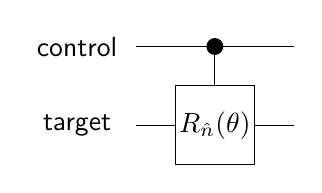
\begin{tikzpicture}[scale=.5] \node[draw=none] at (-3.5, 2) {control}; \node[draw=none] at (-3.5, 0) {target}; \draw (-2, 2) -- (2, 2); \draw[fill=black] (0, 2) circle (.2); \draw (0, 2) -- (0, 1); \draw (-2,0) -- (-1, 0); \draw (1, 0) -- (2, 0); \draw (-1,-1)--(-1,1)--(1,1)--(1,-1)--cycle; \node[draw=none] at (0, 0) {$R_{\hat{n}}(\theta)$}; \end{tikzpicture} } \]


\begin{DoxyParams}[1]{Parameters}
\mbox{\tt in,out}  & {\em multi\+Qubit} & object representing the set of all qubits \\
\hline
\mbox{\tt in}  & {\em control\+Qubit} & qubit with value 1 in the rotated states \\
\hline
\mbox{\tt in}  & {\em target\+Qubit} & qubit to rotate \\
\hline
\mbox{\tt in}  & {\em angle} & angle by which to rotate in radians \\
\hline
\mbox{\tt in}  & {\em axis} & vector around which to rotate (can be non-\/unit; will be normalised) \\
\hline
\end{DoxyParams}

\begin{DoxyExceptions}{Exceptions}
{\em exit\+With\+Error} & if either {\ttfamily control\+Qubit} or {\ttfamily target\+Qubit} are outside \mbox{[}0, {\ttfamily multi\+Qubit.\+num\+Qubits}) or are equal or if {\ttfamily axis} is the zero vector \\
\hline
\end{DoxyExceptions}


Definition at line 122 of file Qu\+E\+S\+T.\+cpp.



References controlled\+Compact\+Unitary(), Complex\+::imag, Complex\+::real, Vector\+::x, Vector\+::y, and Vector\+::z.



Referenced by controlled\+Rotate\+X(), controlled\+Rotate\+Y(), and controlled\+Rotate\+Z().


\begin{DoxyCode}
122                                                                                                            
                         \{
123 
124     \textcolor{keywordtype}{double} mag = sqrt(pow(axis.\mbox{\hyperlink{structVector_aac7abe171ba4bada50ed72acba6259fc}{x}},2) + pow(axis.\mbox{\hyperlink{structVector_a375ca805d4c808a53d7c4e0c737ae3de}{y}},2) + pow(axis.\mbox{\hyperlink{structVector_ad4e863651be7d6b7e2b28cd7445a0ccf}{z}},2));
125     \mbox{\hyperlink{structVector}{Vector}} unitAxis = \{axis.\mbox{\hyperlink{structVector_aac7abe171ba4bada50ed72acba6259fc}{x}}/mag, axis.\mbox{\hyperlink{structVector_a375ca805d4c808a53d7c4e0c737ae3de}{y}}/mag, axis.\mbox{\hyperlink{structVector_ad4e863651be7d6b7e2b28cd7445a0ccf}{z}}/mag\};
126 
127     \mbox{\hyperlink{structComplex}{Complex}} alpha, beta;
128     alpha.\mbox{\hyperlink{structComplex_a479ad939835457595fcca3ca55c06283}{real}} = cos(angle/2.0);
129     alpha.\mbox{\hyperlink{structComplex_a1151948284b21c0052f203f23ab931d9}{imag}} = -sin(angle/2.0)*unitAxis.\mbox{\hyperlink{structVector_ad4e863651be7d6b7e2b28cd7445a0ccf}{z}};    
130     beta.\mbox{\hyperlink{structComplex_a479ad939835457595fcca3ca55c06283}{real}} = sin(angle/2.0)*unitAxis.\mbox{\hyperlink{structVector_a375ca805d4c808a53d7c4e0c737ae3de}{y}};
131     beta.\mbox{\hyperlink{structComplex_a1151948284b21c0052f203f23ab931d9}{imag}} = -sin(angle/2.0)*unitAxis.\mbox{\hyperlink{structVector_aac7abe171ba4bada50ed72acba6259fc}{x}};
132     \mbox{\hyperlink{QuEST_8h_ab4812953bc457405b3aa05a4c2f64f4a}{controlledCompactUnitary}}(multiQubit, controlQubit, targetQubit, alpha, beta);
133 \}
\end{DoxyCode}
\mbox{\Hypertarget{QuEST_8cpp_ac6923ac57e67d9a21096e06f6a9012f6}\label{QuEST_8cpp_ac6923ac57e67d9a21096e06f6a9012f6}} 
\index{Qu\+E\+S\+T.\+cpp@{Qu\+E\+S\+T.\+cpp}!controlled\+RotateX@{controlled\+RotateX}}
\index{controlled\+RotateX@{controlled\+RotateX}!Qu\+E\+S\+T.\+cpp@{Qu\+E\+S\+T.\+cpp}}
\paragraph{\texorpdfstring{controlled\+Rotate\+X()}{controlledRotateX()}}
{\footnotesize\ttfamily void controlled\+RotateX (\begin{DoxyParamCaption}\item[{\mbox{\hyperlink{structMultiQubit}{Multi\+Qubit}}}]{multi\+Qubit,  }\item[{const int}]{control\+Qubit,  }\item[{const int}]{target\+Qubit,  }\item[{\mbox{\hyperlink{QuEST__precision_8h_a4b654506f18b8bfd61ad2a29a7e38c25}{R\+E\+AL}}}]{angle }\end{DoxyParamCaption})}



Applies a controlled rotation by a given angle around the X-\/axis of the Bloch-\/sphere. 

The target qubit is rotated in states where the control qubit has value 1.

\[ \setlength{\fboxrule}{0.01pt} \fbox{ 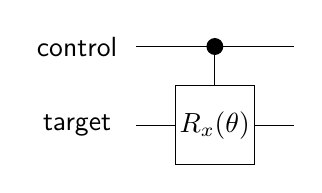
\begin{tikzpicture}[scale=.5] \node[draw=none] at (-3.5, 2) {control}; \node[draw=none] at (-3.5, 0) {target}; \draw (-2, 2) -- (2, 2); \draw[fill=black] (0, 2) circle (.2); \draw (0, 2) -- (0, 1); \draw (-2,0) -- (-1, 0); \draw (1, 0) -- (2, 0); \draw (-1,-1)--(-1,1)--(1,1)--(1,-1)--cycle; \node[draw=none] at (0, 0) {$R_x(\theta)$}; \end{tikzpicture} } \] ~\newline
 
\begin{DoxyParams}[1]{Parameters}
\mbox{\tt in,out}  & {\em multi\+Qubit} & object representing the set of all qubits \\
\hline
\mbox{\tt in}  & {\em control\+Qubit} & qubit which has value 1 in the rotated states \\
\hline
\mbox{\tt in}  & {\em tagret\+Qubit} & qubit to rotate \\
\hline
\mbox{\tt in}  & {\em angle} & angle by which to rotate the target qubit in radians \\
\hline
\end{DoxyParams}

\begin{DoxyExceptions}{Exceptions}
{\em exit\+With\+Error} & if either {\ttfamily control\+Qubit} or {\ttfamily target\+Qubit} are outside \mbox{[}0, {\ttfamily multi\+Qubit.\+num\+Qubits}) or are equal. \\
\hline
\end{DoxyExceptions}


Definition at line 135 of file Qu\+E\+S\+T.\+cpp.



References controlled\+Rotate\+Around\+Axis().


\begin{DoxyCode}
135                                                                                                         \{
136 
137     \mbox{\hyperlink{structVector}{Vector}} unitAxis = \{1, 0, 0\};
138     \mbox{\hyperlink{QuEST_8cpp_ad41f82b41149393a642391b67b3a287e}{controlledRotateAroundAxis}}(multiQubit, controlQubit, targetQubit, angle, 
      unitAxis);
139 \}
\end{DoxyCode}
\mbox{\Hypertarget{QuEST_8cpp_a71e90a2f7292116338c062934f9d1202}\label{QuEST_8cpp_a71e90a2f7292116338c062934f9d1202}} 
\index{Qu\+E\+S\+T.\+cpp@{Qu\+E\+S\+T.\+cpp}!controlled\+RotateY@{controlled\+RotateY}}
\index{controlled\+RotateY@{controlled\+RotateY}!Qu\+E\+S\+T.\+cpp@{Qu\+E\+S\+T.\+cpp}}
\paragraph{\texorpdfstring{controlled\+Rotate\+Y()}{controlledRotateY()}}
{\footnotesize\ttfamily void controlled\+RotateY (\begin{DoxyParamCaption}\item[{\mbox{\hyperlink{structMultiQubit}{Multi\+Qubit}}}]{multi\+Qubit,  }\item[{const int}]{control\+Qubit,  }\item[{const int}]{target\+Qubit,  }\item[{\mbox{\hyperlink{QuEST__precision_8h_a4b654506f18b8bfd61ad2a29a7e38c25}{R\+E\+AL}}}]{angle }\end{DoxyParamCaption})}



Applies a controlled rotation by a given angle around the Y-\/axis of the Bloch-\/sphere. 

The target qubit is rotated in states where the control qubit has value 1.

\[ \setlength{\fboxrule}{0.01pt} \fbox{ 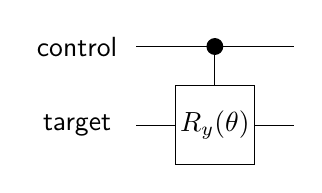
\begin{tikzpicture}[scale=.5] \node[draw=none] at (-3.5, 2) {control}; \node[draw=none] at (-3.5, 0) {target}; \draw (-2, 2) -- (2, 2); \draw[fill=black] (0, 2) circle (.2); \draw (0, 2) -- (0, 1); \draw (-2,0) -- (-1, 0); \draw (1, 0) -- (2, 0); \draw (-1,-1)--(-1,1)--(1,1)--(1,-1)--cycle; \node[draw=none] at (0, 0) {$R_y(\theta)$}; \end{tikzpicture} } \] ~\newline
 
\begin{DoxyParams}[1]{Parameters}
\mbox{\tt in,out}  & {\em multi\+Qubit} & object representing the set of all qubits \\
\hline
\mbox{\tt in}  & {\em control\+Qubit} & qubit which has value 1 in the rotated states \\
\hline
\mbox{\tt in}  & {\em tagret\+Qubit} & qubit to rotate \\
\hline
\mbox{\tt in}  & {\em angle} & angle by which to rotate the target qubit in radians \\
\hline
\end{DoxyParams}

\begin{DoxyExceptions}{Exceptions}
{\em exit\+With\+Error} & if either {\ttfamily control\+Qubit} or {\ttfamily target\+Qubit} are outside \mbox{[}0, {\ttfamily multi\+Qubit.\+num\+Qubits}) or are equal. \\
\hline
\end{DoxyExceptions}


Definition at line 141 of file Qu\+E\+S\+T.\+cpp.



References controlled\+Rotate\+Around\+Axis().


\begin{DoxyCode}
141                                                                                                         \{
142 
143     \mbox{\hyperlink{structVector}{Vector}} unitAxis = \{0, 1, 0\};
144     \mbox{\hyperlink{QuEST_8cpp_ad41f82b41149393a642391b67b3a287e}{controlledRotateAroundAxis}}(multiQubit, controlQubit, targetQubit, angle, 
      unitAxis);
145 \}
\end{DoxyCode}
\mbox{\Hypertarget{QuEST_8cpp_a668e5d2634b02e98bc73675ccb11d61c}\label{QuEST_8cpp_a668e5d2634b02e98bc73675ccb11d61c}} 
\index{Qu\+E\+S\+T.\+cpp@{Qu\+E\+S\+T.\+cpp}!controlled\+RotateZ@{controlled\+RotateZ}}
\index{controlled\+RotateZ@{controlled\+RotateZ}!Qu\+E\+S\+T.\+cpp@{Qu\+E\+S\+T.\+cpp}}
\paragraph{\texorpdfstring{controlled\+Rotate\+Z()}{controlledRotateZ()}}
{\footnotesize\ttfamily void controlled\+RotateZ (\begin{DoxyParamCaption}\item[{\mbox{\hyperlink{structMultiQubit}{Multi\+Qubit}}}]{multi\+Qubit,  }\item[{const int}]{control\+Qubit,  }\item[{const int}]{target\+Qubit,  }\item[{\mbox{\hyperlink{QuEST__precision_8h_a4b654506f18b8bfd61ad2a29a7e38c25}{R\+E\+AL}}}]{angle }\end{DoxyParamCaption})}



Applies a controlled rotation by a given angle around the Z-\/axis of the Bloch-\/sphere. 

The target qubit is rotated in states where the control qubit has value 1.

\[ \setlength{\fboxrule}{0.01pt} \fbox{ 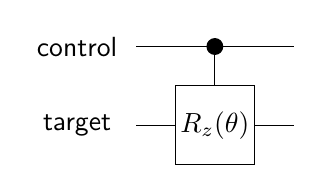
\begin{tikzpicture}[scale=.5] \node[draw=none] at (-3.5, 2) {control}; \node[draw=none] at (-3.5, 0) {target}; \draw (-2, 2) -- (2, 2); \draw[fill=black] (0, 2) circle (.2); \draw (0, 2) -- (0, 1); \draw (-2,0) -- (-1, 0); \draw (1, 0) -- (2, 0); \draw (-1,-1)--(-1,1)--(1,1)--(1,-1)--cycle; \node[draw=none] at (0, 0) {$R_z(\theta)$}; \end{tikzpicture} } \] ~\newline
 
\begin{DoxyParams}[1]{Parameters}
\mbox{\tt in,out}  & {\em multi\+Qubit} & object representing the set of all qubits \\
\hline
\mbox{\tt in}  & {\em control\+Qubit} & qubit which has value 1 in the rotated states \\
\hline
\mbox{\tt in}  & {\em tagret\+Qubit} & qubit to rotate \\
\hline
\mbox{\tt in}  & {\em angle} & angle by which to rotate the target qubit in radians \\
\hline
\end{DoxyParams}

\begin{DoxyExceptions}{Exceptions}
{\em exit\+With\+Error} & if either {\ttfamily control\+Qubit} or {\ttfamily target\+Qubit} are outside \mbox{[}0, {\ttfamily multi\+Qubit.\+num\+Qubits}) or are equal. \\
\hline
\end{DoxyExceptions}


Definition at line 147 of file Qu\+E\+S\+T.\+cpp.



References controlled\+Rotate\+Around\+Axis().


\begin{DoxyCode}
147                                                                                                         \{
148 
149     \mbox{\hyperlink{structVector}{Vector}} unitAxis = \{0, 0, 1\};
150     \mbox{\hyperlink{QuEST_8cpp_ad41f82b41149393a642391b67b3a287e}{controlledRotateAroundAxis}}(multiQubit, controlQubit, targetQubit, angle, 
      unitAxis);
151 \}
\end{DoxyCode}
\mbox{\Hypertarget{QuEST_8cpp_ab76254cfde16f0808476649507a1a2fc}\label{QuEST_8cpp_ab76254cfde16f0808476649507a1a2fc}} 
\index{Qu\+E\+S\+T.\+cpp@{Qu\+E\+S\+T.\+cpp}!hash\+String@{hash\+String}}
\index{hash\+String@{hash\+String}!Qu\+E\+S\+T.\+cpp@{Qu\+E\+S\+T.\+cpp}}
\paragraph{\texorpdfstring{hash\+String()}{hashString()}}
{\footnotesize\ttfamily unsigned long int hash\+String (\begin{DoxyParamCaption}\item[{char $\ast$}]{str }\end{DoxyParamCaption})}



Definition at line 238 of file Qu\+E\+S\+T.\+cpp.



Referenced by Qu\+E\+S\+T\+Seed\+Random\+Default().


\begin{DoxyCode}
238                                        \{
239     \textcolor{keywordtype}{unsigned} \textcolor{keywordtype}{long} \textcolor{keywordtype}{int} hash = 5381;
240     \textcolor{keywordtype}{int} c;
241 
242     \textcolor{keywordflow}{while} ((c = *str++))
243         hash = ((hash << 5) + hash) + c; \textcolor{comment}{/* hash * 33 + c */}
244 
245     \textcolor{keywordflow}{return} hash;    
246 \}
\end{DoxyCode}
\mbox{\Hypertarget{QuEST_8cpp_aedb5ef39da69e7895d714980dc621261}\label{QuEST_8cpp_aedb5ef39da69e7895d714980dc621261}} 
\index{Qu\+E\+S\+T.\+cpp@{Qu\+E\+S\+T.\+cpp}!Qu\+E\+S\+T\+Seed\+Random@{Qu\+E\+S\+T\+Seed\+Random}}
\index{Qu\+E\+S\+T\+Seed\+Random@{Qu\+E\+S\+T\+Seed\+Random}!Qu\+E\+S\+T.\+cpp@{Qu\+E\+S\+T.\+cpp}}
\paragraph{\texorpdfstring{Qu\+E\+S\+T\+Seed\+Random()}{QuESTSeedRandom()}}
{\footnotesize\ttfamily void Qu\+E\+S\+T\+Seed\+Random (\begin{DoxyParamCaption}\item[{unsigned long int $\ast$}]{seed\+Array,  }\item[{int}]{num\+Seeds }\end{DoxyParamCaption})}



num\+Seeds $<$= 64 

Seed the Mersenne Twister used for random number generation in the Qu\+E\+ST environment with a user defined seed. 

Definition at line 231 of file Qu\+E\+S\+T.\+cpp.



References init\+\_\+by\+\_\+array().


\begin{DoxyCode}
231                                                                 \{
232     \textcolor{comment}{// init MT random number generator with user defined list of seeds}
233     \textcolor{comment}{// for the MPI version, it is ok that all procs will get the same seed as random numbers will only be }
234     \textcolor{comment}{// used by the master process}
235     \mbox{\hyperlink{mt19937ar_8cpp_ac1283f9b1ed571332f5ffe53545ffc16}{init\_by\_array}}(seedArray, numSeeds); 
236 \}
\end{DoxyCode}
\mbox{\Hypertarget{QuEST_8cpp_a30b2a5228b8a21419db8aa82fa5e3167}\label{QuEST_8cpp_a30b2a5228b8a21419db8aa82fa5e3167}} 
\index{Qu\+E\+S\+T.\+cpp@{Qu\+E\+S\+T.\+cpp}!Qu\+E\+S\+T\+Seed\+Random\+Default@{Qu\+E\+S\+T\+Seed\+Random\+Default}}
\index{Qu\+E\+S\+T\+Seed\+Random\+Default@{Qu\+E\+S\+T\+Seed\+Random\+Default}!Qu\+E\+S\+T.\+cpp@{Qu\+E\+S\+T.\+cpp}}
\paragraph{\texorpdfstring{Qu\+E\+S\+T\+Seed\+Random\+Default()}{QuESTSeedRandomDefault()}}
{\footnotesize\ttfamily void Qu\+E\+S\+T\+Seed\+Random\+Default (\begin{DoxyParamCaption}\item[{void}]{ }\end{DoxyParamCaption})}



Seed the Mersenne Twister used for random number generation in the Qu\+E\+ST environment with an example defualt seed. 

This default seeding function uses the mt19937 init\+\_\+by\+\_\+array function with three keys -- time, pid and hostname. Subsequent calls to mt19937 genrand functions will use this seeding. For a multi process code, the same seed is given to all process, therefore this seeding is only appropriate to use for functions such as measure where all processes require the same random value.

For more information about the MT, see \href{http://www.math.sci.hiroshima-u.ac.jp/~m-mat/MT/MT2002/emt19937ar.html}{\tt http\+://www.\+math.\+sci.\+hiroshima-\/u.\+ac.\+jp/$\sim$m-\/mat/\+M\+T/\+M\+T2002/emt19937ar.\+html} 

Definition at line 206 of file Qu\+E\+S\+T.\+cpp.



References hash\+String(), and init\+\_\+by\+\_\+array().


\begin{DoxyCode}
206                              \{
207     \textcolor{comment}{// init MT random number generator with three keys -- time, pid and a hash of hostname }
208     \textcolor{comment}{// for the MPI version, it is ok that all procs will get the same seed as random numbers will only be }
209     \textcolor{comment}{// used by the master process}
210 
211     \textcolor{keyword}{struct }timeval  tv;
212     gettimeofday(&tv, NULL);
213 
214     \textcolor{keywordtype}{double} time\_in\_mill = 
215         (tv.tv\_sec) * 1000 + (tv.tv\_usec) / 1000 ; \textcolor{comment}{// convert tv\_sec & tv\_usec to millisecond}
216 
217     \textcolor{keywordtype}{unsigned} \textcolor{keywordtype}{long} \textcolor{keywordtype}{int} pid = getpid();
218     \textcolor{keywordtype}{unsigned} \textcolor{keywordtype}{long} \textcolor{keywordtype}{int} msecs = (\textcolor{keywordtype}{unsigned} \textcolor{keywordtype}{long} int) time\_in\_mill;
219     \textcolor{keywordtype}{char} hostName[MAXHOSTNAMELEN+1];
220     gethostname(hostName, \textcolor{keyword}{sizeof}(hostName));
221     \textcolor{keywordtype}{unsigned} \textcolor{keywordtype}{long} \textcolor{keywordtype}{int} hostNameInt = \mbox{\hyperlink{QuEST_8cpp_ab76254cfde16f0808476649507a1a2fc}{hashString}}(hostName);
222 
223     \textcolor{keywordtype}{unsigned} \textcolor{keywordtype}{long} \textcolor{keywordtype}{int} key[3];
224     key[0] = msecs; key[1] = pid; key[2] = hostNameInt;
225     \mbox{\hyperlink{mt19937ar_8cpp_ac1283f9b1ed571332f5ffe53545ffc16}{init\_by\_array}}(key, 3); 
226 \}
\end{DoxyCode}
\mbox{\Hypertarget{QuEST_8cpp_aa5e77e0e64f3a4a3d3f5cc7382bffcd9}\label{QuEST_8cpp_aa5e77e0e64f3a4a3d3f5cc7382bffcd9}} 
\index{Qu\+E\+S\+T.\+cpp@{Qu\+E\+S\+T.\+cpp}!report\+Multi\+Qubit\+Params@{report\+Multi\+Qubit\+Params}}
\index{report\+Multi\+Qubit\+Params@{report\+Multi\+Qubit\+Params}!Qu\+E\+S\+T.\+cpp@{Qu\+E\+S\+T.\+cpp}}
\paragraph{\texorpdfstring{report\+Multi\+Qubit\+Params()}{reportMultiQubitParams()}}
{\footnotesize\ttfamily void report\+Multi\+Qubit\+Params (\begin{DoxyParamCaption}\item[{\mbox{\hyperlink{structMultiQubit}{Multi\+Qubit}}}]{multi\+Qubit }\end{DoxyParamCaption})}



Report metainformation about a set of qubits\+: number of qubits, number of probability amplitudes. 


\begin{DoxyParams}[1]{Parameters}
\mbox{\tt in,out}  & {\em multi\+Qubit} & object representing the set of qubits \\
\hline
\mbox{\tt in}  & {\em env} & object representing the execution environment (local, multinode etc) \\
\hline
\end{DoxyParams}


Definition at line 80 of file Qu\+E\+S\+T.\+cpp.



References Multi\+Qubit\+::chunk\+Id, Multi\+Qubit\+::num\+Chunks, and Multi\+Qubit\+::num\+Qubits.


\begin{DoxyCode}
80                                                   \{
81         \textcolor{keywordtype}{long} \textcolor{keywordtype}{long} \textcolor{keywordtype}{int} numAmps = 1L << multiQubit.\mbox{\hyperlink{structMultiQubit_ab5b9795bdc6fb5855e1974dcbbaeb36f}{numQubits}};
82         \textcolor{keywordtype}{long} \textcolor{keywordtype}{long} \textcolor{keywordtype}{int} numAmpsPerRank = numAmps/multiQubit.\mbox{\hyperlink{structMultiQubit_acd43f2f57991709c9e94f73662c972b2}{numChunks}};
83         \textcolor{keywordflow}{if} (multiQubit.\mbox{\hyperlink{structMultiQubit_ab10c88249fa3825d6227ceec01d37e37}{chunkId}}==0)\{
84                 printf(\textcolor{stringliteral}{"QUBITS:\(\backslash\)n"});
85                 printf(\textcolor{stringliteral}{"Number of qubits is %d.\(\backslash\)n"}, multiQubit.\mbox{\hyperlink{structMultiQubit_ab5b9795bdc6fb5855e1974dcbbaeb36f}{numQubits}});
86                 printf(\textcolor{stringliteral}{"Number of amps is %lld.\(\backslash\)n"}, numAmps);
87                 printf(\textcolor{stringliteral}{"Number of amps per rank is %lld.\(\backslash\)n"}, numAmpsPerRank);
88     \}
89 \}
\end{DoxyCode}
\mbox{\Hypertarget{QuEST_8cpp_a96f4de9ce7fefc7680a44d601fc3d894}\label{QuEST_8cpp_a96f4de9ce7fefc7680a44d601fc3d894}} 
\index{Qu\+E\+S\+T.\+cpp@{Qu\+E\+S\+T.\+cpp}!report\+State@{report\+State}}
\index{report\+State@{report\+State}!Qu\+E\+S\+T.\+cpp@{Qu\+E\+S\+T.\+cpp}}
\paragraph{\texorpdfstring{report\+State()}{reportState()}}
{\footnotesize\ttfamily void report\+State (\begin{DoxyParamCaption}\item[{\mbox{\hyperlink{structMultiQubit}{Multi\+Qubit}}}]{multi\+Qubit }\end{DoxyParamCaption})}



Print the current state vector of probability amplitudes for a set of qubits to file. 

File format\+: \begin{DoxyVerb}real, imag
realComponent1, imagComponent1
realComponent2, imagComponent2
...
realComponentN, imagComponentN
\end{DoxyVerb}


File naming convention\+:

For each node that the program runs on, a file \textquotesingle{}state\+\_\+rank\+\_\+\mbox{[}node\+\_\+rank\mbox{]}.csv\textquotesingle{} is generated. If there is more than one node, ranks after the first do not include the header \begin{DoxyVerb}real, imag
\end{DoxyVerb}
 so that files are easier to combine. 
\begin{DoxyParams}[1]{Parameters}
\mbox{\tt in,out}  & {\em multi\+Qubit} & object representing the set of qubits \\
\hline
\end{DoxyParams}


Definition at line 62 of file Qu\+E\+S\+T.\+cpp.



References Multi\+Qubit\+::chunk\+Id, Complex\+Array\+::imag, Multi\+Qubit\+::num\+Amps, Complex\+Array\+::real, and Multi\+Qubit\+::state\+Vec.


\begin{DoxyCode}
62                                        \{
63         FILE *state;
64         \textcolor{keywordtype}{char} filename[100];
65         \textcolor{keywordtype}{long} \textcolor{keywordtype}{long} \textcolor{keywordtype}{int} index;
66         sprintf(filename, \textcolor{stringliteral}{"state\_rank\_%d.csv"}, multiQubit.\mbox{\hyperlink{structMultiQubit_ab10c88249fa3825d6227ceec01d37e37}{chunkId}});
67         state = fopen(filename, \textcolor{stringliteral}{"w"});
68         \textcolor{keywordflow}{if} (multiQubit.\mbox{\hyperlink{structMultiQubit_ab10c88249fa3825d6227ceec01d37e37}{chunkId}}==0) fprintf(state, \textcolor{stringliteral}{"real, imag\(\backslash\)n"});
69 
70         \textcolor{keywordflow}{for}(index=0; index<multiQubit.\mbox{\hyperlink{structMultiQubit_ae16f47d8b725c914fb7f66b6498d79db}{numAmps}}; index++)\{
71                 fprintf(state, \textcolor{stringliteral}{"%.12f, %.12f\(\backslash\)n"}, multiQubit.\mbox{\hyperlink{structMultiQubit_a45483190d6b01ef6b2f98f2bec9ab94f}{stateVec}}.
      \mbox{\hyperlink{structComplexArray_a4195cac6c784ea1b6271f1c7dba1548a}{real}}[index], multiQubit.\mbox{\hyperlink{structMultiQubit_a45483190d6b01ef6b2f98f2bec9ab94f}{stateVec}}.\mbox{\hyperlink{structComplexArray_a79dde47c7ae530c79cebfdf57b225968}{imag}}[index]);
72         \}
73         fclose(state);
74 \}
\end{DoxyCode}
\mbox{\Hypertarget{QuEST_8cpp_a8810423457803005fecd415f4299f40d}\label{QuEST_8cpp_a8810423457803005fecd415f4299f40d}} 
\index{Qu\+E\+S\+T.\+cpp@{Qu\+E\+S\+T.\+cpp}!rotate\+Around\+Axis@{rotate\+Around\+Axis}}
\index{rotate\+Around\+Axis@{rotate\+Around\+Axis}!Qu\+E\+S\+T.\+cpp@{Qu\+E\+S\+T.\+cpp}}
\paragraph{\texorpdfstring{rotate\+Around\+Axis()}{rotateAroundAxis()}}
{\footnotesize\ttfamily void rotate\+Around\+Axis (\begin{DoxyParamCaption}\item[{\mbox{\hyperlink{structMultiQubit}{Multi\+Qubit}}}]{multi\+Qubit,  }\item[{const int}]{rot\+Qubit,  }\item[{\mbox{\hyperlink{QuEST__precision_8h_a4b654506f18b8bfd61ad2a29a7e38c25}{R\+E\+AL}}}]{angle,  }\item[{\mbox{\hyperlink{structVector}{Vector}}}]{unit\+Axis }\end{DoxyParamCaption})}



Rotate a single qubit by a given angle around a given vector on the Bloch-\/sphere. 


\begin{DoxyItemize}
\item The vector must not be zero (else an error is thrown), but needn\textquotesingle{}t be unit magnitude.
\end{DoxyItemize}


\begin{DoxyParams}[1]{Parameters}
\mbox{\tt in,out}  & {\em multi\+Qubit} & object representing the set of all qubits \\
\hline
\mbox{\tt in}  & {\em rot\+Qubit} & qubit to rotate \\
\hline
\mbox{\tt in}  & {\em angle} & angle by which to rotate in radians \\
\hline
\mbox{\tt in}  & {\em axis} & vector around which to rotate \\
\hline
\end{DoxyParams}

\begin{DoxyExceptions}{Exceptions}
{\em exit\+With\+Error} & if {\ttfamily rot\+Qubit} is outside \mbox{[}0, {\ttfamily multi\+Qubit.\+num\+Qubits}), or if {\ttfamily axis} is the zero vector \\
\hline
\end{DoxyExceptions}


Definition at line 91 of file Qu\+E\+S\+T.\+cpp.



References compact\+Unitary(), Complex\+::imag, Complex\+::real, Vector\+::x, Vector\+::y, and Vector\+::z.



Referenced by rotate\+X(), rotate\+Y(), and rotate\+Z().


\begin{DoxyCode}
91                                                                                          \{
92 
93     \textcolor{keywordtype}{double} mag = sqrt(pow(axis.\mbox{\hyperlink{structVector_aac7abe171ba4bada50ed72acba6259fc}{x}},2) + pow(axis.\mbox{\hyperlink{structVector_a375ca805d4c808a53d7c4e0c737ae3de}{y}},2) + pow(axis.\mbox{\hyperlink{structVector_ad4e863651be7d6b7e2b28cd7445a0ccf}{z}},2));
94     \mbox{\hyperlink{structVector}{Vector}} unitAxis = \{axis.\mbox{\hyperlink{structVector_aac7abe171ba4bada50ed72acba6259fc}{x}}/mag, axis.\mbox{\hyperlink{structVector_a375ca805d4c808a53d7c4e0c737ae3de}{y}}/mag, axis.\mbox{\hyperlink{structVector_ad4e863651be7d6b7e2b28cd7445a0ccf}{z}}/mag\};
95 
96     \mbox{\hyperlink{structComplex}{Complex}} alpha, beta;
97     alpha.\mbox{\hyperlink{structComplex_a479ad939835457595fcca3ca55c06283}{real}} = cos(angle/2.0);
98     alpha.\mbox{\hyperlink{structComplex_a1151948284b21c0052f203f23ab931d9}{imag}} = -sin(angle/2.0)*unitAxis.\mbox{\hyperlink{structVector_ad4e863651be7d6b7e2b28cd7445a0ccf}{z}};    
99     beta.\mbox{\hyperlink{structComplex_a479ad939835457595fcca3ca55c06283}{real}} = sin(angle/2.0)*unitAxis.\mbox{\hyperlink{structVector_a375ca805d4c808a53d7c4e0c737ae3de}{y}};
100     beta.\mbox{\hyperlink{structComplex_a1151948284b21c0052f203f23ab931d9}{imag}} = -sin(angle/2.0)*unitAxis.\mbox{\hyperlink{structVector_aac7abe171ba4bada50ed72acba6259fc}{x}};
101     \mbox{\hyperlink{QuEST_8h_ad13ae1902276195d0df106116e032aff}{compactUnitary}}(multiQubit, rotQubit, alpha, beta);
102 \}
\end{DoxyCode}
\mbox{\Hypertarget{QuEST_8cpp_a6cc7fa705a2f2e6b486b49c5589d5df5}\label{QuEST_8cpp_a6cc7fa705a2f2e6b486b49c5589d5df5}} 
\index{Qu\+E\+S\+T.\+cpp@{Qu\+E\+S\+T.\+cpp}!rotateX@{rotateX}}
\index{rotateX@{rotateX}!Qu\+E\+S\+T.\+cpp@{Qu\+E\+S\+T.\+cpp}}
\paragraph{\texorpdfstring{rotate\+X()}{rotateX()}}
{\footnotesize\ttfamily void rotateX (\begin{DoxyParamCaption}\item[{\mbox{\hyperlink{structMultiQubit}{Multi\+Qubit}}}]{multi\+Qubit,  }\item[{const int}]{rot\+Qubit,  }\item[{\mbox{\hyperlink{QuEST__precision_8h_a4b654506f18b8bfd61ad2a29a7e38c25}{R\+E\+AL}}}]{angle }\end{DoxyParamCaption})}



Rotate a single qubit by a given angle around the X-\/axis of the Bloch-\/sphere. 

For angle $\theta$, applies \[ \begin{pmatrix} \cos\theta/2 & -i \sin \theta/2\\ -i \sin \theta/2 & \cos \theta/2 \end{pmatrix} \]

\[ \setlength{\fboxrule}{0.01pt} \fbox{ 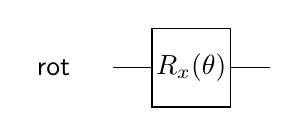
\begin{tikzpicture}[scale=.5] \node[draw=none] at (-3.5, 0) {rot}; \draw (-2,0) -- (-1, 0); \draw (1, 0) -- (2, 0); \draw (-1,-1)--(-1,1)--(1,1)--(1,-1)--cycle; \node[draw=none] at (0, 0) {$R_x(\theta)$}; \end{tikzpicture} } \]


\begin{DoxyParams}[1]{Parameters}
\mbox{\tt in,out}  & {\em multi\+Qubit} & object representing the set of all qubits \\
\hline
\mbox{\tt in}  & {\em rot\+Qubit} & qubit to rotate \\
\hline
\mbox{\tt in}  & {\em angle} & angle by which to rotate in radians \\
\hline
\end{DoxyParams}

\begin{DoxyExceptions}{Exceptions}
{\em exit\+With\+Error} & if {\ttfamily rot\+Qubit} is outside \mbox{[}0, {\ttfamily multi\+Qubit.\+num\+Qubits}). \\
\hline
\end{DoxyExceptions}


Definition at line 104 of file Qu\+E\+S\+T.\+cpp.



References rotate\+Around\+Axis().


\begin{DoxyCode}
104                                                                    \{
105 
106     \mbox{\hyperlink{structVector}{Vector}} unitAxis = \{1, 0, 0\};
107     \mbox{\hyperlink{QuEST_8cpp_a8810423457803005fecd415f4299f40d}{rotateAroundAxis}}(multiQubit, rotQubit, angle, unitAxis);
108 \}
\end{DoxyCode}
\mbox{\Hypertarget{QuEST_8cpp_ace0d3592d38a990e81a434c4e9681500}\label{QuEST_8cpp_ace0d3592d38a990e81a434c4e9681500}} 
\index{Qu\+E\+S\+T.\+cpp@{Qu\+E\+S\+T.\+cpp}!rotateY@{rotateY}}
\index{rotateY@{rotateY}!Qu\+E\+S\+T.\+cpp@{Qu\+E\+S\+T.\+cpp}}
\paragraph{\texorpdfstring{rotate\+Y()}{rotateY()}}
{\footnotesize\ttfamily void rotateY (\begin{DoxyParamCaption}\item[{\mbox{\hyperlink{structMultiQubit}{Multi\+Qubit}}}]{multi\+Qubit,  }\item[{const int}]{rot\+Qubit,  }\item[{\mbox{\hyperlink{QuEST__precision_8h_a4b654506f18b8bfd61ad2a29a7e38c25}{R\+E\+AL}}}]{angle }\end{DoxyParamCaption})}



Rotate a single qubit by a given angle around the Y-\/axis of the Bloch-\/sphere. 

For angle $\theta$, applies \[ \begin{pmatrix} \cos\theta/2 & \sin \theta/2\\ \sin \theta/2 & \cos \theta/2 \end{pmatrix} \] ~\newline
 \[ \setlength{\fboxrule}{0.01pt} \fbox{ 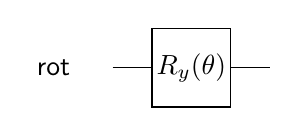
\begin{tikzpicture}[scale=.5] \node[draw=none] at (-3.5, 0) {rot}; \draw (-2,0) -- (-1, 0); \draw (1, 0) -- (2, 0); \draw (-1,-1)--(-1,1)--(1,1)--(1,-1)--cycle; \node[draw=none] at (0, 0) {$R_y(\theta)$}; \end{tikzpicture} } \]


\begin{DoxyParams}[1]{Parameters}
\mbox{\tt in,out}  & {\em multi\+Qubit} & object representing the set of all qubits \\
\hline
\mbox{\tt in}  & {\em rot\+Qubit} & qubit to rotate \\
\hline
\mbox{\tt in}  & {\em angle} & angle by which to rotate in radians \\
\hline
\end{DoxyParams}

\begin{DoxyExceptions}{Exceptions}
{\em exit\+With\+Error} & if {\ttfamily rot\+Qubit} is outside \mbox{[}0, {\ttfamily multi\+Qubit.\+num\+Qubits}). \\
\hline
\end{DoxyExceptions}


Definition at line 110 of file Qu\+E\+S\+T.\+cpp.



References rotate\+Around\+Axis().


\begin{DoxyCode}
110                                                                    \{
111 
112     \mbox{\hyperlink{structVector}{Vector}} unitAxis = \{0, 1, 0\};
113     \mbox{\hyperlink{QuEST_8cpp_a8810423457803005fecd415f4299f40d}{rotateAroundAxis}}(multiQubit, rotQubit, angle, unitAxis);
114 \}
\end{DoxyCode}
\mbox{\Hypertarget{QuEST_8cpp_abd621412ad30c1b034f4ce153c4afe10}\label{QuEST_8cpp_abd621412ad30c1b034f4ce153c4afe10}} 
\index{Qu\+E\+S\+T.\+cpp@{Qu\+E\+S\+T.\+cpp}!rotateZ@{rotateZ}}
\index{rotateZ@{rotateZ}!Qu\+E\+S\+T.\+cpp@{Qu\+E\+S\+T.\+cpp}}
\paragraph{\texorpdfstring{rotate\+Z()}{rotateZ()}}
{\footnotesize\ttfamily void rotateZ (\begin{DoxyParamCaption}\item[{\mbox{\hyperlink{structMultiQubit}{Multi\+Qubit}}}]{multi\+Qubit,  }\item[{const int}]{rot\+Qubit,  }\item[{\mbox{\hyperlink{QuEST__precision_8h_a4b654506f18b8bfd61ad2a29a7e38c25}{R\+E\+AL}}}]{angle }\end{DoxyParamCaption})}



Rotate a single qubit by a given angle around the Z-\/axis of the Bloch-\/sphere (also known as a phase shift gate). 

For angle $\theta$, applies \[ \begin{pmatrix} \exp(-i \theta/2) & 0 \\ 0 & \exp(i \theta/2) \end{pmatrix} \]

\[ \setlength{\fboxrule}{0.01pt} \fbox{ 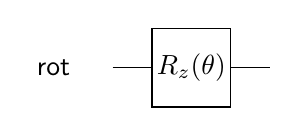
\begin{tikzpicture}[scale=.5] \node[draw=none] at (-3.5, 0) {rot}; \draw (-2,0) -- (-1, 0); \draw (1, 0) -- (2, 0); \draw (-1,-1)--(-1,1)--(1,1)--(1,-1)--cycle; \node[draw=none] at (0, 0) {$R_z(\theta)$}; \end{tikzpicture} } \]


\begin{DoxyParams}[1]{Parameters}
\mbox{\tt in,out}  & {\em multi\+Qubit} & object representing the set of all qubits \\
\hline
\mbox{\tt in}  & {\em rot\+Qubit} & qubit to rotate \\
\hline
\mbox{\tt in}  & {\em angle} & angle by which to rotate in radians \\
\hline
\end{DoxyParams}

\begin{DoxyExceptions}{Exceptions}
{\em exit\+With\+Error} & if {\ttfamily rot\+Qubit} is outside \mbox{[}0, {\ttfamily multi\+Qubit.\+num\+Qubits}). \\
\hline
\end{DoxyExceptions}


Definition at line 116 of file Qu\+E\+S\+T.\+cpp.



References rotate\+Around\+Axis().


\begin{DoxyCode}
116                                                                    \{
117 
118     \mbox{\hyperlink{structVector}{Vector}} unitAxis = \{0, 0, 1\};
119     \mbox{\hyperlink{QuEST_8cpp_a8810423457803005fecd415f4299f40d}{rotateAroundAxis}}(multiQubit, rotQubit, angle, unitAxis);
120 \}
\end{DoxyCode}
\mbox{\Hypertarget{QuEST_8cpp_adda6c47876a7676488ed0565a19eaa65}\label{QuEST_8cpp_adda6c47876a7676488ed0565a19eaa65}} 
\index{Qu\+E\+S\+T.\+cpp@{Qu\+E\+S\+T.\+cpp}!s\+Gate@{s\+Gate}}
\index{s\+Gate@{s\+Gate}!Qu\+E\+S\+T.\+cpp@{Qu\+E\+S\+T.\+cpp}}
\paragraph{\texorpdfstring{s\+Gate()}{sGate()}}
{\footnotesize\ttfamily void s\+Gate (\begin{DoxyParamCaption}\item[{\mbox{\hyperlink{structMultiQubit}{Multi\+Qubit}}}]{multi\+Qubit,  }\item[{const int}]{target\+Qubit }\end{DoxyParamCaption})}



Apply the single-\/qubit S gate. 

This is a rotation of $\pi/2$ around the Z-\/axis on the Bloch sphere, or the unitary\+: \[ \begin{pmatrix} 1 & 0 \\ 0 & i \end{pmatrix} \]

\[ \setlength{\fboxrule}{0.01pt} \fbox{ 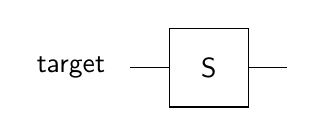
\begin{tikzpicture}[scale=.5] \node[draw=none] at (-3.5, 0) {target}; \draw (-2,0) -- (-1, 0); \draw (1, 0) -- (2, 0); \draw (-1,-1)--(-1,1)--(1,1)--(1,-1)--cycle; \node[draw=none] at (0, 0) {S}; \end{tikzpicture} } \]


\begin{DoxyParams}[1]{Parameters}
\mbox{\tt in,out}  & {\em multi\+Qubit} & object representing the set of all qubits \\
\hline
\mbox{\tt in}  & {\em target\+Qubit} & qubit to operate upon \\
\hline
\end{DoxyParams}

\begin{DoxyExceptions}{Exceptions}
{\em exit\+With\+Error} & if {\ttfamily target\+Qubit} is outside \mbox{[}0, {\ttfamily multi\+Qubit.\+num\+Qubits}) \\
\hline
\end{DoxyExceptions}


Definition at line 158 of file Qu\+E\+S\+T.\+cpp.



References phase\+Gate(), and S\+\_\+\+G\+A\+TE.


\begin{DoxyCode}
159 \{
160     \mbox{\hyperlink{QuEST__internal_8h_aae7a8a7f1ccbddb7f76b6c52b746bb43}{phaseGate}}(multiQubit, targetQubit, \mbox{\hyperlink{QuEST_8h_a5739021c733cecc49647956b2f7338eaa06e60f80fa80cce271793d6d31bcc21f}{S\_GATE}});
161 \} 
\end{DoxyCode}
\mbox{\Hypertarget{QuEST_8cpp_aebaab86326779de55d335cfea3efde8f}\label{QuEST_8cpp_aebaab86326779de55d335cfea3efde8f}} 
\index{Qu\+E\+S\+T.\+cpp@{Qu\+E\+S\+T.\+cpp}!sigmaZ@{sigmaZ}}
\index{sigmaZ@{sigmaZ}!Qu\+E\+S\+T.\+cpp@{Qu\+E\+S\+T.\+cpp}}
\paragraph{\texorpdfstring{sigma\+Z()}{sigmaZ()}}
{\footnotesize\ttfamily void sigmaZ (\begin{DoxyParamCaption}\item[{\mbox{\hyperlink{structMultiQubit}{Multi\+Qubit}}}]{multi\+Qubit,  }\item[{const int}]{target\+Qubit }\end{DoxyParamCaption})}



Apply the single-\/qubit sigma-\/Z (also known as the Z, Pauli-\/Z or phase-\/flip) gate. 

This is a rotation of $\pi$ around the Z-\/axis (a phase shift) on the Bloch sphere. I.\+e. \[ \begin{pmatrix} 1 & 0 \\ 0 & -1 \end{pmatrix} \] ~\newline
 \[ \setlength{\fboxrule}{0.01pt} \fbox{ 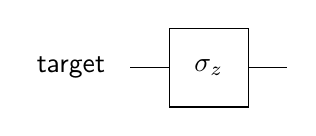
\begin{tikzpicture}[scale=.5] \node[draw=none] at (-3.5, 0) {target}; \draw (-2,0) -- (-1, 0); \draw (1, 0) -- (2, 0); \draw (-1,-1)--(-1,1)--(1,1)--(1,-1)--cycle; \node[draw=none] at (0, 0) {$\sigma_z$}; \end{tikzpicture} } \] ~\newline
 
\begin{DoxyParams}[1]{Parameters}
\mbox{\tt in,out}  & {\em multi\+Qubit} & object representing the set of all qubits \\
\hline
\mbox{\tt in}  & {\em target\+Qubit} & qubit to operate on \\
\hline
\end{DoxyParams}

\begin{DoxyExceptions}{Exceptions}
{\em exit\+With\+Error} & if {\ttfamily target\+Qubit} is outside \mbox{[}0, {\ttfamily multi\+Qubit.\+num\+Qubits}). \\
\hline
\end{DoxyExceptions}


Definition at line 153 of file Qu\+E\+S\+T.\+cpp.



References phase\+Gate(), and S\+I\+G\+M\+A\+\_\+Z.


\begin{DoxyCode}
154 \{
155     \mbox{\hyperlink{QuEST__internal_8h_aae7a8a7f1ccbddb7f76b6c52b746bb43}{phaseGate}}(multiQubit, targetQubit, \mbox{\hyperlink{QuEST_8h_a5739021c733cecc49647956b2f7338eaa754922d1e1846a1961ff2bf163483dac}{SIGMA\_Z}});
156 \}
\end{DoxyCode}
\mbox{\Hypertarget{QuEST_8cpp_af764ea63a2e870098f4e1ce08562942e}\label{QuEST_8cpp_af764ea63a2e870098f4e1ce08562942e}} 
\index{Qu\+E\+S\+T.\+cpp@{Qu\+E\+S\+T.\+cpp}!t\+Gate@{t\+Gate}}
\index{t\+Gate@{t\+Gate}!Qu\+E\+S\+T.\+cpp@{Qu\+E\+S\+T.\+cpp}}
\paragraph{\texorpdfstring{t\+Gate()}{tGate()}}
{\footnotesize\ttfamily void t\+Gate (\begin{DoxyParamCaption}\item[{\mbox{\hyperlink{structMultiQubit}{Multi\+Qubit}}}]{multi\+Qubit,  }\item[{const int}]{target\+Qubit }\end{DoxyParamCaption})}



Apply the single-\/qubit T gate. 

This is a rotation of $\pi/4$ around the Z-\/axis on the Bloch sphere, or the unitary\+: \[ \begin{pmatrix} 1 & 0 \\ 0 & \exp\left(i \frac{\pi}{4}\right) \end{pmatrix} \]

\[ \setlength{\fboxrule}{0.01pt} \fbox{ 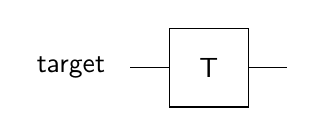
\begin{tikzpicture}[scale=.5] \node[draw=none] at (-3.5, 0) {target}; \draw (-2,0) -- (-1, 0); \draw (1, 0) -- (2, 0); \draw (-1,-1)--(-1,1)--(1,1)--(1,-1)--cycle; \node[draw=none] at (0, 0) {T}; \end{tikzpicture} } \]


\begin{DoxyParams}[1]{Parameters}
\mbox{\tt in,out}  & {\em multi\+Qubit} & object representing the set of all qubits \\
\hline
\mbox{\tt in}  & {\em target\+Qubit} & qubit to operate upon \\
\hline
\end{DoxyParams}

\begin{DoxyExceptions}{Exceptions}
{\em exit\+With\+Error} & if {\ttfamily target\+Qubit} is outside \mbox{[}0, {\ttfamily multi\+Qubit.\+num\+Qubits}) \\
\hline
\end{DoxyExceptions}


Definition at line 163 of file Qu\+E\+S\+T.\+cpp.



References phase\+Gate(), and T\+\_\+\+G\+A\+TE.


\begin{DoxyCode}
164 \{
165     \mbox{\hyperlink{QuEST__internal_8h_aae7a8a7f1ccbddb7f76b6c52b746bb43}{phaseGate}}(multiQubit, targetQubit, \mbox{\hyperlink{QuEST_8h_a5739021c733cecc49647956b2f7338eaa614d07d597a8e320cc556bc0e652e4ab}{T\_GATE}});
166 \}
\end{DoxyCode}
\mbox{\Hypertarget{QuEST_8cpp_ae2b2c14a07dd7d50ff86032a3ca101d7}\label{QuEST_8cpp_ae2b2c14a07dd7d50ff86032a3ca101d7}} 
\index{Qu\+E\+S\+T.\+cpp@{Qu\+E\+S\+T.\+cpp}!validate\+Alpha\+Beta@{validate\+Alpha\+Beta}}
\index{validate\+Alpha\+Beta@{validate\+Alpha\+Beta}!Qu\+E\+S\+T.\+cpp@{Qu\+E\+S\+T.\+cpp}}
\paragraph{\texorpdfstring{validate\+Alpha\+Beta()}{validateAlphaBeta()}}
{\footnotesize\ttfamily int validate\+Alpha\+Beta (\begin{DoxyParamCaption}\item[{\mbox{\hyperlink{structComplex}{Complex}}}]{alpha,  }\item[{\mbox{\hyperlink{structComplex}{Complex}}}]{beta }\end{DoxyParamCaption})}



Definition at line 193 of file Qu\+E\+S\+T.\+cpp.



References Complex\+::imag, Complex\+::real, and R\+E\+A\+L\+\_\+\+E\+PS.


\begin{DoxyCode}
193                                                   \{
194     \textcolor{keywordflow}{if} ( fabs(alpha.\mbox{\hyperlink{structComplex_a479ad939835457595fcca3ca55c06283}{real}}*alpha.\mbox{\hyperlink{structComplex_a479ad939835457595fcca3ca55c06283}{real}} 
195         + alpha.\mbox{\hyperlink{structComplex_a1151948284b21c0052f203f23ab931d9}{imag}}*alpha.\mbox{\hyperlink{structComplex_a1151948284b21c0052f203f23ab931d9}{imag}}
196         + beta.\mbox{\hyperlink{structComplex_a479ad939835457595fcca3ca55c06283}{real}}*beta.\mbox{\hyperlink{structComplex_a479ad939835457595fcca3ca55c06283}{real}} 
197         + beta.\mbox{\hyperlink{structComplex_a1151948284b21c0052f203f23ab931d9}{imag}}*beta.\mbox{\hyperlink{structComplex_a1151948284b21c0052f203f23ab931d9}{imag}} - 1) > \mbox{\hyperlink{QuEST__precision_8h_aebb5e6716e06431296af4d1a71744dec}{REAL\_EPS}} ) \textcolor{keywordflow}{return} 0;
198     \textcolor{keywordflow}{else} \textcolor{keywordflow}{return} 1;
199 \}
\end{DoxyCode}
\mbox{\Hypertarget{QuEST_8cpp_ae4fea133d1a8f09ff8da03038100adb2}\label{QuEST_8cpp_ae4fea133d1a8f09ff8da03038100adb2}} 
\index{Qu\+E\+S\+T.\+cpp@{Qu\+E\+S\+T.\+cpp}!validate\+Matrix\+Is\+Unitary@{validate\+Matrix\+Is\+Unitary}}
\index{validate\+Matrix\+Is\+Unitary@{validate\+Matrix\+Is\+Unitary}!Qu\+E\+S\+T.\+cpp@{Qu\+E\+S\+T.\+cpp}}
\paragraph{\texorpdfstring{validate\+Matrix\+Is\+Unitary()}{validateMatrixIsUnitary()}}
{\footnotesize\ttfamily int validate\+Matrix\+Is\+Unitary (\begin{DoxyParamCaption}\item[{\mbox{\hyperlink{structComplexMatrix2}{Complex\+Matrix2}}}]{u }\end{DoxyParamCaption})}



Definition at line 168 of file Qu\+E\+S\+T.\+cpp.



References Complex\+::imag, Complex\+Matrix2\+::r0c0, Complex\+Matrix2\+::r0c1, Complex\+Matrix2\+::r1c0, Complex\+Matrix2\+::r1c1, Complex\+::real, and R\+E\+A\+L\+\_\+\+E\+PS.


\begin{DoxyCode}
168                                              \{
169 
170     \textcolor{keywordflow}{if} ( fabs(u.\mbox{\hyperlink{structComplexMatrix2_ae72b4458233b077a636beee1892e81ff}{r0c0}}.\mbox{\hyperlink{structComplex_a479ad939835457595fcca3ca55c06283}{real}}*u.\mbox{\hyperlink{structComplexMatrix2_ae72b4458233b077a636beee1892e81ff}{r0c0}}.\mbox{\hyperlink{structComplex_a479ad939835457595fcca3ca55c06283}{real}} 
171         + u.\mbox{\hyperlink{structComplexMatrix2_ae72b4458233b077a636beee1892e81ff}{r0c0}}.\mbox{\hyperlink{structComplex_a1151948284b21c0052f203f23ab931d9}{imag}}*u.\mbox{\hyperlink{structComplexMatrix2_ae72b4458233b077a636beee1892e81ff}{r0c0}}.\mbox{\hyperlink{structComplex_a1151948284b21c0052f203f23ab931d9}{imag}}
172         + u.\mbox{\hyperlink{structComplexMatrix2_ab98282015ed2065e53fbc9638e2583ab}{r1c0}}.\mbox{\hyperlink{structComplex_a479ad939835457595fcca3ca55c06283}{real}}*u.\mbox{\hyperlink{structComplexMatrix2_ab98282015ed2065e53fbc9638e2583ab}{r1c0}}.\mbox{\hyperlink{structComplex_a479ad939835457595fcca3ca55c06283}{real}}
173         + u.\mbox{\hyperlink{structComplexMatrix2_ab98282015ed2065e53fbc9638e2583ab}{r1c0}}.\mbox{\hyperlink{structComplex_a1151948284b21c0052f203f23ab931d9}{imag}}*u.\mbox{\hyperlink{structComplexMatrix2_ab98282015ed2065e53fbc9638e2583ab}{r1c0}}.\mbox{\hyperlink{structComplex_a1151948284b21c0052f203f23ab931d9}{imag}} - 1) > \mbox{\hyperlink{QuEST__precision_8h_aebb5e6716e06431296af4d1a71744dec}{REAL\_EPS}} ) \textcolor{keywordflow}{return} 0;
174     \textcolor{comment}{// check}
175     \textcolor{keywordflow}{if} ( fabs(u.\mbox{\hyperlink{structComplexMatrix2_a0f3932f055a8b05cef361bce25d51172}{r0c1}}.\mbox{\hyperlink{structComplex_a479ad939835457595fcca3ca55c06283}{real}}*u.\mbox{\hyperlink{structComplexMatrix2_a0f3932f055a8b05cef361bce25d51172}{r0c1}}.\mbox{\hyperlink{structComplex_a479ad939835457595fcca3ca55c06283}{real}} 
176         + u.\mbox{\hyperlink{structComplexMatrix2_a0f3932f055a8b05cef361bce25d51172}{r0c1}}.\mbox{\hyperlink{structComplex_a1151948284b21c0052f203f23ab931d9}{imag}}*u.\mbox{\hyperlink{structComplexMatrix2_a0f3932f055a8b05cef361bce25d51172}{r0c1}}.\mbox{\hyperlink{structComplex_a1151948284b21c0052f203f23ab931d9}{imag}}
177         + u.\mbox{\hyperlink{structComplexMatrix2_a763007c3070802373549ba0350f83c8a}{r1c1}}.\mbox{\hyperlink{structComplex_a479ad939835457595fcca3ca55c06283}{real}}*u.\mbox{\hyperlink{structComplexMatrix2_a763007c3070802373549ba0350f83c8a}{r1c1}}.\mbox{\hyperlink{structComplex_a479ad939835457595fcca3ca55c06283}{real}}
178         + u.\mbox{\hyperlink{structComplexMatrix2_a763007c3070802373549ba0350f83c8a}{r1c1}}.\mbox{\hyperlink{structComplex_a1151948284b21c0052f203f23ab931d9}{imag}}*u.\mbox{\hyperlink{structComplexMatrix2_a763007c3070802373549ba0350f83c8a}{r1c1}}.\mbox{\hyperlink{structComplex_a1151948284b21c0052f203f23ab931d9}{imag}} - 1) > \mbox{\hyperlink{QuEST__precision_8h_aebb5e6716e06431296af4d1a71744dec}{REAL\_EPS}} ) \textcolor{keywordflow}{return} 0;
179 
180     \textcolor{keywordflow}{if} ( fabs(u.\mbox{\hyperlink{structComplexMatrix2_ae72b4458233b077a636beee1892e81ff}{r0c0}}.\mbox{\hyperlink{structComplex_a479ad939835457595fcca3ca55c06283}{real}}*u.\mbox{\hyperlink{structComplexMatrix2_a0f3932f055a8b05cef361bce25d51172}{r0c1}}.\mbox{\hyperlink{structComplex_a479ad939835457595fcca3ca55c06283}{real}} 
181         + u.\mbox{\hyperlink{structComplexMatrix2_ae72b4458233b077a636beee1892e81ff}{r0c0}}.\mbox{\hyperlink{structComplex_a1151948284b21c0052f203f23ab931d9}{imag}}*u.\mbox{\hyperlink{structComplexMatrix2_a0f3932f055a8b05cef361bce25d51172}{r0c1}}.\mbox{\hyperlink{structComplex_a1151948284b21c0052f203f23ab931d9}{imag}}
182         + u.\mbox{\hyperlink{structComplexMatrix2_ab98282015ed2065e53fbc9638e2583ab}{r1c0}}.\mbox{\hyperlink{structComplex_a479ad939835457595fcca3ca55c06283}{real}}*u.\mbox{\hyperlink{structComplexMatrix2_a763007c3070802373549ba0350f83c8a}{r1c1}}.\mbox{\hyperlink{structComplex_a479ad939835457595fcca3ca55c06283}{real}}
183         + u.\mbox{\hyperlink{structComplexMatrix2_ab98282015ed2065e53fbc9638e2583ab}{r1c0}}.\mbox{\hyperlink{structComplex_a1151948284b21c0052f203f23ab931d9}{imag}}*u.\mbox{\hyperlink{structComplexMatrix2_a763007c3070802373549ba0350f83c8a}{r1c1}}.\mbox{\hyperlink{structComplex_a1151948284b21c0052f203f23ab931d9}{imag}}) > \mbox{\hyperlink{QuEST__precision_8h_aebb5e6716e06431296af4d1a71744dec}{REAL\_EPS}} ) \textcolor{keywordflow}{return} 0;
184 
185     \textcolor{keywordflow}{if} ( fabs(u.\mbox{\hyperlink{structComplexMatrix2_a0f3932f055a8b05cef361bce25d51172}{r0c1}}.\mbox{\hyperlink{structComplex_a479ad939835457595fcca3ca55c06283}{real}}*u.\mbox{\hyperlink{structComplexMatrix2_ae72b4458233b077a636beee1892e81ff}{r0c0}}.\mbox{\hyperlink{structComplex_a1151948284b21c0052f203f23ab931d9}{imag}}
186         - u.\mbox{\hyperlink{structComplexMatrix2_ae72b4458233b077a636beee1892e81ff}{r0c0}}.\mbox{\hyperlink{structComplex_a479ad939835457595fcca3ca55c06283}{real}}*u.\mbox{\hyperlink{structComplexMatrix2_a0f3932f055a8b05cef361bce25d51172}{r0c1}}.\mbox{\hyperlink{structComplex_a1151948284b21c0052f203f23ab931d9}{imag}}
187         + u.\mbox{\hyperlink{structComplexMatrix2_a763007c3070802373549ba0350f83c8a}{r1c1}}.\mbox{\hyperlink{structComplex_a479ad939835457595fcca3ca55c06283}{real}}*u.\mbox{\hyperlink{structComplexMatrix2_ab98282015ed2065e53fbc9638e2583ab}{r1c0}}.\mbox{\hyperlink{structComplex_a1151948284b21c0052f203f23ab931d9}{imag}}
188         - u.\mbox{\hyperlink{structComplexMatrix2_ab98282015ed2065e53fbc9638e2583ab}{r1c0}}.\mbox{\hyperlink{structComplex_a479ad939835457595fcca3ca55c06283}{real}}*u.\mbox{\hyperlink{structComplexMatrix2_a763007c3070802373549ba0350f83c8a}{r1c1}}.\mbox{\hyperlink{structComplex_a1151948284b21c0052f203f23ab931d9}{imag}}) > \mbox{\hyperlink{QuEST__precision_8h_aebb5e6716e06431296af4d1a71744dec}{REAL\_EPS}} ) \textcolor{keywordflow}{return} 0;
189 
190     \textcolor{keywordflow}{return} 1;
191 \}
\end{DoxyCode}
\mbox{\Hypertarget{QuEST_8cpp_a71c14976f63cfcda70026fa20ee531fe}\label{QuEST_8cpp_a71c14976f63cfcda70026fa20ee531fe}} 
\index{Qu\+E\+S\+T.\+cpp@{Qu\+E\+S\+T.\+cpp}!validate\+Unit\+Vector@{validate\+Unit\+Vector}}
\index{validate\+Unit\+Vector@{validate\+Unit\+Vector}!Qu\+E\+S\+T.\+cpp@{Qu\+E\+S\+T.\+cpp}}
\paragraph{\texorpdfstring{validate\+Unit\+Vector()}{validateUnitVector()}}
{\footnotesize\ttfamily int validate\+Unit\+Vector (\begin{DoxyParamCaption}\item[{\mbox{\hyperlink{QuEST__precision_8h_a4b654506f18b8bfd61ad2a29a7e38c25}{R\+E\+AL}}}]{ux,  }\item[{\mbox{\hyperlink{QuEST__precision_8h_a4b654506f18b8bfd61ad2a29a7e38c25}{R\+E\+AL}}}]{uy,  }\item[{\mbox{\hyperlink{QuEST__precision_8h_a4b654506f18b8bfd61ad2a29a7e38c25}{R\+E\+AL}}}]{uz }\end{DoxyParamCaption})}



Definition at line 201 of file Qu\+E\+S\+T.\+cpp.



References R\+E\+A\+L\+\_\+\+E\+PS.


\begin{DoxyCode}
201                                                  \{
202     \textcolor{keywordflow}{if} ( fabs(sqrt(ux*ux + uy*uy + uz*uz) - 1) > \mbox{\hyperlink{QuEST__precision_8h_aebb5e6716e06431296af4d1a71744dec}{REAL\_EPS}} ) \textcolor{keywordflow}{return} 0;
203     \textcolor{keywordflow}{else} \textcolor{keywordflow}{return} 1;
204 \}
\end{DoxyCode}


\subsubsection{Variable Documentation}
\mbox{\Hypertarget{QuEST_8cpp_aac1637696885c75b73a1ecf381cea713}\label{QuEST_8cpp_aac1637696885c75b73a1ecf381cea713}} 
\index{Qu\+E\+S\+T.\+cpp@{Qu\+E\+S\+T.\+cpp}!error\+Codes@{error\+Codes}}
\index{error\+Codes@{error\+Codes}!Qu\+E\+S\+T.\+cpp@{Qu\+E\+S\+T.\+cpp}}
\paragraph{\texorpdfstring{error\+Codes}{errorCodes}}
{\footnotesize\ttfamily const char$\ast$ error\+Codes\mbox{[}$\,$\mbox{]}}

{\bfseries Initial value\+:}
\begin{DoxyCode}
= \{
    \textcolor{stringliteral}{"Success"},                                              
    \textcolor{stringliteral}{"Invalid target qubit. Note qubits are zero indexed."},  
    \textcolor{stringliteral}{"Invalid control qubit. Note qubits are zero indexed."}, 
    \textcolor{stringliteral}{"Control qubit cannot equal target qubit."},             
    \textcolor{stringliteral}{"Invalid number of control qubits"},                     
    \textcolor{stringliteral}{"Invalid unitary matrix."},                              
    \textcolor{stringliteral}{"Invalid rotation arguments."},                          
    \textcolor{stringliteral}{"Invalid system size. Cannot print output for systems greater than 5 qubits."}, 
    \textcolor{stringliteral}{"Can't collapse to state with zero probability."}, 
    \textcolor{stringliteral}{"Invalid number of qubits."}, 
    \textcolor{stringliteral}{"Invalid measurement outcome -- must be either 0 or 1."} 
\}
\end{DoxyCode}


Definition at line 24 of file Qu\+E\+S\+T.\+cpp.


\hypertarget{QuEST_8h}{}\subsection{Qu\+E\+S\+T.\+h File Reference}
\label{QuEST_8h}\index{Qu\+E\+S\+T.\+h@{Qu\+E\+S\+T.\+h}}


The Qu\+E\+ST library A\+PI and objects.  


{\ttfamily \#include \char`\"{}Qu\+E\+S\+T\+\_\+precision.\+h\char`\"{}}\newline
\subsubsection*{Data Structures}
\begin{DoxyCompactItemize}
\item 
struct \mbox{\hyperlink{structComplexArray}{Complex\+Array}}
\begin{DoxyCompactList}\small\item\em Represents an array of complex numbers grouped into an array of real components and an array of coressponding complex components. \end{DoxyCompactList}\item 
struct \mbox{\hyperlink{structComplex}{Complex}}
\begin{DoxyCompactList}\small\item\em Represents one complex number. \end{DoxyCompactList}\item 
struct \mbox{\hyperlink{structComplexMatrix2}{Complex\+Matrix2}}
\begin{DoxyCompactList}\small\item\em Represents a 2x2 matrix of complex numbers. \end{DoxyCompactList}\item 
struct \mbox{\hyperlink{structVector}{Vector}}
\item 
struct \mbox{\hyperlink{structMultiQubit}{Multi\+Qubit}}
\begin{DoxyCompactList}\small\item\em Represents a system of qubits. \end{DoxyCompactList}\item 
struct \mbox{\hyperlink{structQuESTEnv}{Qu\+E\+S\+T\+Env}}
\begin{DoxyCompactList}\small\item\em Information about the environment the program is running in. \end{DoxyCompactList}\end{DoxyCompactItemize}
\subsubsection*{Typedefs}
\begin{DoxyCompactItemize}
\item 
typedef struct \mbox{\hyperlink{structComplexArray}{Complex\+Array}} \mbox{\hyperlink{QuEST_8h_a19e00739fde70a851d068f322cf915c8}{Complex\+Array}}
\begin{DoxyCompactList}\small\item\em Represents an array of complex numbers grouped into an array of real components and an array of coressponding complex components. \end{DoxyCompactList}\item 
typedef struct \mbox{\hyperlink{structComplex}{Complex}} \mbox{\hyperlink{QuEST_8h_ad59c9e471673c07782e6c403277ffd8d}{Complex}}
\begin{DoxyCompactList}\small\item\em Represents one complex number. \end{DoxyCompactList}\item 
typedef struct \mbox{\hyperlink{structComplexMatrix2}{Complex\+Matrix2}} \mbox{\hyperlink{QuEST_8h_aa6e00518bd2c71030c52d5955e506875}{Complex\+Matrix2}}
\begin{DoxyCompactList}\small\item\em Represents a 2x2 matrix of complex numbers. \end{DoxyCompactList}\item 
typedef struct \mbox{\hyperlink{structVector}{Vector}} \mbox{\hyperlink{QuEST_8h_a6ded2cf071c127e518317e3c451af3ef}{Vector}}
\item 
typedef struct \mbox{\hyperlink{structMultiQubit}{Multi\+Qubit}} \mbox{\hyperlink{QuEST_8h_af4123a681074068eeeee1562758eef61}{Multi\+Qubit}}
\begin{DoxyCompactList}\small\item\em Represents a system of qubits. \end{DoxyCompactList}\item 
typedef struct \mbox{\hyperlink{structQuESTEnv}{Qu\+E\+S\+T\+Env}} \mbox{\hyperlink{QuEST_8h_aedfe2bb713c31d6133e53b1bd72d7a2c}{Qu\+E\+S\+T\+Env}}
\begin{DoxyCompactList}\small\item\em Information about the environment the program is running in. \end{DoxyCompactList}\end{DoxyCompactItemize}
\subsubsection*{Enumerations}
\begin{DoxyCompactItemize}
\item 
enum \mbox{\hyperlink{QuEST_8h_a5739021c733cecc49647956b2f7338ea}{phase\+Gate\+Type}} \{ \mbox{\hyperlink{QuEST_8h_a5739021c733cecc49647956b2f7338eaa754922d1e1846a1961ff2bf163483dac}{S\+I\+G\+M\+A\+\_\+Z}} =0, 
\mbox{\hyperlink{QuEST_8h_a5739021c733cecc49647956b2f7338eaa06e60f80fa80cce271793d6d31bcc21f}{S\+\_\+\+G\+A\+TE}} =1, 
\mbox{\hyperlink{QuEST_8h_a5739021c733cecc49647956b2f7338eaa614d07d597a8e320cc556bc0e652e4ab}{T\+\_\+\+G\+A\+TE}} =2
 \}
\end{DoxyCompactItemize}
\subsubsection*{Functions}
\begin{DoxyCompactItemize}
\item 
void \mbox{\hyperlink{QuEST_8h_a96f4de9ce7fefc7680a44d601fc3d894}{report\+State}} (\mbox{\hyperlink{structMultiQubit}{Multi\+Qubit}} multi\+Qubit)
\begin{DoxyCompactList}\small\item\em Print the current state vector of probability amplitudes for a set of qubits to file. \end{DoxyCompactList}\item 
void \mbox{\hyperlink{QuEST_8h_aa5e77e0e64f3a4a3d3f5cc7382bffcd9}{report\+Multi\+Qubit\+Params}} (\mbox{\hyperlink{structMultiQubit}{Multi\+Qubit}} multi\+Qubit)
\begin{DoxyCompactList}\small\item\em Report metainformation about a set of qubits\+: number of qubits, number of probability amplitudes. \end{DoxyCompactList}\item 
void \mbox{\hyperlink{QuEST_8h_a7fadb225fc385db789e844c87fcba9e1}{rotate\+Around\+Axis}} (\mbox{\hyperlink{structMultiQubit}{Multi\+Qubit}} multi\+Qubit, const int rot\+Qubit, \mbox{\hyperlink{QuEST__precision_8h_a4b654506f18b8bfd61ad2a29a7e38c25}{R\+E\+AL}} angle, \mbox{\hyperlink{structVector}{Vector}} unit\+Axis)
\begin{DoxyCompactList}\small\item\em Rotate a single qubit by a given angle around a given vector on the Bloch-\/sphere. \end{DoxyCompactList}\item 
void \mbox{\hyperlink{QuEST_8h_a6cc7fa705a2f2e6b486b49c5589d5df5}{rotateX}} (\mbox{\hyperlink{structMultiQubit}{Multi\+Qubit}} multi\+Qubit, const int rot\+Qubit, \mbox{\hyperlink{QuEST__precision_8h_a4b654506f18b8bfd61ad2a29a7e38c25}{R\+E\+AL}} angle)
\begin{DoxyCompactList}\small\item\em Rotate a single qubit by a given angle around the X-\/axis of the Bloch-\/sphere. \end{DoxyCompactList}\item 
void \mbox{\hyperlink{QuEST_8h_ace0d3592d38a990e81a434c4e9681500}{rotateY}} (\mbox{\hyperlink{structMultiQubit}{Multi\+Qubit}} multi\+Qubit, const int rot\+Qubit, \mbox{\hyperlink{QuEST__precision_8h_a4b654506f18b8bfd61ad2a29a7e38c25}{R\+E\+AL}} angle)
\begin{DoxyCompactList}\small\item\em Rotate a single qubit by a given angle around the Y-\/axis of the Bloch-\/sphere. \end{DoxyCompactList}\item 
void \mbox{\hyperlink{QuEST_8h_abd621412ad30c1b034f4ce153c4afe10}{rotateZ}} (\mbox{\hyperlink{structMultiQubit}{Multi\+Qubit}} multi\+Qubit, const int rot\+Qubit, \mbox{\hyperlink{QuEST__precision_8h_a4b654506f18b8bfd61ad2a29a7e38c25}{R\+E\+AL}} angle)
\begin{DoxyCompactList}\small\item\em Rotate a single qubit by a given angle around the Z-\/axis of the Bloch-\/sphere (also known as a phase shift gate). \end{DoxyCompactList}\item 
void \mbox{\hyperlink{QuEST_8h_ac6923ac57e67d9a21096e06f6a9012f6}{controlled\+RotateX}} (\mbox{\hyperlink{structMultiQubit}{Multi\+Qubit}} multi\+Qubit, const int control\+Qubit, const int target\+Qubit, \mbox{\hyperlink{QuEST__precision_8h_a4b654506f18b8bfd61ad2a29a7e38c25}{R\+E\+AL}} angle)
\begin{DoxyCompactList}\small\item\em Applies a controlled rotation by a given angle around the X-\/axis of the Bloch-\/sphere. \end{DoxyCompactList}\item 
void \mbox{\hyperlink{QuEST_8h_a71e90a2f7292116338c062934f9d1202}{controlled\+RotateY}} (\mbox{\hyperlink{structMultiQubit}{Multi\+Qubit}} multi\+Qubit, const int control\+Qubit, const int target\+Qubit, \mbox{\hyperlink{QuEST__precision_8h_a4b654506f18b8bfd61ad2a29a7e38c25}{R\+E\+AL}} angle)
\begin{DoxyCompactList}\small\item\em Applies a controlled rotation by a given angle around the Y-\/axis of the Bloch-\/sphere. \end{DoxyCompactList}\item 
void \mbox{\hyperlink{QuEST_8h_a668e5d2634b02e98bc73675ccb11d61c}{controlled\+RotateZ}} (\mbox{\hyperlink{structMultiQubit}{Multi\+Qubit}} multi\+Qubit, const int control\+Qubit, const int target\+Qubit, \mbox{\hyperlink{QuEST__precision_8h_a4b654506f18b8bfd61ad2a29a7e38c25}{R\+E\+AL}} angle)
\begin{DoxyCompactList}\small\item\em Applies a controlled rotation by a given angle around the Z-\/axis of the Bloch-\/sphere. \end{DoxyCompactList}\item 
void \mbox{\hyperlink{QuEST_8h_ad41f82b41149393a642391b67b3a287e}{controlled\+Rotate\+Around\+Axis}} (\mbox{\hyperlink{structMultiQubit}{Multi\+Qubit}} multi\+Qubit, const int control\+Qubit, const int target\+Qubit, \mbox{\hyperlink{QuEST__precision_8h_a4b654506f18b8bfd61ad2a29a7e38c25}{R\+E\+AL}} angle, \mbox{\hyperlink{structVector}{Vector}} axis)
\begin{DoxyCompactList}\small\item\em Applies a controlled rotation by a given angle around a given vector on the Bloch-\/sphere. \end{DoxyCompactList}\item 
void \mbox{\hyperlink{QuEST_8h_adda6c47876a7676488ed0565a19eaa65}{s\+Gate}} (\mbox{\hyperlink{structMultiQubit}{Multi\+Qubit}} multi\+Qubit, const int target\+Qubit)
\begin{DoxyCompactList}\small\item\em Apply the single-\/qubit S gate. \end{DoxyCompactList}\item 
void \mbox{\hyperlink{QuEST_8h_af764ea63a2e870098f4e1ce08562942e}{t\+Gate}} (\mbox{\hyperlink{structMultiQubit}{Multi\+Qubit}} multi\+Qubit, const int target\+Qubit)
\begin{DoxyCompactList}\small\item\em Apply the single-\/qubit T gate. \end{DoxyCompactList}\item 
void \mbox{\hyperlink{QuEST_8h_a8f10aabf9f607f19093aee54630caa21}{get\+Environment\+String}} (\mbox{\hyperlink{structQuESTEnv}{Qu\+E\+S\+T\+Env}} env, \mbox{\hyperlink{structMultiQubit}{Multi\+Qubit}} multi\+Qubit, char str\mbox{[}200\mbox{]})
\item 
void \mbox{\hyperlink{QuEST_8h_a842d6884e063a5865a2232cba56b65ac}{report\+State\+To\+Screen}} (\mbox{\hyperlink{structMultiQubit}{Multi\+Qubit}} multi\+Qubit, \mbox{\hyperlink{structQuESTEnv}{Qu\+E\+S\+T\+Env}} env, int report\+Rank)
\begin{DoxyCompactList}\small\item\em Print the current state vector of probability amplitudes for a set of qubits to standard out. \end{DoxyCompactList}\item 
void \mbox{\hyperlink{QuEST_8h_a11a96159191cbf1b01a1080e7f045aac}{controlled\+Phase\+Gate}} (\mbox{\hyperlink{structMultiQubit}{Multi\+Qubit}} multi\+Qubit, const int id\+Qubit1, const int id\+Qubit2)
\begin{DoxyCompactList}\small\item\em Apply the (two-\/qubit) controlled phase gate, also known as the controlled sigmaZ gate. \end{DoxyCompactList}\item 
void \mbox{\hyperlink{QuEST_8h_afc1835c6b43b6e59ce7df7b13f274fc7}{multi\+Controlled\+Phase\+Gate}} (\mbox{\hyperlink{structMultiQubit}{Multi\+Qubit}} multi\+Qubit, int $\ast$control\+Qubits, int num\+Control\+Qubits)
\begin{DoxyCompactList}\small\item\em Apply the multiple-\/qubit controlled phase gate, also known as the multiple-\/qubit controlled sigmaZ gate. \end{DoxyCompactList}\item 
void \mbox{\hyperlink{QuEST_8h_a67576895bbc65463481a8ea24d9b1e22}{controlled\+Not}} (\mbox{\hyperlink{structMultiQubit}{Multi\+Qubit}} multi\+Qubit, const int control\+Qubit, const int target\+Qubit)
\begin{DoxyCompactList}\small\item\em Apply the controlled not (single control, single target) gate, also known as the c-\/X, c-\/sigma-\/X, c-\/\+Pauli-\/X and c-\/bit-\/flip gate. \end{DoxyCompactList}\item 
void \mbox{\hyperlink{QuEST_8h_a9c02591bc64c2918503afa231d90d83f}{create\+Multi\+Qubit}} (\mbox{\hyperlink{structMultiQubit}{Multi\+Qubit}} $\ast$multi\+Qubit, int num\+Qubits, \mbox{\hyperlink{structQuESTEnv}{Qu\+E\+S\+T\+Env}} env)
\begin{DoxyCompactList}\small\item\em Create a \mbox{\hyperlink{structMultiQubit}{Multi\+Qubit}} object representing a set of qubits. \end{DoxyCompactList}\item 
void \mbox{\hyperlink{QuEST_8h_ae5d6acc322314d7a3d8a2eccf00d3b19}{destroy\+Multi\+Qubit}} (\mbox{\hyperlink{structMultiQubit}{Multi\+Qubit}} multi\+Qubit, \mbox{\hyperlink{structQuESTEnv}{Qu\+E\+S\+T\+Env}} env)
\begin{DoxyCompactList}\small\item\em Deallocate a \mbox{\hyperlink{structMultiQubit}{Multi\+Qubit}} object representing a set of qubits. \end{DoxyCompactList}\item 
void \mbox{\hyperlink{QuEST_8h_acb5b2eff794339090004d29f02a70d9a}{init\+State\+Zero}} (\mbox{\hyperlink{structMultiQubit}{Multi\+Qubit}} $\ast$multi\+Qubit)
\begin{DoxyCompactList}\small\item\em Initialise a set of $ N $ qubits to the classical zero state $ {| 0 \rangle}^{\otimes N} $. \end{DoxyCompactList}\item 
void \mbox{\hyperlink{QuEST_8h_a43bcb279fc9717fbd06a19cdef48b9d8}{init\+State\+Plus}} (\mbox{\hyperlink{structMultiQubit}{Multi\+Qubit}} $\ast$multi\+Qubit)
\begin{DoxyCompactList}\small\item\em Initialise a set of $ N $ qubits to the plus state $ {| + \rangle}^{\otimes N} = \frac{1}{\sqrt{2^N}} (| 0 \rangle + | 1 \rangle)^{\otimes N} $. \end{DoxyCompactList}\item 
void \mbox{\hyperlink{QuEST_8h_aea34d45aaea9e64ad3f7786bfb412d0c}{init\+Classical\+State}} (\mbox{\hyperlink{structMultiQubit}{Multi\+Qubit}} $\ast$multi\+Qubit, long long int state\+Ind)
\begin{DoxyCompactList}\small\item\em Initialise a set of $ N $ qubits to the classical state with index {\ttfamily state\+Ind}. \end{DoxyCompactList}\item 
void \mbox{\hyperlink{QuEST_8h_ad84a3ce68d1ca02b4e3f741ea45b6054}{init\+Qu\+E\+S\+T\+Env}} (\mbox{\hyperlink{structQuESTEnv}{Qu\+E\+S\+T\+Env}} $\ast$env)
\begin{DoxyCompactList}\small\item\em Initialize Qu\+E\+ST environment. \end{DoxyCompactList}\item 
void \mbox{\hyperlink{QuEST_8h_abd4bc926cd3f9b65610bb228d0c59fe0}{close\+Qu\+E\+S\+T\+Env}} (\mbox{\hyperlink{structQuESTEnv}{Qu\+E\+S\+T\+Env}} env)
\begin{DoxyCompactList}\small\item\em Initialize the Qu\+E\+ST environment. \end{DoxyCompactList}\item 
void \mbox{\hyperlink{QuEST_8h_a8d31fe2d1ad4d01e2a1f5f6b8bc15b77}{sync\+Qu\+E\+S\+T\+Env}} (\mbox{\hyperlink{structQuESTEnv}{Qu\+E\+S\+T\+Env}} env)
\begin{DoxyCompactList}\small\item\em Guarantees that all code up to the given point has been executed on all nodes. \end{DoxyCompactList}\item 
int \mbox{\hyperlink{QuEST_8h_ac7e38d768a1bd79019f88cc1e6295092}{sync\+Qu\+E\+S\+T\+Success}} (int success\+Code)
\begin{DoxyCompactList}\small\item\em Performs a logical A\+ND on all success\+Codes held by all processes. \end{DoxyCompactList}\item 
void \mbox{\hyperlink{QuEST_8h_af8a14ae79c3fb2c0b5f6255cc37bebf9}{report\+Qu\+E\+S\+T\+Env}} (\mbox{\hyperlink{structQuESTEnv}{Qu\+E\+S\+T\+Env}} env)
\begin{DoxyCompactList}\small\item\em Report information about the Qu\+E\+ST environment. \end{DoxyCompactList}\item 
\mbox{\hyperlink{QuEST__precision_8h_a4b654506f18b8bfd61ad2a29a7e38c25}{R\+E\+AL}} \mbox{\hyperlink{QuEST_8h_a818a4c7cd7252d2b10b896b12fa431d3}{calc\+Total\+Probability}} (\mbox{\hyperlink{structMultiQubit}{Multi\+Qubit}} multi\+Qubit)
\begin{DoxyCompactList}\small\item\em Calculate the probability of being in any state by taking the norm of the entire state vector. \end{DoxyCompactList}\item 
void \mbox{\hyperlink{QuEST_8h_ad13ae1902276195d0df106116e032aff}{compact\+Unitary}} (\mbox{\hyperlink{structMultiQubit}{Multi\+Qubit}} multi\+Qubit, const int rot\+Qubit, \mbox{\hyperlink{structComplex}{Complex}} alpha, \mbox{\hyperlink{structComplex}{Complex}} beta)
\begin{DoxyCompactList}\small\item\em Apply a single-\/qubit unitary parameterised by two given complex scalars. \end{DoxyCompactList}\item 
void \mbox{\hyperlink{QuEST_8h_ab4812953bc457405b3aa05a4c2f64f4a}{controlled\+Compact\+Unitary}} (\mbox{\hyperlink{structMultiQubit}{Multi\+Qubit}} multi\+Qubit, const int control\+Qubit, const int target\+Qubit, \mbox{\hyperlink{structComplex}{Complex}} alpha, \mbox{\hyperlink{structComplex}{Complex}} beta)
\begin{DoxyCompactList}\small\item\em Apply a controlled unitary (single control, single target) parameterised by two given complex scalars. \end{DoxyCompactList}\item 
void \mbox{\hyperlink{QuEST_8h_a7a0877e33700f6bad48adb51b7b3fb67}{unitary}} (\mbox{\hyperlink{structMultiQubit}{Multi\+Qubit}} multi\+Qubit, const int target\+Qubit, \mbox{\hyperlink{structComplexMatrix2}{Complex\+Matrix2}} u)
\begin{DoxyCompactList}\small\item\em Apply a general single-\/qubit unitary (including a global phase factor). \end{DoxyCompactList}\item 
void \mbox{\hyperlink{QuEST_8h_a8a701526263392599aa21d0d0f05d9d8}{controlled\+Unitary}} (\mbox{\hyperlink{structMultiQubit}{Multi\+Qubit}} multi\+Qubit, const int control\+Qubit, const int target\+Qubit, \mbox{\hyperlink{structComplexMatrix2}{Complex\+Matrix2}} u)
\begin{DoxyCompactList}\small\item\em Apply a general controlled unitary (single control, single target), which can include a global phase factor. \end{DoxyCompactList}\item 
void \mbox{\hyperlink{QuEST_8h_ae395a79690283ed81106afadd7a8cd8a}{multi\+Controlled\+Unitary}} (\mbox{\hyperlink{structMultiQubit}{Multi\+Qubit}} multi\+Qubit, int $\ast$control\+Qubits, const int num\+Control\+Qubits, const int target\+Qubit, \mbox{\hyperlink{structComplexMatrix2}{Complex\+Matrix2}} u)
\begin{DoxyCompactList}\small\item\em Apply a general multiple-\/control single-\/target unitary, which can include a global phase factor. \end{DoxyCompactList}\item 
void \mbox{\hyperlink{QuEST_8h_a86e396e06b7d527cac20ba0108872423}{sigmaX}} (\mbox{\hyperlink{structMultiQubit}{Multi\+Qubit}} multi\+Qubit, const int target\+Qubit)
\begin{DoxyCompactList}\small\item\em Apply the single-\/qubit sigma-\/X (also known as the X, Pauli-\/X, N\+OT or bit-\/flip) gate. \end{DoxyCompactList}\item 
void \mbox{\hyperlink{QuEST_8h_a1f54d70a42403f7e1c2e2c2007332f61}{sigmaY}} (\mbox{\hyperlink{structMultiQubit}{Multi\+Qubit}} multi\+Qubit, const int target\+Qubit)
\begin{DoxyCompactList}\small\item\em Apply the single-\/qubit sigma-\/Y (also known as the Y or Pauli-\/Y) gate. \end{DoxyCompactList}\item 
void \mbox{\hyperlink{QuEST_8h_aebaab86326779de55d335cfea3efde8f}{sigmaZ}} (\mbox{\hyperlink{structMultiQubit}{Multi\+Qubit}} multi\+Qubit, const int target\+Qubit)
\begin{DoxyCompactList}\small\item\em Apply the single-\/qubit sigma-\/Z (also known as the Z, Pauli-\/Z or phase-\/flip) gate. \end{DoxyCompactList}\item 
void \mbox{\hyperlink{QuEST_8h_aa09b5dd93de6df1384b8f2c0041749ab}{hadamard}} (\mbox{\hyperlink{structMultiQubit}{Multi\+Qubit}} multi\+Qubit, const int target\+Qubit)
\begin{DoxyCompactList}\small\item\em Apply the single-\/qubit Hadamard gate. \end{DoxyCompactList}\item 
\mbox{\hyperlink{QuEST__precision_8h_a4b654506f18b8bfd61ad2a29a7e38c25}{R\+E\+AL}} \mbox{\hyperlink{QuEST_8h_ad315c941a51bc053d39ebfa2040fd32e}{find\+Probability\+Of\+Outcome}} (\mbox{\hyperlink{structMultiQubit}{Multi\+Qubit}} multi\+Qubit, const int measure\+Qubit, int outcome)
\begin{DoxyCompactList}\small\item\em Gives the probability of a specified qubit being measured in the given outcome (0 or 1). \end{DoxyCompactList}\item 
\mbox{\hyperlink{QuEST__precision_8h_a4b654506f18b8bfd61ad2a29a7e38c25}{R\+E\+AL}} \mbox{\hyperlink{QuEST_8h_a07418ebac70fd9ae5d051d089961631d}{collapse\+To\+Outcome}} (\mbox{\hyperlink{structMultiQubit}{Multi\+Qubit}} multi\+Qubit, const int measure\+Qubit, int outcome)
\begin{DoxyCompactList}\small\item\em Updates the state vector to be consistent with measuring the measure qubit in the given outcome (0 or 1), and returns the probability of such a measurement outcome. \end{DoxyCompactList}\item 
int \mbox{\hyperlink{QuEST_8h_ad5774247d836267175c664cd0e451bcb}{measure}} (\mbox{\hyperlink{structMultiQubit}{Multi\+Qubit}} multi\+Qubit, int measure\+Qubit)
\begin{DoxyCompactList}\small\item\em Measures a single qubit, collapsing it randomly to 0 or 1. \end{DoxyCompactList}\item 
int \mbox{\hyperlink{QuEST_8h_a2ac46e470c750bf93c754e06c64b0a7a}{measure\+With\+Stats}} (\mbox{\hyperlink{structMultiQubit}{Multi\+Qubit}} multi\+Qubit, int measure\+Qubit, \mbox{\hyperlink{QuEST__precision_8h_a4b654506f18b8bfd61ad2a29a7e38c25}{R\+E\+AL}} $\ast$state\+Prob)
\begin{DoxyCompactList}\small\item\em Measures a single qubit, collapsing it randomly to 0 or 1, and additionally gives the probability of that outcome. \end{DoxyCompactList}\item 
void \mbox{\hyperlink{QuEST_8h_ac49f548ee27ae484695f9add1273adb4}{Qu\+E\+S\+T\+Seed\+Random\+Default}} (void)
\begin{DoxyCompactList}\small\item\em Seed the Mersenne Twister used for random number generation in the Qu\+E\+ST environment with an example defualt seed. \end{DoxyCompactList}\item 
void \mbox{\hyperlink{QuEST_8h_aedb5ef39da69e7895d714980dc621261}{Qu\+E\+S\+T\+Seed\+Random}} (unsigned long int $\ast$seed\+Array, int num\+Seeds)
\begin{DoxyCompactList}\small\item\em Seed the Mersenne Twister used for random number generation in the Qu\+E\+ST environment with a user defined seed. \end{DoxyCompactList}\end{DoxyCompactItemize}


\subsubsection{Detailed Description}
The Qu\+E\+ST library A\+PI and objects. 



\subsubsection{Typedef Documentation}
\mbox{\Hypertarget{QuEST_8h_ad59c9e471673c07782e6c403277ffd8d}\label{QuEST_8h_ad59c9e471673c07782e6c403277ffd8d}} 
\index{Qu\+E\+S\+T.\+h@{Qu\+E\+S\+T.\+h}!Complex@{Complex}}
\index{Complex@{Complex}!Qu\+E\+S\+T.\+h@{Qu\+E\+S\+T.\+h}}
\paragraph{\texorpdfstring{Complex}{Complex}}
{\footnotesize\ttfamily typedef struct \mbox{\hyperlink{structComplex}{Complex}}  \mbox{\hyperlink{structComplex}{Complex}}}



Represents one complex number. 

\mbox{\Hypertarget{QuEST_8h_a19e00739fde70a851d068f322cf915c8}\label{QuEST_8h_a19e00739fde70a851d068f322cf915c8}} 
\index{Qu\+E\+S\+T.\+h@{Qu\+E\+S\+T.\+h}!Complex\+Array@{Complex\+Array}}
\index{Complex\+Array@{Complex\+Array}!Qu\+E\+S\+T.\+h@{Qu\+E\+S\+T.\+h}}
\paragraph{\texorpdfstring{Complex\+Array}{ComplexArray}}
{\footnotesize\ttfamily typedef struct \mbox{\hyperlink{structComplexArray}{Complex\+Array}}  \mbox{\hyperlink{structComplexArray}{Complex\+Array}}}



Represents an array of complex numbers grouped into an array of real components and an array of coressponding complex components. 

\mbox{\Hypertarget{QuEST_8h_aa6e00518bd2c71030c52d5955e506875}\label{QuEST_8h_aa6e00518bd2c71030c52d5955e506875}} 
\index{Qu\+E\+S\+T.\+h@{Qu\+E\+S\+T.\+h}!Complex\+Matrix2@{Complex\+Matrix2}}
\index{Complex\+Matrix2@{Complex\+Matrix2}!Qu\+E\+S\+T.\+h@{Qu\+E\+S\+T.\+h}}
\paragraph{\texorpdfstring{Complex\+Matrix2}{ComplexMatrix2}}
{\footnotesize\ttfamily typedef struct \mbox{\hyperlink{structComplexMatrix2}{Complex\+Matrix2}}  \mbox{\hyperlink{structComplexMatrix2}{Complex\+Matrix2}}}



Represents a 2x2 matrix of complex numbers. 

\mbox{\Hypertarget{QuEST_8h_af4123a681074068eeeee1562758eef61}\label{QuEST_8h_af4123a681074068eeeee1562758eef61}} 
\index{Qu\+E\+S\+T.\+h@{Qu\+E\+S\+T.\+h}!Multi\+Qubit@{Multi\+Qubit}}
\index{Multi\+Qubit@{Multi\+Qubit}!Qu\+E\+S\+T.\+h@{Qu\+E\+S\+T.\+h}}
\paragraph{\texorpdfstring{Multi\+Qubit}{MultiQubit}}
{\footnotesize\ttfamily typedef struct \mbox{\hyperlink{structMultiQubit}{Multi\+Qubit}}  \mbox{\hyperlink{structMultiQubit}{Multi\+Qubit}}}



Represents a system of qubits. 

Qubits are zero-\/based and the the first qubit is the rightmost \mbox{\Hypertarget{QuEST_8h_aedfe2bb713c31d6133e53b1bd72d7a2c}\label{QuEST_8h_aedfe2bb713c31d6133e53b1bd72d7a2c}} 
\index{Qu\+E\+S\+T.\+h@{Qu\+E\+S\+T.\+h}!Qu\+E\+S\+T\+Env@{Qu\+E\+S\+T\+Env}}
\index{Qu\+E\+S\+T\+Env@{Qu\+E\+S\+T\+Env}!Qu\+E\+S\+T.\+h@{Qu\+E\+S\+T.\+h}}
\paragraph{\texorpdfstring{Qu\+E\+S\+T\+Env}{QuESTEnv}}
{\footnotesize\ttfamily typedef struct \mbox{\hyperlink{structQuESTEnv}{Qu\+E\+S\+T\+Env}}  \mbox{\hyperlink{structQuESTEnv}{Qu\+E\+S\+T\+Env}}}



Information about the environment the program is running in. 

In practice, this holds info about M\+PI ranks and helps to hide M\+PI initialization code \mbox{\Hypertarget{QuEST_8h_a6ded2cf071c127e518317e3c451af3ef}\label{QuEST_8h_a6ded2cf071c127e518317e3c451af3ef}} 
\index{Qu\+E\+S\+T.\+h@{Qu\+E\+S\+T.\+h}!Vector@{Vector}}
\index{Vector@{Vector}!Qu\+E\+S\+T.\+h@{Qu\+E\+S\+T.\+h}}
\paragraph{\texorpdfstring{Vector}{Vector}}
{\footnotesize\ttfamily typedef struct \mbox{\hyperlink{structVector}{Vector}}  \mbox{\hyperlink{structVector}{Vector}}}



\subsubsection{Enumeration Type Documentation}
\mbox{\Hypertarget{QuEST_8h_a5739021c733cecc49647956b2f7338ea}\label{QuEST_8h_a5739021c733cecc49647956b2f7338ea}} 
\index{Qu\+E\+S\+T.\+h@{Qu\+E\+S\+T.\+h}!phase\+Gate\+Type@{phase\+Gate\+Type}}
\index{phase\+Gate\+Type@{phase\+Gate\+Type}!Qu\+E\+S\+T.\+h@{Qu\+E\+S\+T.\+h}}
\paragraph{\texorpdfstring{phase\+Gate\+Type}{phaseGateType}}
{\footnotesize\ttfamily enum \mbox{\hyperlink{QuEST_8h_a5739021c733cecc49647956b2f7338ea}{phase\+Gate\+Type}}}

\begin{DoxyEnumFields}{Enumerator}
\raisebox{\heightof{T}}[0pt][0pt]{\index{S\+I\+G\+M\+A\+\_\+Z@{S\+I\+G\+M\+A\+\_\+Z}!Qu\+E\+S\+T.\+h@{Qu\+E\+S\+T.\+h}}\index{Qu\+E\+S\+T.\+h@{Qu\+E\+S\+T.\+h}!S\+I\+G\+M\+A\+\_\+Z@{S\+I\+G\+M\+A\+\_\+Z}}}\mbox{\Hypertarget{QuEST_8h_a5739021c733cecc49647956b2f7338eaa754922d1e1846a1961ff2bf163483dac}\label{QuEST_8h_a5739021c733cecc49647956b2f7338eaa754922d1e1846a1961ff2bf163483dac}} 
S\+I\+G\+M\+A\+\_\+Z&\\
\hline

\raisebox{\heightof{T}}[0pt][0pt]{\index{S\+\_\+\+G\+A\+TE@{S\+\_\+\+G\+A\+TE}!Qu\+E\+S\+T.\+h@{Qu\+E\+S\+T.\+h}}\index{Qu\+E\+S\+T.\+h@{Qu\+E\+S\+T.\+h}!S\+\_\+\+G\+A\+TE@{S\+\_\+\+G\+A\+TE}}}\mbox{\Hypertarget{QuEST_8h_a5739021c733cecc49647956b2f7338eaa06e60f80fa80cce271793d6d31bcc21f}\label{QuEST_8h_a5739021c733cecc49647956b2f7338eaa06e60f80fa80cce271793d6d31bcc21f}} 
S\+\_\+\+G\+A\+TE&\\
\hline

\raisebox{\heightof{T}}[0pt][0pt]{\index{T\+\_\+\+G\+A\+TE@{T\+\_\+\+G\+A\+TE}!Qu\+E\+S\+T.\+h@{Qu\+E\+S\+T.\+h}}\index{Qu\+E\+S\+T.\+h@{Qu\+E\+S\+T.\+h}!T\+\_\+\+G\+A\+TE@{T\+\_\+\+G\+A\+TE}}}\mbox{\Hypertarget{QuEST_8h_a5739021c733cecc49647956b2f7338eaa614d07d597a8e320cc556bc0e652e4ab}\label{QuEST_8h_a5739021c733cecc49647956b2f7338eaa614d07d597a8e320cc556bc0e652e4ab}} 
T\+\_\+\+G\+A\+TE&\\
\hline

\end{DoxyEnumFields}


Definition at line 79 of file Qu\+E\+S\+T.\+h.


\begin{DoxyCode}
79 \{\mbox{\hyperlink{QuEST_8h_a5739021c733cecc49647956b2f7338eaa754922d1e1846a1961ff2bf163483dac}{SIGMA\_Z}}=0, \mbox{\hyperlink{QuEST_8h_a5739021c733cecc49647956b2f7338eaa06e60f80fa80cce271793d6d31bcc21f}{S\_GATE}}=1, \mbox{\hyperlink{QuEST_8h_a5739021c733cecc49647956b2f7338eaa614d07d597a8e320cc556bc0e652e4ab}{T\_GATE}}=2\};
\end{DoxyCode}


\subsubsection{Function Documentation}
\mbox{\Hypertarget{QuEST_8h_a818a4c7cd7252d2b10b896b12fa431d3}\label{QuEST_8h_a818a4c7cd7252d2b10b896b12fa431d3}} 
\index{Qu\+E\+S\+T.\+h@{Qu\+E\+S\+T.\+h}!calc\+Total\+Probability@{calc\+Total\+Probability}}
\index{calc\+Total\+Probability@{calc\+Total\+Probability}!Qu\+E\+S\+T.\+h@{Qu\+E\+S\+T.\+h}}
\paragraph{\texorpdfstring{calc\+Total\+Probability()}{calcTotalProbability()}}
{\footnotesize\ttfamily \mbox{\hyperlink{QuEST__precision_8h_a4b654506f18b8bfd61ad2a29a7e38c25}{R\+E\+AL}} calc\+Total\+Probability (\begin{DoxyParamCaption}\item[{\mbox{\hyperlink{structMultiQubit}{Multi\+Qubit}}}]{multi\+Qubit }\end{DoxyParamCaption})}



Calculate the probability of being in any state by taking the norm of the entire state vector. 

Should be equal to 1.


\begin{DoxyParams}[1]{Parameters}
\mbox{\tt in}  & {\em multi\+Qubit} & object representing a set of qubits \\
\hline
\end{DoxyParams}
\begin{DoxyReturn}{Returns}
total probability 
\end{DoxyReturn}
\mbox{\Hypertarget{QuEST_8h_abd4bc926cd3f9b65610bb228d0c59fe0}\label{QuEST_8h_abd4bc926cd3f9b65610bb228d0c59fe0}} 
\index{Qu\+E\+S\+T.\+h@{Qu\+E\+S\+T.\+h}!close\+Qu\+E\+S\+T\+Env@{close\+Qu\+E\+S\+T\+Env}}
\index{close\+Qu\+E\+S\+T\+Env@{close\+Qu\+E\+S\+T\+Env}!Qu\+E\+S\+T.\+h@{Qu\+E\+S\+T.\+h}}
\paragraph{\texorpdfstring{close\+Qu\+E\+S\+T\+Env()}{closeQuESTEnv()}}
{\footnotesize\ttfamily void close\+Qu\+E\+S\+T\+Env (\begin{DoxyParamCaption}\item[{\mbox{\hyperlink{structQuESTEnv}{Qu\+E\+S\+T\+Env}}}]{env }\end{DoxyParamCaption})}



Initialize the Qu\+E\+ST environment. 

If something needs to be done to set up the execution environment, such as initializing M\+PI when running in distributed mode, it is handled here


\begin{DoxyParams}[1]{Parameters}
\mbox{\tt in,out}  & {\em env} & object representing the execution environment. A single instance is used for each program \\
\hline
\end{DoxyParams}
\mbox{\Hypertarget{QuEST_8h_a07418ebac70fd9ae5d051d089961631d}\label{QuEST_8h_a07418ebac70fd9ae5d051d089961631d}} 
\index{Qu\+E\+S\+T.\+h@{Qu\+E\+S\+T.\+h}!collapse\+To\+Outcome@{collapse\+To\+Outcome}}
\index{collapse\+To\+Outcome@{collapse\+To\+Outcome}!Qu\+E\+S\+T.\+h@{Qu\+E\+S\+T.\+h}}
\paragraph{\texorpdfstring{collapse\+To\+Outcome()}{collapseToOutcome()}}
{\footnotesize\ttfamily \mbox{\hyperlink{QuEST__precision_8h_a4b654506f18b8bfd61ad2a29a7e38c25}{R\+E\+AL}} collapse\+To\+Outcome (\begin{DoxyParamCaption}\item[{\mbox{\hyperlink{structMultiQubit}{Multi\+Qubit}}}]{multi\+Qubit,  }\item[{const int}]{measure\+Qubit,  }\item[{int}]{outcome }\end{DoxyParamCaption})}



Updates the state vector to be consistent with measuring the measure qubit in the given outcome (0 or 1), and returns the probability of such a measurement outcome. 

This is effectively performing a measurement and forcing the outcome. This is an irreversible change to the state vector, whereby incompatible states in the state vector are given zero amplitude and the remaining states are renormalised. Exits with error if the given outcome has $\sim$zero probability, and so cannot be collapsed into.


\begin{DoxyParams}[1]{Parameters}
\mbox{\tt in,out}  & {\em multi\+Qubit} & object representing the set of all qubits \\
\hline
\mbox{\tt in}  & {\em measure\+Qubit} & qubit to measure \\
\hline
\mbox{\tt in}  & {\em outcome} & to force the measure qubit to enter \\
\hline
\end{DoxyParams}
\begin{DoxyReturn}{Returns}
probability of the (forced) measurement outcome 
\end{DoxyReturn}

\begin{DoxyExceptions}{Exceptions}
{\em exit\+With\+Error} & if {\ttfamily measure\+Qubit} is outside \mbox{[}0, {\ttfamily multi\+Qubit.\+num\+Qubits}), or if {\ttfamily outcome} is not in \{0, 1\}, or if the probability of {\ttfamily outcome} is zero (within machine epsilon) \\
\hline
\end{DoxyExceptions}
\mbox{\Hypertarget{QuEST_8h_ad13ae1902276195d0df106116e032aff}\label{QuEST_8h_ad13ae1902276195d0df106116e032aff}} 
\index{Qu\+E\+S\+T.\+h@{Qu\+E\+S\+T.\+h}!compact\+Unitary@{compact\+Unitary}}
\index{compact\+Unitary@{compact\+Unitary}!Qu\+E\+S\+T.\+h@{Qu\+E\+S\+T.\+h}}
\paragraph{\texorpdfstring{compact\+Unitary()}{compactUnitary()}}
{\footnotesize\ttfamily void compact\+Unitary (\begin{DoxyParamCaption}\item[{\mbox{\hyperlink{structMultiQubit}{Multi\+Qubit}}}]{multi\+Qubit,  }\item[{const int}]{rot\+Qubit,  }\item[{\mbox{\hyperlink{structComplex}{Complex}}}]{alpha,  }\item[{\mbox{\hyperlink{structComplex}{Complex}}}]{beta }\end{DoxyParamCaption})}



Apply a single-\/qubit unitary parameterised by two given complex scalars. 

Given valid complex numbers $\alpha$ and $\beta$, applies the unitary \[ U = \begin{pmatrix} \alpha & -\beta^* \\ \beta & \alpha^* \end{pmatrix} \] which is general up to a global phase factor. ~\newline
Valid $\alpha$, $\beta$ satisfy $|\alpha|^2 + |\beta|^2 = 1$.

\[ \setlength{\fboxrule}{0.01pt} \fbox{ 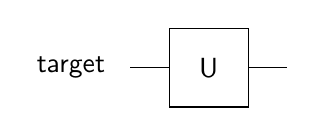
\begin{tikzpicture}[scale=.5] \node[draw=none] at (-3.5, 0) {target}; \draw (-2,0) -- (-1, 0); \draw (1, 0) -- (2, 0); \draw (-1,-1)--(-1,1)--(1,1)--(1,-1)--cycle; \node[draw=none] at (0, 0) {U}; \end{tikzpicture} } \]


\begin{DoxyParams}[1]{Parameters}
\mbox{\tt in,out}  & {\em multi\+Qubit} & object representing the set of all qubits \\
\hline
\mbox{\tt in}  & {\em target\+Qubit} & qubit to operate on \\
\hline
\mbox{\tt in}  & {\em alpha} & complex unitary parameter (row 1, column 1) \\
\hline
\mbox{\tt in}  & {\em beta} & complex unitary parameter (row 2, column 1) \\
\hline
\end{DoxyParams}

\begin{DoxyExceptions}{Exceptions}
{\em exit\+With\+Error} & if {\ttfamily target\+Qubit} is outside \mbox{[}0, {\ttfamily multi\+Qubit.\+num\+Qubits}), or if {\ttfamily alpha}, {\ttfamily beta} don\textquotesingle{}t satisfy $\vert${\ttfamily alpha$\vert$$^\wedge$2} + $\vert${\ttfamily beta$\vert$$^\wedge$2} = 1. \\
\hline
\end{DoxyExceptions}


Referenced by rotate\+Around\+Axis().

\mbox{\Hypertarget{QuEST_8h_ab4812953bc457405b3aa05a4c2f64f4a}\label{QuEST_8h_ab4812953bc457405b3aa05a4c2f64f4a}} 
\index{Qu\+E\+S\+T.\+h@{Qu\+E\+S\+T.\+h}!controlled\+Compact\+Unitary@{controlled\+Compact\+Unitary}}
\index{controlled\+Compact\+Unitary@{controlled\+Compact\+Unitary}!Qu\+E\+S\+T.\+h@{Qu\+E\+S\+T.\+h}}
\paragraph{\texorpdfstring{controlled\+Compact\+Unitary()}{controlledCompactUnitary()}}
{\footnotesize\ttfamily void controlled\+Compact\+Unitary (\begin{DoxyParamCaption}\item[{\mbox{\hyperlink{structMultiQubit}{Multi\+Qubit}}}]{multi\+Qubit,  }\item[{const int}]{control\+Qubit,  }\item[{const int}]{target\+Qubit,  }\item[{\mbox{\hyperlink{structComplex}{Complex}}}]{alpha,  }\item[{\mbox{\hyperlink{structComplex}{Complex}}}]{beta }\end{DoxyParamCaption})}



Apply a controlled unitary (single control, single target) parameterised by two given complex scalars. 

Given valid complex numbers $\alpha$ and $\beta$, applies the two-\/qubit unitary \[ \begin{pmatrix} 1 \\ & 1 \\ & & \alpha & -\beta^* \\ & & \beta & \alpha^* \end{pmatrix} \] to the control and target qubits. Valid $\alpha$, $\beta$ satisfy $|\alpha|^2 + |\beta|^2 = 1$. The target unitary is general up to a global phase factor. ~\newline
 \[ \setlength{\fboxrule}{0.01pt} \fbox{ 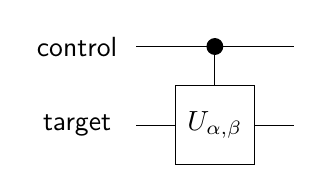
\begin{tikzpicture}[scale=.5] \node[draw=none] at (-3.5, 2) {control}; \node[draw=none] at (-3.5, 0) {target}; \draw (-2, 2) -- (2, 2); \draw[fill=black] (0, 2) circle (.2); \draw (0, 2) -- (0, 1); \draw (-2,0) -- (-1, 0); \draw (1, 0) -- (2, 0); \draw (-1,-1)--(-1,1)--(1,1)--(1,-1)--cycle; \node[draw=none] at (0, 0) {$U_{\alpha, \beta}$}; \end{tikzpicture} } \]


\begin{DoxyParams}[1]{Parameters}
\mbox{\tt in,out}  & {\em multi\+Qubit} & object representing the set of all qubits \\
\hline
\mbox{\tt in}  & {\em control\+Qubit} & apply the target unitary if this qubit has value 1 \\
\hline
\mbox{\tt in}  & {\em target\+Qubit} & qubit on which to apply the target unitary \\
\hline
\mbox{\tt in}  & {\em alpha} & complex unitary parameter (row 1, column 1) \\
\hline
\mbox{\tt in}  & {\em beta} & complex unitary parameter (row 2, column 1) \\
\hline
\end{DoxyParams}

\begin{DoxyExceptions}{Exceptions}
{\em exit\+With\+Error} & if either {\ttfamily control\+Qubit} or {\ttfamily target\+Qubit} are outside \mbox{[}0, {\ttfamily multi\+Qubit.\+num\+Qubits}) or are equal, or if {\ttfamily alpha}, {\ttfamily beta} don\textquotesingle{}t satisfy $\vert${\ttfamily alpha$\vert$$^\wedge$2} + $\vert${\ttfamily beta$\vert$$^\wedge$2} = 1. \\
\hline
\end{DoxyExceptions}


Referenced by controlled\+Rotate\+Around\+Axis().

\mbox{\Hypertarget{QuEST_8h_a67576895bbc65463481a8ea24d9b1e22}\label{QuEST_8h_a67576895bbc65463481a8ea24d9b1e22}} 
\index{Qu\+E\+S\+T.\+h@{Qu\+E\+S\+T.\+h}!controlled\+Not@{controlled\+Not}}
\index{controlled\+Not@{controlled\+Not}!Qu\+E\+S\+T.\+h@{Qu\+E\+S\+T.\+h}}
\paragraph{\texorpdfstring{controlled\+Not()}{controlledNot()}}
{\footnotesize\ttfamily void controlled\+Not (\begin{DoxyParamCaption}\item[{\mbox{\hyperlink{structMultiQubit}{Multi\+Qubit}}}]{multi\+Qubit,  }\item[{const int}]{control\+Qubit,  }\item[{const int}]{target\+Qubit }\end{DoxyParamCaption})}



Apply the controlled not (single control, single target) gate, also known as the c-\/X, c-\/sigma-\/X, c-\/\+Pauli-\/X and c-\/bit-\/flip gate. 

This applies sigmaX to the target qubit if the control qubit has value 1. This effects the two-\/qubit unitary \[ \begin{pmatrix} 1 \\ & 1 \\\ & & & 1 \\ & & 1 \end{pmatrix} \] on the control and target qubits.

\[ \setlength{\fboxrule}{0.01pt} \fbox{ 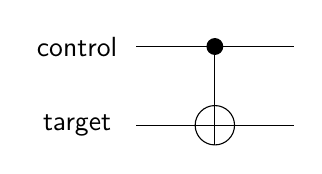
\begin{tikzpicture}[scale=.5] \node[draw=none] at (-3.5, 2) {control}; \node[draw=none] at (-3.5, 0) {target}; \draw (-2, 2) -- (2, 2); \draw[fill=black] (0, 2) circle (.2); \draw (0, 2) -- (0, -.5); \draw (-2,0) -- (2, 0); \draw (0, 0) circle (.5); \end{tikzpicture} } \] ~\newline
 
\begin{DoxyParams}[1]{Parameters}
\mbox{\tt in,out}  & {\em multi\+Qubit} & object representing the set of all qubits \\
\hline
\mbox{\tt in}  & {\em control\+Qubit} & nots the target if this qubit is 1 \\
\hline
\mbox{\tt in}  & {\em target\+Qubit} & qubit to not \\
\hline
\end{DoxyParams}

\begin{DoxyExceptions}{Exceptions}
{\em exit\+With\+Error} & if either {\ttfamily control\+Qubit} or {\ttfamily target\+Qubit} are outside \mbox{[}0, {\ttfamily multi\+Qubit.\+num\+Qubits}), or are equal. \\
\hline
\end{DoxyExceptions}
\mbox{\Hypertarget{QuEST_8h_a11a96159191cbf1b01a1080e7f045aac}\label{QuEST_8h_a11a96159191cbf1b01a1080e7f045aac}} 
\index{Qu\+E\+S\+T.\+h@{Qu\+E\+S\+T.\+h}!controlled\+Phase\+Gate@{controlled\+Phase\+Gate}}
\index{controlled\+Phase\+Gate@{controlled\+Phase\+Gate}!Qu\+E\+S\+T.\+h@{Qu\+E\+S\+T.\+h}}
\paragraph{\texorpdfstring{controlled\+Phase\+Gate()}{controlledPhaseGate()}}
{\footnotesize\ttfamily void controlled\+Phase\+Gate (\begin{DoxyParamCaption}\item[{\mbox{\hyperlink{structMultiQubit}{Multi\+Qubit}}}]{multi\+Qubit,  }\item[{const int}]{id\+Qubit1,  }\item[{const int}]{id\+Qubit2 }\end{DoxyParamCaption})}



Apply the (two-\/qubit) controlled phase gate, also known as the controlled sigmaZ gate. 

For each state, if both input qubits have value one, multiply the amplitude of that state by -\/1. This applies the two-\/qubit unitary\+: \[ \begin{pmatrix} 1 \\ & 1 \\\ & & 1 \\ & & & -1 \end{pmatrix} \]

\[ \setlength{\fboxrule}{0.01pt} \fbox{ 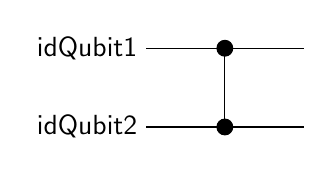
\begin{tikzpicture}[scale=.5] \node[draw=none] at (-3.5, 2) {idQubit1}; \node[draw=none] at (-3.5, 0) {idQubit2}; \draw (-2, 2) -- (2, 2); \draw[fill=black] (0, 2) circle (.2); \draw (0, 2) -- (0, 0); \draw (-2,0) -- (2, 0); \draw[fill=black] (0, 0) circle (.2); \end{tikzpicture} } \]


\begin{DoxyParams}[1]{Parameters}
\mbox{\tt in,out}  & {\em multi\+Qubit} & object representing the set of all qubits \\
\hline
\mbox{\tt in}  & {\em id\+Qubit1,id\+Qubit2} & qubits to operate upon \\
\hline
\end{DoxyParams}

\begin{DoxyExceptions}{Exceptions}
{\em exit\+With\+Error} & if {\ttfamily id\+Qubit1} or {\ttfamily id\+Qubit2} are outside \mbox{[}0, {\ttfamily multi\+Qubit.\+num\+Qubits}), or are equal \\
\hline
\end{DoxyExceptions}
\mbox{\Hypertarget{QuEST_8h_ad41f82b41149393a642391b67b3a287e}\label{QuEST_8h_ad41f82b41149393a642391b67b3a287e}} 
\index{Qu\+E\+S\+T.\+h@{Qu\+E\+S\+T.\+h}!controlled\+Rotate\+Around\+Axis@{controlled\+Rotate\+Around\+Axis}}
\index{controlled\+Rotate\+Around\+Axis@{controlled\+Rotate\+Around\+Axis}!Qu\+E\+S\+T.\+h@{Qu\+E\+S\+T.\+h}}
\paragraph{\texorpdfstring{controlled\+Rotate\+Around\+Axis()}{controlledRotateAroundAxis()}}
{\footnotesize\ttfamily void controlled\+Rotate\+Around\+Axis (\begin{DoxyParamCaption}\item[{\mbox{\hyperlink{structMultiQubit}{Multi\+Qubit}}}]{multi\+Qubit,  }\item[{const int}]{control\+Qubit,  }\item[{const int}]{target\+Qubit,  }\item[{\mbox{\hyperlink{QuEST__precision_8h_a4b654506f18b8bfd61ad2a29a7e38c25}{R\+E\+AL}}}]{angle,  }\item[{\mbox{\hyperlink{structVector}{Vector}}}]{axis }\end{DoxyParamCaption})}



Applies a controlled rotation by a given angle around a given vector on the Bloch-\/sphere. 

The vector must not be zero (else an error is thrown), but needn\textquotesingle{}t be unit magnitude.

For angle $\theta$ and axis vector $\vec{n}$, applies $R_{\hat{n}} = \exp \left(- i \frac{\theta}{2} \hat{n} \cdot \vec{\sigma} \right) $ to states where the target qubit is 1 ( $\vec{\sigma}$ is the vector of Pauli matrices).

\[ \setlength{\fboxrule}{0.01pt} \fbox{ 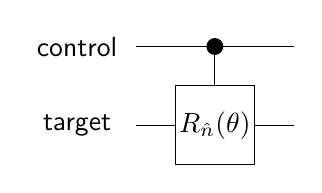
\begin{tikzpicture}[scale=.5] \node[draw=none] at (-3.5, 2) {control}; \node[draw=none] at (-3.5, 0) {target}; \draw (-2, 2) -- (2, 2); \draw[fill=black] (0, 2) circle (.2); \draw (0, 2) -- (0, 1); \draw (-2,0) -- (-1, 0); \draw (1, 0) -- (2, 0); \draw (-1,-1)--(-1,1)--(1,1)--(1,-1)--cycle; \node[draw=none] at (0, 0) {$R_{\hat{n}}(\theta)$}; \end{tikzpicture} } \]


\begin{DoxyParams}[1]{Parameters}
\mbox{\tt in,out}  & {\em multi\+Qubit} & object representing the set of all qubits \\
\hline
\mbox{\tt in}  & {\em control\+Qubit} & qubit with value 1 in the rotated states \\
\hline
\mbox{\tt in}  & {\em target\+Qubit} & qubit to rotate \\
\hline
\mbox{\tt in}  & {\em angle} & angle by which to rotate in radians \\
\hline
\mbox{\tt in}  & {\em axis} & vector around which to rotate (can be non-\/unit; will be normalised) \\
\hline
\end{DoxyParams}

\begin{DoxyExceptions}{Exceptions}
{\em exit\+With\+Error} & if either {\ttfamily control\+Qubit} or {\ttfamily target\+Qubit} are outside \mbox{[}0, {\ttfamily multi\+Qubit.\+num\+Qubits}) or are equal or if {\ttfamily axis} is the zero vector \\
\hline
\end{DoxyExceptions}


Definition at line 122 of file Qu\+E\+S\+T.\+cpp.



References controlled\+Compact\+Unitary(), Complex\+::imag, Complex\+::real, Vector\+::x, Vector\+::y, and Vector\+::z.



Referenced by controlled\+Rotate\+X(), controlled\+Rotate\+Y(), and controlled\+Rotate\+Z().


\begin{DoxyCode}
122                                                                                                            
                         \{
123 
124     \textcolor{keywordtype}{double} mag = sqrt(pow(axis.\mbox{\hyperlink{structVector_aac7abe171ba4bada50ed72acba6259fc}{x}},2) + pow(axis.\mbox{\hyperlink{structVector_a375ca805d4c808a53d7c4e0c737ae3de}{y}},2) + pow(axis.\mbox{\hyperlink{structVector_ad4e863651be7d6b7e2b28cd7445a0ccf}{z}},2));
125     \mbox{\hyperlink{structVector}{Vector}} unitAxis = \{axis.\mbox{\hyperlink{structVector_aac7abe171ba4bada50ed72acba6259fc}{x}}/mag, axis.\mbox{\hyperlink{structVector_a375ca805d4c808a53d7c4e0c737ae3de}{y}}/mag, axis.\mbox{\hyperlink{structVector_ad4e863651be7d6b7e2b28cd7445a0ccf}{z}}/mag\};
126 
127     \mbox{\hyperlink{structComplex}{Complex}} alpha, beta;
128     alpha.\mbox{\hyperlink{structComplex_a479ad939835457595fcca3ca55c06283}{real}} = cos(angle/2.0);
129     alpha.\mbox{\hyperlink{structComplex_a1151948284b21c0052f203f23ab931d9}{imag}} = -sin(angle/2.0)*unitAxis.\mbox{\hyperlink{structVector_ad4e863651be7d6b7e2b28cd7445a0ccf}{z}};    
130     beta.\mbox{\hyperlink{structComplex_a479ad939835457595fcca3ca55c06283}{real}} = sin(angle/2.0)*unitAxis.\mbox{\hyperlink{structVector_a375ca805d4c808a53d7c4e0c737ae3de}{y}};
131     beta.\mbox{\hyperlink{structComplex_a1151948284b21c0052f203f23ab931d9}{imag}} = -sin(angle/2.0)*unitAxis.\mbox{\hyperlink{structVector_aac7abe171ba4bada50ed72acba6259fc}{x}};
132     \mbox{\hyperlink{QuEST_8h_ab4812953bc457405b3aa05a4c2f64f4a}{controlledCompactUnitary}}(multiQubit, controlQubit, targetQubit, alpha, beta);
133 \}
\end{DoxyCode}
\mbox{\Hypertarget{QuEST_8h_ac6923ac57e67d9a21096e06f6a9012f6}\label{QuEST_8h_ac6923ac57e67d9a21096e06f6a9012f6}} 
\index{Qu\+E\+S\+T.\+h@{Qu\+E\+S\+T.\+h}!controlled\+RotateX@{controlled\+RotateX}}
\index{controlled\+RotateX@{controlled\+RotateX}!Qu\+E\+S\+T.\+h@{Qu\+E\+S\+T.\+h}}
\paragraph{\texorpdfstring{controlled\+Rotate\+X()}{controlledRotateX()}}
{\footnotesize\ttfamily void controlled\+RotateX (\begin{DoxyParamCaption}\item[{\mbox{\hyperlink{structMultiQubit}{Multi\+Qubit}}}]{multi\+Qubit,  }\item[{const int}]{control\+Qubit,  }\item[{const int}]{target\+Qubit,  }\item[{\mbox{\hyperlink{QuEST__precision_8h_a4b654506f18b8bfd61ad2a29a7e38c25}{R\+E\+AL}}}]{angle }\end{DoxyParamCaption})}



Applies a controlled rotation by a given angle around the X-\/axis of the Bloch-\/sphere. 

The target qubit is rotated in states where the control qubit has value 1.

\[ \setlength{\fboxrule}{0.01pt} \fbox{ 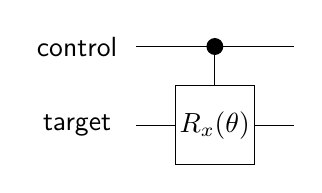
\begin{tikzpicture}[scale=.5] \node[draw=none] at (-3.5, 2) {control}; \node[draw=none] at (-3.5, 0) {target}; \draw (-2, 2) -- (2, 2); \draw[fill=black] (0, 2) circle (.2); \draw (0, 2) -- (0, 1); \draw (-2,0) -- (-1, 0); \draw (1, 0) -- (2, 0); \draw (-1,-1)--(-1,1)--(1,1)--(1,-1)--cycle; \node[draw=none] at (0, 0) {$R_x(\theta)$}; \end{tikzpicture} } \] ~\newline
 
\begin{DoxyParams}[1]{Parameters}
\mbox{\tt in,out}  & {\em multi\+Qubit} & object representing the set of all qubits \\
\hline
\mbox{\tt in}  & {\em control\+Qubit} & qubit which has value 1 in the rotated states \\
\hline
\mbox{\tt in}  & {\em tagret\+Qubit} & qubit to rotate \\
\hline
\mbox{\tt in}  & {\em angle} & angle by which to rotate the target qubit in radians \\
\hline
\end{DoxyParams}

\begin{DoxyExceptions}{Exceptions}
{\em exit\+With\+Error} & if either {\ttfamily control\+Qubit} or {\ttfamily target\+Qubit} are outside \mbox{[}0, {\ttfamily multi\+Qubit.\+num\+Qubits}) or are equal. \\
\hline
\end{DoxyExceptions}


Definition at line 135 of file Qu\+E\+S\+T.\+cpp.



References controlled\+Rotate\+Around\+Axis().


\begin{DoxyCode}
135                                                                                                         \{
136 
137     \mbox{\hyperlink{structVector}{Vector}} unitAxis = \{1, 0, 0\};
138     \mbox{\hyperlink{QuEST_8cpp_ad41f82b41149393a642391b67b3a287e}{controlledRotateAroundAxis}}(multiQubit, controlQubit, targetQubit, angle, 
      unitAxis);
139 \}
\end{DoxyCode}
\mbox{\Hypertarget{QuEST_8h_a71e90a2f7292116338c062934f9d1202}\label{QuEST_8h_a71e90a2f7292116338c062934f9d1202}} 
\index{Qu\+E\+S\+T.\+h@{Qu\+E\+S\+T.\+h}!controlled\+RotateY@{controlled\+RotateY}}
\index{controlled\+RotateY@{controlled\+RotateY}!Qu\+E\+S\+T.\+h@{Qu\+E\+S\+T.\+h}}
\paragraph{\texorpdfstring{controlled\+Rotate\+Y()}{controlledRotateY()}}
{\footnotesize\ttfamily void controlled\+RotateY (\begin{DoxyParamCaption}\item[{\mbox{\hyperlink{structMultiQubit}{Multi\+Qubit}}}]{multi\+Qubit,  }\item[{const int}]{control\+Qubit,  }\item[{const int}]{target\+Qubit,  }\item[{\mbox{\hyperlink{QuEST__precision_8h_a4b654506f18b8bfd61ad2a29a7e38c25}{R\+E\+AL}}}]{angle }\end{DoxyParamCaption})}



Applies a controlled rotation by a given angle around the Y-\/axis of the Bloch-\/sphere. 

The target qubit is rotated in states where the control qubit has value 1.

\[ \setlength{\fboxrule}{0.01pt} \fbox{ 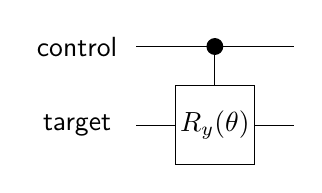
\begin{tikzpicture}[scale=.5] \node[draw=none] at (-3.5, 2) {control}; \node[draw=none] at (-3.5, 0) {target}; \draw (-2, 2) -- (2, 2); \draw[fill=black] (0, 2) circle (.2); \draw (0, 2) -- (0, 1); \draw (-2,0) -- (-1, 0); \draw (1, 0) -- (2, 0); \draw (-1,-1)--(-1,1)--(1,1)--(1,-1)--cycle; \node[draw=none] at (0, 0) {$R_y(\theta)$}; \end{tikzpicture} } \] ~\newline
 
\begin{DoxyParams}[1]{Parameters}
\mbox{\tt in,out}  & {\em multi\+Qubit} & object representing the set of all qubits \\
\hline
\mbox{\tt in}  & {\em control\+Qubit} & qubit which has value 1 in the rotated states \\
\hline
\mbox{\tt in}  & {\em tagret\+Qubit} & qubit to rotate \\
\hline
\mbox{\tt in}  & {\em angle} & angle by which to rotate the target qubit in radians \\
\hline
\end{DoxyParams}

\begin{DoxyExceptions}{Exceptions}
{\em exit\+With\+Error} & if either {\ttfamily control\+Qubit} or {\ttfamily target\+Qubit} are outside \mbox{[}0, {\ttfamily multi\+Qubit.\+num\+Qubits}) or are equal. \\
\hline
\end{DoxyExceptions}


Definition at line 141 of file Qu\+E\+S\+T.\+cpp.



References controlled\+Rotate\+Around\+Axis().


\begin{DoxyCode}
141                                                                                                         \{
142 
143     \mbox{\hyperlink{structVector}{Vector}} unitAxis = \{0, 1, 0\};
144     \mbox{\hyperlink{QuEST_8cpp_ad41f82b41149393a642391b67b3a287e}{controlledRotateAroundAxis}}(multiQubit, controlQubit, targetQubit, angle, 
      unitAxis);
145 \}
\end{DoxyCode}
\mbox{\Hypertarget{QuEST_8h_a668e5d2634b02e98bc73675ccb11d61c}\label{QuEST_8h_a668e5d2634b02e98bc73675ccb11d61c}} 
\index{Qu\+E\+S\+T.\+h@{Qu\+E\+S\+T.\+h}!controlled\+RotateZ@{controlled\+RotateZ}}
\index{controlled\+RotateZ@{controlled\+RotateZ}!Qu\+E\+S\+T.\+h@{Qu\+E\+S\+T.\+h}}
\paragraph{\texorpdfstring{controlled\+Rotate\+Z()}{controlledRotateZ()}}
{\footnotesize\ttfamily void controlled\+RotateZ (\begin{DoxyParamCaption}\item[{\mbox{\hyperlink{structMultiQubit}{Multi\+Qubit}}}]{multi\+Qubit,  }\item[{const int}]{control\+Qubit,  }\item[{const int}]{target\+Qubit,  }\item[{\mbox{\hyperlink{QuEST__precision_8h_a4b654506f18b8bfd61ad2a29a7e38c25}{R\+E\+AL}}}]{angle }\end{DoxyParamCaption})}



Applies a controlled rotation by a given angle around the Z-\/axis of the Bloch-\/sphere. 

The target qubit is rotated in states where the control qubit has value 1.

\[ \setlength{\fboxrule}{0.01pt} \fbox{ 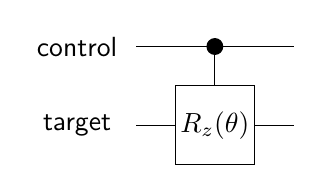
\begin{tikzpicture}[scale=.5] \node[draw=none] at (-3.5, 2) {control}; \node[draw=none] at (-3.5, 0) {target}; \draw (-2, 2) -- (2, 2); \draw[fill=black] (0, 2) circle (.2); \draw (0, 2) -- (0, 1); \draw (-2,0) -- (-1, 0); \draw (1, 0) -- (2, 0); \draw (-1,-1)--(-1,1)--(1,1)--(1,-1)--cycle; \node[draw=none] at (0, 0) {$R_z(\theta)$}; \end{tikzpicture} } \] ~\newline
 
\begin{DoxyParams}[1]{Parameters}
\mbox{\tt in,out}  & {\em multi\+Qubit} & object representing the set of all qubits \\
\hline
\mbox{\tt in}  & {\em control\+Qubit} & qubit which has value 1 in the rotated states \\
\hline
\mbox{\tt in}  & {\em tagret\+Qubit} & qubit to rotate \\
\hline
\mbox{\tt in}  & {\em angle} & angle by which to rotate the target qubit in radians \\
\hline
\end{DoxyParams}

\begin{DoxyExceptions}{Exceptions}
{\em exit\+With\+Error} & if either {\ttfamily control\+Qubit} or {\ttfamily target\+Qubit} are outside \mbox{[}0, {\ttfamily multi\+Qubit.\+num\+Qubits}) or are equal. \\
\hline
\end{DoxyExceptions}


Definition at line 147 of file Qu\+E\+S\+T.\+cpp.



References controlled\+Rotate\+Around\+Axis().


\begin{DoxyCode}
147                                                                                                         \{
148 
149     \mbox{\hyperlink{structVector}{Vector}} unitAxis = \{0, 0, 1\};
150     \mbox{\hyperlink{QuEST_8cpp_ad41f82b41149393a642391b67b3a287e}{controlledRotateAroundAxis}}(multiQubit, controlQubit, targetQubit, angle, 
      unitAxis);
151 \}
\end{DoxyCode}
\mbox{\Hypertarget{QuEST_8h_a8a701526263392599aa21d0d0f05d9d8}\label{QuEST_8h_a8a701526263392599aa21d0d0f05d9d8}} 
\index{Qu\+E\+S\+T.\+h@{Qu\+E\+S\+T.\+h}!controlled\+Unitary@{controlled\+Unitary}}
\index{controlled\+Unitary@{controlled\+Unitary}!Qu\+E\+S\+T.\+h@{Qu\+E\+S\+T.\+h}}
\paragraph{\texorpdfstring{controlled\+Unitary()}{controlledUnitary()}}
{\footnotesize\ttfamily void controlled\+Unitary (\begin{DoxyParamCaption}\item[{\mbox{\hyperlink{structMultiQubit}{Multi\+Qubit}}}]{multi\+Qubit,  }\item[{const int}]{control\+Qubit,  }\item[{const int}]{target\+Qubit,  }\item[{\mbox{\hyperlink{structComplexMatrix2}{Complex\+Matrix2}}}]{u }\end{DoxyParamCaption})}



Apply a general controlled unitary (single control, single target), which can include a global phase factor. 

The given unitary is applied to the target qubit if the control qubit has value 1, effecting the two-\/qubit unitary \[ \begin{pmatrix} 1 \\ & 1 \\ & & u_{00} & u_{01}\\ & & u_{10} & u_{11} \end{pmatrix} \] on the control and target qubits.

\[ \setlength{\fboxrule}{0.01pt} \fbox{ 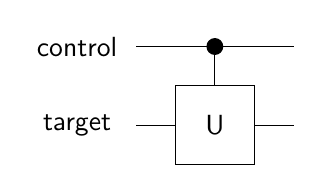
\begin{tikzpicture}[scale=.5] \node[draw=none] at (-3.5, 2) {control}; \node[draw=none] at (-3.5, 0) {target}; \draw (-2, 2) -- (2, 2); \draw[fill=black] (0, 2) circle (.2); \draw (0, 2) -- (0, 1); \draw (-2,0) -- (-1, 0); \draw (1, 0) -- (2, 0); \draw (-1,-1)--(-1,1)--(1,1)--(1,-1)--cycle; \node[draw=none] at (0, 0) {U}; \end{tikzpicture} } \]


\begin{DoxyParams}[1]{Parameters}
\mbox{\tt in,out}  & {\em multi\+Qubit} & object representing the set of all qubits \\
\hline
\mbox{\tt in}  & {\em control\+Qubit} & apply unitary if this qubit is 1 \\
\hline
\mbox{\tt in}  & {\em target\+Qubit} & qubit to operate on \\
\hline
\mbox{\tt in}  & {\em u} & single-\/qubit unitary matrix to apply \\
\hline
\end{DoxyParams}

\begin{DoxyExceptions}{Exceptions}
{\em exit\+With\+Error} & if either {\ttfamily control\+Qubit} or {\ttfamily target\+Qubit} are outside \mbox{[}0, {\ttfamily multi\+Qubit.\+num\+Qubits}) or are equal, or if {\ttfamily u} is not unitary. \\
\hline
\end{DoxyExceptions}
\mbox{\Hypertarget{QuEST_8h_a9c02591bc64c2918503afa231d90d83f}\label{QuEST_8h_a9c02591bc64c2918503afa231d90d83f}} 
\index{Qu\+E\+S\+T.\+h@{Qu\+E\+S\+T.\+h}!create\+Multi\+Qubit@{create\+Multi\+Qubit}}
\index{create\+Multi\+Qubit@{create\+Multi\+Qubit}!Qu\+E\+S\+T.\+h@{Qu\+E\+S\+T.\+h}}
\paragraph{\texorpdfstring{create\+Multi\+Qubit()}{createMultiQubit()}}
{\footnotesize\ttfamily void create\+Multi\+Qubit (\begin{DoxyParamCaption}\item[{\mbox{\hyperlink{structMultiQubit}{Multi\+Qubit}} $\ast$}]{multi\+Qubit,  }\item[{int}]{num\+Qubits,  }\item[{\mbox{\hyperlink{structQuESTEnv}{Qu\+E\+S\+T\+Env}}}]{env }\end{DoxyParamCaption})}



Create a \mbox{\hyperlink{structMultiQubit}{Multi\+Qubit}} object representing a set of qubits. 

Allocate space for state vector of probability amplitudes, including space for temporary values to be copied from one other chunk if running the distributed version. Define properties related to the size of the set of qubits. init\+State\+Zero should be called after this to initialise the qubits to the zero state.


\begin{DoxyParams}[1]{Parameters}
\mbox{\tt in,out}  & {\em multi\+Qubit} & a pointer to an object representing the set of qubits \\
\hline
\mbox{\tt in}  & {\em num\+Qubits} & number of qubits in the system \\
\hline
\mbox{\tt in}  & {\em env} & object representing the execution environment (local, multinode etc) \\
\hline
\end{DoxyParams}

\begin{DoxyExceptions}{Exceptions}
{\em exit\+With\+Error} & if {\ttfamily num\+Qubits} $<$= 0 \\
\hline
\end{DoxyExceptions}
\mbox{\Hypertarget{QuEST_8h_ae5d6acc322314d7a3d8a2eccf00d3b19}\label{QuEST_8h_ae5d6acc322314d7a3d8a2eccf00d3b19}} 
\index{Qu\+E\+S\+T.\+h@{Qu\+E\+S\+T.\+h}!destroy\+Multi\+Qubit@{destroy\+Multi\+Qubit}}
\index{destroy\+Multi\+Qubit@{destroy\+Multi\+Qubit}!Qu\+E\+S\+T.\+h@{Qu\+E\+S\+T.\+h}}
\paragraph{\texorpdfstring{destroy\+Multi\+Qubit()}{destroyMultiQubit()}}
{\footnotesize\ttfamily void destroy\+Multi\+Qubit (\begin{DoxyParamCaption}\item[{\mbox{\hyperlink{structMultiQubit}{Multi\+Qubit}}}]{multi\+Qubit,  }\item[{\mbox{\hyperlink{structQuESTEnv}{Qu\+E\+S\+T\+Env}}}]{env }\end{DoxyParamCaption})}



Deallocate a \mbox{\hyperlink{structMultiQubit}{Multi\+Qubit}} object representing a set of qubits. 

Free memory allocated to state vector of probability amplitudes, including temporary vector for values copied from another chunk if running the distributed version.


\begin{DoxyParams}[1]{Parameters}
\mbox{\tt in,out}  & {\em multi\+Qubit} & object to be deallocated \\
\hline
\mbox{\tt in}  & {\em env} & object representing the execution environment (local, multinode etc) \\
\hline
\end{DoxyParams}
\mbox{\Hypertarget{QuEST_8h_ad315c941a51bc053d39ebfa2040fd32e}\label{QuEST_8h_ad315c941a51bc053d39ebfa2040fd32e}} 
\index{Qu\+E\+S\+T.\+h@{Qu\+E\+S\+T.\+h}!find\+Probability\+Of\+Outcome@{find\+Probability\+Of\+Outcome}}
\index{find\+Probability\+Of\+Outcome@{find\+Probability\+Of\+Outcome}!Qu\+E\+S\+T.\+h@{Qu\+E\+S\+T.\+h}}
\paragraph{\texorpdfstring{find\+Probability\+Of\+Outcome()}{findProbabilityOfOutcome()}}
{\footnotesize\ttfamily \mbox{\hyperlink{QuEST__precision_8h_a4b654506f18b8bfd61ad2a29a7e38c25}{R\+E\+AL}} find\+Probability\+Of\+Outcome (\begin{DoxyParamCaption}\item[{\mbox{\hyperlink{structMultiQubit}{Multi\+Qubit}}}]{multi\+Qubit,  }\item[{const int}]{measure\+Qubit,  }\item[{int}]{outcome }\end{DoxyParamCaption})}



Gives the probability of a specified qubit being measured in the given outcome (0 or 1). 

This performs no actual measurement and does not change the state of the qubits.


\begin{DoxyParams}[1]{Parameters}
\mbox{\tt in}  & {\em multi\+Qubit} & object representing the set of all qubits \\
\hline
\mbox{\tt in}  & {\em measure\+Qubit} & qubit to study \\
\hline
\mbox{\tt in}  & {\em outcome} & for which to find the probability of the qubit being measured in \\
\hline
\end{DoxyParams}
\begin{DoxyReturn}{Returns}
probability of qubit measure\+Qubit being measured in the given outcome 
\end{DoxyReturn}

\begin{DoxyExceptions}{Exceptions}
{\em exit\+With\+Error} & if {\ttfamily measure\+Qubit} is outside \mbox{[}0, {\ttfamily multi\+Qubit.\+num\+Qubits}), or if {\ttfamily outcome} is not in \{0, 1\}. \\
\hline
\end{DoxyExceptions}
\mbox{\Hypertarget{QuEST_8h_a8f10aabf9f607f19093aee54630caa21}\label{QuEST_8h_a8f10aabf9f607f19093aee54630caa21}} 
\index{Qu\+E\+S\+T.\+h@{Qu\+E\+S\+T.\+h}!get\+Environment\+String@{get\+Environment\+String}}
\index{get\+Environment\+String@{get\+Environment\+String}!Qu\+E\+S\+T.\+h@{Qu\+E\+S\+T.\+h}}
\paragraph{\texorpdfstring{get\+Environment\+String()}{getEnvironmentString()}}
{\footnotesize\ttfamily void get\+Environment\+String (\begin{DoxyParamCaption}\item[{\mbox{\hyperlink{structQuESTEnv}{Qu\+E\+S\+T\+Env}}}]{env,  }\item[{\mbox{\hyperlink{structMultiQubit}{Multi\+Qubit}}}]{multi\+Qubit,  }\item[{char}]{str\mbox{[}200\mbox{]} }\end{DoxyParamCaption})}

\mbox{\Hypertarget{QuEST_8h_aa09b5dd93de6df1384b8f2c0041749ab}\label{QuEST_8h_aa09b5dd93de6df1384b8f2c0041749ab}} 
\index{Qu\+E\+S\+T.\+h@{Qu\+E\+S\+T.\+h}!hadamard@{hadamard}}
\index{hadamard@{hadamard}!Qu\+E\+S\+T.\+h@{Qu\+E\+S\+T.\+h}}
\paragraph{\texorpdfstring{hadamard()}{hadamard()}}
{\footnotesize\ttfamily void hadamard (\begin{DoxyParamCaption}\item[{\mbox{\hyperlink{structMultiQubit}{Multi\+Qubit}}}]{multi\+Qubit,  }\item[{const int}]{target\+Qubit }\end{DoxyParamCaption})}



Apply the single-\/qubit Hadamard gate. 

This takes $|0\rangle$ to $|+\rangle$ and $|1\rangle$ to $|-\rangle$, and is equivalent to a rotation of $\pi$ around the x-\/axis then $\pi/2$ about the y-\/axis on the Bloch-\/sphere. I.\+e. \[ \frac{1}{\sqrt{2}} \begin{pmatrix} 1 & 1 \\ 1 & -1 \end{pmatrix} \] ~\newline
 \[ \setlength{\fboxrule}{0.01pt} \fbox{ 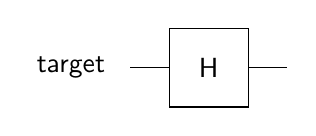
\begin{tikzpicture}[scale=.5] \node[draw=none] at (-3.5, 0) {target}; \draw (-2,0) -- (-1, 0); \draw (1, 0) -- (2, 0); \draw (-1,-1)--(-1,1)--(1,1)--(1,-1)--cycle; \node[draw=none] at (0, 0) {H}; \end{tikzpicture} } \] ~\newline
 
\begin{DoxyParams}[1]{Parameters}
\mbox{\tt in,out}  & {\em multi\+Qubit} & object representing the set of all qubits \\
\hline
\mbox{\tt in}  & {\em target\+Qubit} & qubit to operate on \\
\hline
\end{DoxyParams}

\begin{DoxyExceptions}{Exceptions}
{\em exit\+With\+Error} & if {\ttfamily target\+Qubit} is outside \mbox{[}0, {\ttfamily multi\+Qubit.\+num\+Qubits}). \\
\hline
\end{DoxyExceptions}
\mbox{\Hypertarget{QuEST_8h_aea34d45aaea9e64ad3f7786bfb412d0c}\label{QuEST_8h_aea34d45aaea9e64ad3f7786bfb412d0c}} 
\index{Qu\+E\+S\+T.\+h@{Qu\+E\+S\+T.\+h}!init\+Classical\+State@{init\+Classical\+State}}
\index{init\+Classical\+State@{init\+Classical\+State}!Qu\+E\+S\+T.\+h@{Qu\+E\+S\+T.\+h}}
\paragraph{\texorpdfstring{init\+Classical\+State()}{initClassicalState()}}
{\footnotesize\ttfamily void init\+Classical\+State (\begin{DoxyParamCaption}\item[{\mbox{\hyperlink{structMultiQubit}{Multi\+Qubit}} $\ast$}]{multi\+Qubit,  }\item[{long long int}]{state\+Ind }\end{DoxyParamCaption})}



Initialise a set of $ N $ qubits to the classical state with index {\ttfamily state\+Ind}. 

Note $ | 00 \dots 00 \rangle $ has {\ttfamily state\+Ind} 0, $ | 00 \dots 01 \rangle $ has {\ttfamily state\+Ind} 1, $ | 11 \dots 11 \rangle $ has {\ttfamily state\+Ind} $ 2^N - 1 $, etc. Subsequent calls to get\+Prob\+El will yield 0 for all indices except {\ttfamily state\+Ind}.


\begin{DoxyParams}[1]{Parameters}
\mbox{\tt in,out}  & {\em multi\+Qubit} & a pointer to the object representing the set of qubits to be initialised \\
\hline
\mbox{\tt in}  & {\em state\+Ind} & the index (0 to the number of amplitudes, exclusive) of the state to give probability 1 \\
\hline
\end{DoxyParams}
\mbox{\Hypertarget{QuEST_8h_ad84a3ce68d1ca02b4e3f741ea45b6054}\label{QuEST_8h_ad84a3ce68d1ca02b4e3f741ea45b6054}} 
\index{Qu\+E\+S\+T.\+h@{Qu\+E\+S\+T.\+h}!init\+Qu\+E\+S\+T\+Env@{init\+Qu\+E\+S\+T\+Env}}
\index{init\+Qu\+E\+S\+T\+Env@{init\+Qu\+E\+S\+T\+Env}!Qu\+E\+S\+T.\+h@{Qu\+E\+S\+T.\+h}}
\paragraph{\texorpdfstring{init\+Qu\+E\+S\+T\+Env()}{initQuESTEnv()}}
{\footnotesize\ttfamily void init\+Qu\+E\+S\+T\+Env (\begin{DoxyParamCaption}\item[{\mbox{\hyperlink{structQuESTEnv}{Qu\+E\+S\+T\+Env}} $\ast$}]{env }\end{DoxyParamCaption})}



Initialize Qu\+E\+ST environment. 

If something needs to be done to set up the execution environment, such as initializing M\+PI when running in distributed mode, it is handled here 
\begin{DoxyParams}[1]{Parameters}
\mbox{\tt in,out}  & {\em env} & object representing the execution environment. A single instance is used for each program \\
\hline
\end{DoxyParams}
\mbox{\Hypertarget{QuEST_8h_a43bcb279fc9717fbd06a19cdef48b9d8}\label{QuEST_8h_a43bcb279fc9717fbd06a19cdef48b9d8}} 
\index{Qu\+E\+S\+T.\+h@{Qu\+E\+S\+T.\+h}!init\+State\+Plus@{init\+State\+Plus}}
\index{init\+State\+Plus@{init\+State\+Plus}!Qu\+E\+S\+T.\+h@{Qu\+E\+S\+T.\+h}}
\paragraph{\texorpdfstring{init\+State\+Plus()}{initStatePlus()}}
{\footnotesize\ttfamily void init\+State\+Plus (\begin{DoxyParamCaption}\item[{\mbox{\hyperlink{structMultiQubit}{Multi\+Qubit}} $\ast$}]{multi\+Qubit }\end{DoxyParamCaption})}



Initialise a set of $ N $ qubits to the plus state $ {| + \rangle}^{\otimes N} = \frac{1}{\sqrt{2^N}} (| 0 \rangle + | 1 \rangle)^{\otimes N} $. 

This is the product state of $N$ qubits where every classical state is uniformly populated with real coefficient $\frac{1}{\sqrt{2^N}}$. This is equivalent to applying a Hadamard to every qubit in the zero state\+: $ \hat{H}^{\otimes N} {|0\rangle}^{\otimes N} $


\begin{DoxyParams}[1]{Parameters}
\mbox{\tt in,out}  & {\em multi\+Qubit} & a pointer to the object representing the set of qubits to be initialised \\
\hline
\end{DoxyParams}
\mbox{\Hypertarget{QuEST_8h_acb5b2eff794339090004d29f02a70d9a}\label{QuEST_8h_acb5b2eff794339090004d29f02a70d9a}} 
\index{Qu\+E\+S\+T.\+h@{Qu\+E\+S\+T.\+h}!init\+State\+Zero@{init\+State\+Zero}}
\index{init\+State\+Zero@{init\+State\+Zero}!Qu\+E\+S\+T.\+h@{Qu\+E\+S\+T.\+h}}
\paragraph{\texorpdfstring{init\+State\+Zero()}{initStateZero()}}
{\footnotesize\ttfamily void init\+State\+Zero (\begin{DoxyParamCaption}\item[{\mbox{\hyperlink{structMultiQubit}{Multi\+Qubit}} $\ast$}]{multi\+Qubit }\end{DoxyParamCaption})}



Initialise a set of $ N $ qubits to the classical zero state $ {| 0 \rangle}^{\otimes N} $. 


\begin{DoxyParams}[1]{Parameters}
\mbox{\tt in,out}  & {\em multi\+Qubit} & a pointer to the object representing the set of all qubits to initialise \\
\hline
\end{DoxyParams}
\mbox{\Hypertarget{QuEST_8h_ad5774247d836267175c664cd0e451bcb}\label{QuEST_8h_ad5774247d836267175c664cd0e451bcb}} 
\index{Qu\+E\+S\+T.\+h@{Qu\+E\+S\+T.\+h}!measure@{measure}}
\index{measure@{measure}!Qu\+E\+S\+T.\+h@{Qu\+E\+S\+T.\+h}}
\paragraph{\texorpdfstring{measure()}{measure()}}
{\footnotesize\ttfamily int measure (\begin{DoxyParamCaption}\item[{\mbox{\hyperlink{structMultiQubit}{Multi\+Qubit}}}]{multi\+Qubit,  }\item[{int}]{measure\+Qubit }\end{DoxyParamCaption})}



Measures a single qubit, collapsing it randomly to 0 or 1. 

Outcome probabilities are weighted by the state vector, which is irreversibly changed after collapse to be consistent with the outcome.


\begin{DoxyParams}[1]{Parameters}
\mbox{\tt in,out}  & {\em multi\+Qubit} & object representing the set of all qubits \\
\hline
\mbox{\tt in}  & {\em measure\+Qubit} & qubit to measure \\
\hline
\end{DoxyParams}
\begin{DoxyReturn}{Returns}
the measurement outcome, 0 or 1 
\end{DoxyReturn}

\begin{DoxyExceptions}{Exceptions}
{\em exit\+With\+Error} & if {\ttfamily measure\+Qubit} is outside \mbox{[}0, {\ttfamily multi\+Qubit.\+num\+Qubits}) \\
\hline
\end{DoxyExceptions}
\mbox{\Hypertarget{QuEST_8h_a2ac46e470c750bf93c754e06c64b0a7a}\label{QuEST_8h_a2ac46e470c750bf93c754e06c64b0a7a}} 
\index{Qu\+E\+S\+T.\+h@{Qu\+E\+S\+T.\+h}!measure\+With\+Stats@{measure\+With\+Stats}}
\index{measure\+With\+Stats@{measure\+With\+Stats}!Qu\+E\+S\+T.\+h@{Qu\+E\+S\+T.\+h}}
\paragraph{\texorpdfstring{measure\+With\+Stats()}{measureWithStats()}}
{\footnotesize\ttfamily int measure\+With\+Stats (\begin{DoxyParamCaption}\item[{\mbox{\hyperlink{structMultiQubit}{Multi\+Qubit}}}]{multi\+Qubit,  }\item[{int}]{measure\+Qubit,  }\item[{\mbox{\hyperlink{QuEST__precision_8h_a4b654506f18b8bfd61ad2a29a7e38c25}{R\+E\+AL}} $\ast$}]{state\+Prob }\end{DoxyParamCaption})}



Measures a single qubit, collapsing it randomly to 0 or 1, and additionally gives the probability of that outcome. 

Outcome probabilities are weighted by the state vector, which is irreversibly changed after collapse to be consistent with the outcome.


\begin{DoxyParams}[1]{Parameters}
\mbox{\tt in,out}  & {\em multi\+Qubit} & object representing the set of all qubits \\
\hline
\mbox{\tt in}  & {\em measure\+Qubit} & qubit to measure \\
\hline
\mbox{\tt out}  & {\em state\+Prob} & a pointer to a R\+E\+AL which is set to the probability of the occurred outcome \\
\hline
\end{DoxyParams}
\begin{DoxyReturn}{Returns}
the measurement outcome, 0 or 1 
\end{DoxyReturn}

\begin{DoxyExceptions}{Exceptions}
{\em exit\+With\+Error} & if {\ttfamily measure\+Qubit} is outside \mbox{[}0, {\ttfamily multi\+Qubit.\+num\+Qubits}) \\
\hline
\end{DoxyExceptions}
\mbox{\Hypertarget{QuEST_8h_afc1835c6b43b6e59ce7df7b13f274fc7}\label{QuEST_8h_afc1835c6b43b6e59ce7df7b13f274fc7}} 
\index{Qu\+E\+S\+T.\+h@{Qu\+E\+S\+T.\+h}!multi\+Controlled\+Phase\+Gate@{multi\+Controlled\+Phase\+Gate}}
\index{multi\+Controlled\+Phase\+Gate@{multi\+Controlled\+Phase\+Gate}!Qu\+E\+S\+T.\+h@{Qu\+E\+S\+T.\+h}}
\paragraph{\texorpdfstring{multi\+Controlled\+Phase\+Gate()}{multiControlledPhaseGate()}}
{\footnotesize\ttfamily void multi\+Controlled\+Phase\+Gate (\begin{DoxyParamCaption}\item[{\mbox{\hyperlink{structMultiQubit}{Multi\+Qubit}}}]{multi\+Qubit,  }\item[{int $\ast$}]{control\+Qubits,  }\item[{int}]{num\+Control\+Qubits }\end{DoxyParamCaption})}



Apply the multiple-\/qubit controlled phase gate, also known as the multiple-\/qubit controlled sigmaZ gate. 

For each state, if all control qubits have value one, multiply the amplitude of that state by -\/1. This applies the many-\/qubit unitary\+: \[ \begin{pmatrix} 1 \\ & 1 \\\ & & \ddots \\ & & & 1 \\ & & & & -1 \end{pmatrix} \] on the control qubits.

\[ \setlength{\fboxrule}{0.01pt} \fbox{ \begin{tikzpicture}[scale=.5] \node[draw=none] at (-3.5, 2) {controls}; \node[draw=none] at (0, 6) {$\vdots$}; \draw (0, 5) -- (0, 4); \draw (-2, 4) -- (2, 4); \draw[fill=black] (0, 4) circle (.2); \draw (0, 4) -- (0, 2); \draw (-2, 2) -- (2, 2); \draw[fill=black] (0, 2) circle (.2); \draw (0, 2) -- (0, 0); \draw (-2,0) -- (2, 0); \draw[fill=black] (0, 0) circle (.2); \end{tikzpicture} } \]


\begin{DoxyParams}[1]{Parameters}
\mbox{\tt in,out}  & {\em multi\+Qubit} & object representing the set of all qubits \\
\hline
\mbox{\tt in}  & {\em control\+Qubits} & array of input qubits \\
\hline
\mbox{\tt in}  & {\em num\+Control\+Qubits} & number of input qubits \\
\hline
\end{DoxyParams}

\begin{DoxyExceptions}{Exceptions}
{\em exit\+With\+Error} & if {\ttfamily num\+Control\+Qubits} is outside \mbox{[}1, {\ttfamily multi\+Qubit.\+num\+Qubits}) \\
\hline
\end{DoxyExceptions}
\mbox{\Hypertarget{QuEST_8h_ae395a79690283ed81106afadd7a8cd8a}\label{QuEST_8h_ae395a79690283ed81106afadd7a8cd8a}} 
\index{Qu\+E\+S\+T.\+h@{Qu\+E\+S\+T.\+h}!multi\+Controlled\+Unitary@{multi\+Controlled\+Unitary}}
\index{multi\+Controlled\+Unitary@{multi\+Controlled\+Unitary}!Qu\+E\+S\+T.\+h@{Qu\+E\+S\+T.\+h}}
\paragraph{\texorpdfstring{multi\+Controlled\+Unitary()}{multiControlledUnitary()}}
{\footnotesize\ttfamily void multi\+Controlled\+Unitary (\begin{DoxyParamCaption}\item[{\mbox{\hyperlink{structMultiQubit}{Multi\+Qubit}}}]{multi\+Qubit,  }\item[{int $\ast$}]{control\+Qubits,  }\item[{const int}]{num\+Control\+Qubits,  }\item[{const int}]{target\+Qubit,  }\item[{\mbox{\hyperlink{structComplexMatrix2}{Complex\+Matrix2}}}]{u }\end{DoxyParamCaption})}



Apply a general multiple-\/control single-\/target unitary, which can include a global phase factor. 

Any number of control qubits can be specified, and if all have value 1, the given unitary is applied to the target qubit. This effects the many-\/qubit unitary \[ \begin{pmatrix} 1 \\ & 1 \\\ & & \ddots \\ & & & u_{00} & u_{01}\\ & & & u_{10} & u_{11} \end{pmatrix} \] on the control and target qubits. The given 2x2 Complex\+Matrix must be unitary, otherwise an error is thrown.

\[ \setlength{\fboxrule}{0.01pt} \fbox{ 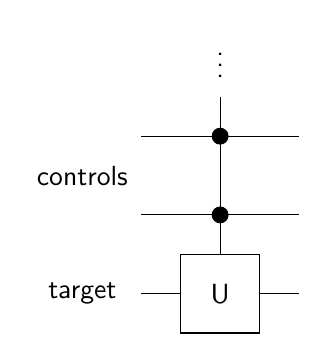
\begin{tikzpicture}[scale=.5] \node[draw=none] at (-3.5, 3) {controls}; \node[draw=none] at (-3.5, 0) {target}; \node[draw=none] at (0, 6) {$\vdots$}; \draw (0, 5) -- (0, 4); \draw (-2, 4) -- (2, 4); \draw[fill=black] (0, 4) circle (.2); \draw (0, 4) -- (0, 2); \draw (-2, 2) -- (2, 2); \draw[fill=black] (0, 2) circle (.2); \draw (0, 2) -- (0, 1); \draw (-2,0) -- (-1, 0); \draw (1, 0) -- (2, 0); \draw (-1,-1)--(-1,1)--(1,1)--(1,-1)--cycle; \node[draw=none] at (0, 0) {U}; \end{tikzpicture} } \]


\begin{DoxyParams}[1]{Parameters}
\mbox{\tt in,out}  & {\em multi\+Qubit} & object representing the set of all qubits \\
\hline
\mbox{\tt in}  & {\em control\+Qubits} & applies unitary if all qubits in this array equal 1 \\
\hline
\mbox{\tt in}  & {\em num\+Control\+Qubits} & number of control qubits \\
\hline
\mbox{\tt in}  & {\em target\+Qubit} & qubit to operate on \\
\hline
\mbox{\tt in}  & {\em u} & single-\/qubit unitary matrix to apply \\
\hline
\end{DoxyParams}

\begin{DoxyExceptions}{Exceptions}
{\em exit\+With\+Error} & if {\ttfamily num\+Control\+Qubits} is outside \mbox{[}1, {\ttfamily multi\+Qubit.\+num\+Qubits}\mbox{]}), or if any qubit index ({\ttfamily target\+Qubit} or one in {\ttfamily control\+Qubits}) is outside \mbox{[}0, {\ttfamily multi\+Qubit.\+num\+Qubits}\mbox{]}), or if {\ttfamily control\+Qubits} contains {\ttfamily target\+Qubit}, or if {\ttfamily u} is not unitary. \\
\hline
\end{DoxyExceptions}
\mbox{\Hypertarget{QuEST_8h_aedb5ef39da69e7895d714980dc621261}\label{QuEST_8h_aedb5ef39da69e7895d714980dc621261}} 
\index{Qu\+E\+S\+T.\+h@{Qu\+E\+S\+T.\+h}!Qu\+E\+S\+T\+Seed\+Random@{Qu\+E\+S\+T\+Seed\+Random}}
\index{Qu\+E\+S\+T\+Seed\+Random@{Qu\+E\+S\+T\+Seed\+Random}!Qu\+E\+S\+T.\+h@{Qu\+E\+S\+T.\+h}}
\paragraph{\texorpdfstring{Qu\+E\+S\+T\+Seed\+Random()}{QuESTSeedRandom()}}
{\footnotesize\ttfamily void Qu\+E\+S\+T\+Seed\+Random (\begin{DoxyParamCaption}\item[{unsigned long int $\ast$}]{seed\+Array,  }\item[{int}]{num\+Seeds }\end{DoxyParamCaption})}



Seed the Mersenne Twister used for random number generation in the Qu\+E\+ST environment with a user defined seed. 

This function uses the mt19937 init\+\_\+by\+\_\+array function with num\+Seeds keys supplied by the user. Subsequent calls to mt19937 genrand functions will use this seeding. For a multi process code, the same seed is given to all process, therefore this seeding is only appropriate to use for functions such as measure where all processes require the same random value.


\begin{DoxyParams}[1]{Parameters}
\mbox{\tt in}  & {\em seed\+Array} & Array of integers to use as seed. This allows the MT to be initialised with more than a 32-\/bit integer if required \\
\hline
\mbox{\tt in}  & {\em num\+Seeds} & Length of seed\+Array\\
\hline
\end{DoxyParams}
For more information about the MT, see \href{http://www.math.sci.hiroshima-u.ac.jp/~m-mat/MT/MT2002/emt19937ar.html}{\tt http\+://www.\+math.\+sci.\+hiroshima-\/u.\+ac.\+jp/$\sim$m-\/mat/\+M\+T/\+M\+T2002/emt19937ar.\+html}

Seed the Mersenne Twister used for random number generation in the Qu\+E\+ST environment with a user defined seed. 

Definition at line 231 of file Qu\+E\+S\+T.\+cpp.



References init\+\_\+by\+\_\+array().


\begin{DoxyCode}
231                                                                 \{
232     \textcolor{comment}{// init MT random number generator with user defined list of seeds}
233     \textcolor{comment}{// for the MPI version, it is ok that all procs will get the same seed as random numbers will only be }
234     \textcolor{comment}{// used by the master process}
235     \mbox{\hyperlink{mt19937ar_8cpp_ac1283f9b1ed571332f5ffe53545ffc16}{init\_by\_array}}(seedArray, numSeeds); 
236 \}
\end{DoxyCode}
\mbox{\Hypertarget{QuEST_8h_ac49f548ee27ae484695f9add1273adb4}\label{QuEST_8h_ac49f548ee27ae484695f9add1273adb4}} 
\index{Qu\+E\+S\+T.\+h@{Qu\+E\+S\+T.\+h}!Qu\+E\+S\+T\+Seed\+Random\+Default@{Qu\+E\+S\+T\+Seed\+Random\+Default}}
\index{Qu\+E\+S\+T\+Seed\+Random\+Default@{Qu\+E\+S\+T\+Seed\+Random\+Default}!Qu\+E\+S\+T.\+h@{Qu\+E\+S\+T.\+h}}
\paragraph{\texorpdfstring{Qu\+E\+S\+T\+Seed\+Random\+Default()}{QuESTSeedRandomDefault()}}
{\footnotesize\ttfamily void Qu\+E\+S\+T\+Seed\+Random\+Default (\begin{DoxyParamCaption}\item[{void}]{ }\end{DoxyParamCaption})}



Seed the Mersenne Twister used for random number generation in the Qu\+E\+ST environment with an example defualt seed. 

This default seeding function uses the mt19937 init\+\_\+by\+\_\+array function with three keys -- time, pid and hostname. Subsequent calls to mt19937 genrand functions will use this seeding. For a multi process code, the same seed is given to all process, therefore this seeding is only appropriate to use for functions such as measure where all processes require the same random value.

For more information about the MT, see \href{http://www.math.sci.hiroshima-u.ac.jp/~m-mat/MT/MT2002/emt19937ar.html}{\tt http\+://www.\+math.\+sci.\+hiroshima-\/u.\+ac.\+jp/$\sim$m-\/mat/\+M\+T/\+M\+T2002/emt19937ar.\+html} 

Definition at line 206 of file Qu\+E\+S\+T.\+cpp.



References hash\+String(), and init\+\_\+by\+\_\+array().


\begin{DoxyCode}
206                              \{
207     \textcolor{comment}{// init MT random number generator with three keys -- time, pid and a hash of hostname }
208     \textcolor{comment}{// for the MPI version, it is ok that all procs will get the same seed as random numbers will only be }
209     \textcolor{comment}{// used by the master process}
210 
211     \textcolor{keyword}{struct }timeval  tv;
212     gettimeofday(&tv, NULL);
213 
214     \textcolor{keywordtype}{double} time\_in\_mill = 
215         (tv.tv\_sec) * 1000 + (tv.tv\_usec) / 1000 ; \textcolor{comment}{// convert tv\_sec & tv\_usec to millisecond}
216 
217     \textcolor{keywordtype}{unsigned} \textcolor{keywordtype}{long} \textcolor{keywordtype}{int} pid = getpid();
218     \textcolor{keywordtype}{unsigned} \textcolor{keywordtype}{long} \textcolor{keywordtype}{int} msecs = (\textcolor{keywordtype}{unsigned} \textcolor{keywordtype}{long} int) time\_in\_mill;
219     \textcolor{keywordtype}{char} hostName[MAXHOSTNAMELEN+1];
220     gethostname(hostName, \textcolor{keyword}{sizeof}(hostName));
221     \textcolor{keywordtype}{unsigned} \textcolor{keywordtype}{long} \textcolor{keywordtype}{int} hostNameInt = \mbox{\hyperlink{QuEST_8cpp_ab76254cfde16f0808476649507a1a2fc}{hashString}}(hostName);
222 
223     \textcolor{keywordtype}{unsigned} \textcolor{keywordtype}{long} \textcolor{keywordtype}{int} key[3];
224     key[0] = msecs; key[1] = pid; key[2] = hostNameInt;
225     \mbox{\hyperlink{mt19937ar_8cpp_ac1283f9b1ed571332f5ffe53545ffc16}{init\_by\_array}}(key, 3); 
226 \}
\end{DoxyCode}
\mbox{\Hypertarget{QuEST_8h_aa5e77e0e64f3a4a3d3f5cc7382bffcd9}\label{QuEST_8h_aa5e77e0e64f3a4a3d3f5cc7382bffcd9}} 
\index{Qu\+E\+S\+T.\+h@{Qu\+E\+S\+T.\+h}!report\+Multi\+Qubit\+Params@{report\+Multi\+Qubit\+Params}}
\index{report\+Multi\+Qubit\+Params@{report\+Multi\+Qubit\+Params}!Qu\+E\+S\+T.\+h@{Qu\+E\+S\+T.\+h}}
\paragraph{\texorpdfstring{report\+Multi\+Qubit\+Params()}{reportMultiQubitParams()}}
{\footnotesize\ttfamily void report\+Multi\+Qubit\+Params (\begin{DoxyParamCaption}\item[{\mbox{\hyperlink{structMultiQubit}{Multi\+Qubit}}}]{multi\+Qubit }\end{DoxyParamCaption})}



Report metainformation about a set of qubits\+: number of qubits, number of probability amplitudes. 


\begin{DoxyParams}[1]{Parameters}
\mbox{\tt in,out}  & {\em multi\+Qubit} & object representing the set of qubits \\
\hline
\mbox{\tt in}  & {\em env} & object representing the execution environment (local, multinode etc) \\
\hline
\end{DoxyParams}


Definition at line 80 of file Qu\+E\+S\+T.\+cpp.



References Multi\+Qubit\+::chunk\+Id, Multi\+Qubit\+::num\+Chunks, and Multi\+Qubit\+::num\+Qubits.


\begin{DoxyCode}
80                                                   \{
81         \textcolor{keywordtype}{long} \textcolor{keywordtype}{long} \textcolor{keywordtype}{int} numAmps = 1L << multiQubit.\mbox{\hyperlink{structMultiQubit_ab5b9795bdc6fb5855e1974dcbbaeb36f}{numQubits}};
82         \textcolor{keywordtype}{long} \textcolor{keywordtype}{long} \textcolor{keywordtype}{int} numAmpsPerRank = numAmps/multiQubit.\mbox{\hyperlink{structMultiQubit_acd43f2f57991709c9e94f73662c972b2}{numChunks}};
83         \textcolor{keywordflow}{if} (multiQubit.\mbox{\hyperlink{structMultiQubit_ab10c88249fa3825d6227ceec01d37e37}{chunkId}}==0)\{
84                 printf(\textcolor{stringliteral}{"QUBITS:\(\backslash\)n"});
85                 printf(\textcolor{stringliteral}{"Number of qubits is %d.\(\backslash\)n"}, multiQubit.\mbox{\hyperlink{structMultiQubit_ab5b9795bdc6fb5855e1974dcbbaeb36f}{numQubits}});
86                 printf(\textcolor{stringliteral}{"Number of amps is %lld.\(\backslash\)n"}, numAmps);
87                 printf(\textcolor{stringliteral}{"Number of amps per rank is %lld.\(\backslash\)n"}, numAmpsPerRank);
88     \}
89 \}
\end{DoxyCode}
\mbox{\Hypertarget{QuEST_8h_af8a14ae79c3fb2c0b5f6255cc37bebf9}\label{QuEST_8h_af8a14ae79c3fb2c0b5f6255cc37bebf9}} 
\index{Qu\+E\+S\+T.\+h@{Qu\+E\+S\+T.\+h}!report\+Qu\+E\+S\+T\+Env@{report\+Qu\+E\+S\+T\+Env}}
\index{report\+Qu\+E\+S\+T\+Env@{report\+Qu\+E\+S\+T\+Env}!Qu\+E\+S\+T.\+h@{Qu\+E\+S\+T.\+h}}
\paragraph{\texorpdfstring{report\+Qu\+E\+S\+T\+Env()}{reportQuESTEnv()}}
{\footnotesize\ttfamily void report\+Qu\+E\+S\+T\+Env (\begin{DoxyParamCaption}\item[{\mbox{\hyperlink{structQuESTEnv}{Qu\+E\+S\+T\+Env}}}]{env }\end{DoxyParamCaption})}



Report information about the Qu\+E\+ST environment. 


\begin{DoxyParams}[1]{Parameters}
\mbox{\tt in}  & {\em env} & object representing the execution environment. A single instance is used for each program \\
\hline
\end{DoxyParams}
\mbox{\Hypertarget{QuEST_8h_a96f4de9ce7fefc7680a44d601fc3d894}\label{QuEST_8h_a96f4de9ce7fefc7680a44d601fc3d894}} 
\index{Qu\+E\+S\+T.\+h@{Qu\+E\+S\+T.\+h}!report\+State@{report\+State}}
\index{report\+State@{report\+State}!Qu\+E\+S\+T.\+h@{Qu\+E\+S\+T.\+h}}
\paragraph{\texorpdfstring{report\+State()}{reportState()}}
{\footnotesize\ttfamily void report\+State (\begin{DoxyParamCaption}\item[{\mbox{\hyperlink{structMultiQubit}{Multi\+Qubit}}}]{multi\+Qubit }\end{DoxyParamCaption})}



Print the current state vector of probability amplitudes for a set of qubits to file. 

File format\+: \begin{DoxyVerb}real, imag
realComponent1, imagComponent1
realComponent2, imagComponent2
...
realComponentN, imagComponentN
\end{DoxyVerb}


File naming convention\+:

For each node that the program runs on, a file \textquotesingle{}state\+\_\+rank\+\_\+\mbox{[}node\+\_\+rank\mbox{]}.csv\textquotesingle{} is generated. If there is more than one node, ranks after the first do not include the header \begin{DoxyVerb}real, imag
\end{DoxyVerb}
 so that files are easier to combine. 
\begin{DoxyParams}[1]{Parameters}
\mbox{\tt in,out}  & {\em multi\+Qubit} & object representing the set of qubits \\
\hline
\end{DoxyParams}


Definition at line 62 of file Qu\+E\+S\+T.\+cpp.



References Multi\+Qubit\+::chunk\+Id, Complex\+Array\+::imag, Multi\+Qubit\+::num\+Amps, Complex\+Array\+::real, and Multi\+Qubit\+::state\+Vec.


\begin{DoxyCode}
62                                        \{
63         FILE *state;
64         \textcolor{keywordtype}{char} filename[100];
65         \textcolor{keywordtype}{long} \textcolor{keywordtype}{long} \textcolor{keywordtype}{int} index;
66         sprintf(filename, \textcolor{stringliteral}{"state\_rank\_%d.csv"}, multiQubit.\mbox{\hyperlink{structMultiQubit_ab10c88249fa3825d6227ceec01d37e37}{chunkId}});
67         state = fopen(filename, \textcolor{stringliteral}{"w"});
68         \textcolor{keywordflow}{if} (multiQubit.\mbox{\hyperlink{structMultiQubit_ab10c88249fa3825d6227ceec01d37e37}{chunkId}}==0) fprintf(state, \textcolor{stringliteral}{"real, imag\(\backslash\)n"});
69 
70         \textcolor{keywordflow}{for}(index=0; index<multiQubit.\mbox{\hyperlink{structMultiQubit_ae16f47d8b725c914fb7f66b6498d79db}{numAmps}}; index++)\{
71                 fprintf(state, \textcolor{stringliteral}{"%.12f, %.12f\(\backslash\)n"}, multiQubit.\mbox{\hyperlink{structMultiQubit_a45483190d6b01ef6b2f98f2bec9ab94f}{stateVec}}.
      \mbox{\hyperlink{structComplexArray_a4195cac6c784ea1b6271f1c7dba1548a}{real}}[index], multiQubit.\mbox{\hyperlink{structMultiQubit_a45483190d6b01ef6b2f98f2bec9ab94f}{stateVec}}.\mbox{\hyperlink{structComplexArray_a79dde47c7ae530c79cebfdf57b225968}{imag}}[index]);
72         \}
73         fclose(state);
74 \}
\end{DoxyCode}
\mbox{\Hypertarget{QuEST_8h_a842d6884e063a5865a2232cba56b65ac}\label{QuEST_8h_a842d6884e063a5865a2232cba56b65ac}} 
\index{Qu\+E\+S\+T.\+h@{Qu\+E\+S\+T.\+h}!report\+State\+To\+Screen@{report\+State\+To\+Screen}}
\index{report\+State\+To\+Screen@{report\+State\+To\+Screen}!Qu\+E\+S\+T.\+h@{Qu\+E\+S\+T.\+h}}
\paragraph{\texorpdfstring{report\+State\+To\+Screen()}{reportStateToScreen()}}
{\footnotesize\ttfamily void report\+State\+To\+Screen (\begin{DoxyParamCaption}\item[{\mbox{\hyperlink{structMultiQubit}{Multi\+Qubit}}}]{multi\+Qubit,  }\item[{\mbox{\hyperlink{structQuESTEnv}{Qu\+E\+S\+T\+Env}}}]{env,  }\item[{int}]{report\+Rank }\end{DoxyParamCaption})}



Print the current state vector of probability amplitudes for a set of qubits to standard out. 

For debugging purposes. Each rank should print output serially. Only print output for systems $<$= 5 qubits \mbox{\Hypertarget{QuEST_8h_a7fadb225fc385db789e844c87fcba9e1}\label{QuEST_8h_a7fadb225fc385db789e844c87fcba9e1}} 
\index{Qu\+E\+S\+T.\+h@{Qu\+E\+S\+T.\+h}!rotate\+Around\+Axis@{rotate\+Around\+Axis}}
\index{rotate\+Around\+Axis@{rotate\+Around\+Axis}!Qu\+E\+S\+T.\+h@{Qu\+E\+S\+T.\+h}}
\paragraph{\texorpdfstring{rotate\+Around\+Axis()}{rotateAroundAxis()}}
{\footnotesize\ttfamily void rotate\+Around\+Axis (\begin{DoxyParamCaption}\item[{\mbox{\hyperlink{structMultiQubit}{Multi\+Qubit}}}]{multi\+Qubit,  }\item[{const int}]{rot\+Qubit,  }\item[{\mbox{\hyperlink{QuEST__precision_8h_a4b654506f18b8bfd61ad2a29a7e38c25}{R\+E\+AL}}}]{angle,  }\item[{\mbox{\hyperlink{structVector}{Vector}}}]{unit\+Axis }\end{DoxyParamCaption})}



Rotate a single qubit by a given angle around a given vector on the Bloch-\/sphere. 


\begin{DoxyItemize}
\item The vector must not be zero (else an error is thrown), but needn\textquotesingle{}t be unit magnitude.
\end{DoxyItemize}


\begin{DoxyParams}[1]{Parameters}
\mbox{\tt in,out}  & {\em multi\+Qubit} & object representing the set of all qubits \\
\hline
\mbox{\tt in}  & {\em rot\+Qubit} & qubit to rotate \\
\hline
\mbox{\tt in}  & {\em angle} & angle by which to rotate in radians \\
\hline
\mbox{\tt in}  & {\em axis} & vector around which to rotate \\
\hline
\end{DoxyParams}

\begin{DoxyExceptions}{Exceptions}
{\em exit\+With\+Error} & if {\ttfamily rot\+Qubit} is outside \mbox{[}0, {\ttfamily multi\+Qubit.\+num\+Qubits}), or if {\ttfamily axis} is the zero vector \\
\hline
\end{DoxyExceptions}


Definition at line 91 of file Qu\+E\+S\+T.\+cpp.



References compact\+Unitary(), Complex\+::imag, Complex\+::real, Vector\+::x, Vector\+::y, and Vector\+::z.



Referenced by rotate\+X(), rotate\+Y(), and rotate\+Z().


\begin{DoxyCode}
91                                                                                          \{
92 
93     \textcolor{keywordtype}{double} mag = sqrt(pow(axis.x,2) + pow(axis.y,2) + pow(axis.z,2));
94     \mbox{\hyperlink{structVector}{Vector}} unitAxis = \{axis.\mbox{\hyperlink{structVector_aac7abe171ba4bada50ed72acba6259fc}{x}}/mag, axis.y/mag, axis.z/mag\};
95 
96     \mbox{\hyperlink{structComplex}{Complex}} alpha, beta;
97     alpha.\mbox{\hyperlink{structComplex_a479ad939835457595fcca3ca55c06283}{real}} = cos(angle/2.0);
98     alpha.\mbox{\hyperlink{structComplex_a1151948284b21c0052f203f23ab931d9}{imag}} = -sin(angle/2.0)*unitAxis.\mbox{\hyperlink{structVector_ad4e863651be7d6b7e2b28cd7445a0ccf}{z}};    
99     beta.\mbox{\hyperlink{structComplex_a479ad939835457595fcca3ca55c06283}{real}} = sin(angle/2.0)*unitAxis.\mbox{\hyperlink{structVector_a375ca805d4c808a53d7c4e0c737ae3de}{y}};
100     beta.\mbox{\hyperlink{structComplex_a1151948284b21c0052f203f23ab931d9}{imag}} = -sin(angle/2.0)*unitAxis.\mbox{\hyperlink{structVector_aac7abe171ba4bada50ed72acba6259fc}{x}};
101     \mbox{\hyperlink{QuEST_8h_ad13ae1902276195d0df106116e032aff}{compactUnitary}}(multiQubit, rotQubit, alpha, beta);
102 \}
\end{DoxyCode}
\mbox{\Hypertarget{QuEST_8h_a6cc7fa705a2f2e6b486b49c5589d5df5}\label{QuEST_8h_a6cc7fa705a2f2e6b486b49c5589d5df5}} 
\index{Qu\+E\+S\+T.\+h@{Qu\+E\+S\+T.\+h}!rotateX@{rotateX}}
\index{rotateX@{rotateX}!Qu\+E\+S\+T.\+h@{Qu\+E\+S\+T.\+h}}
\paragraph{\texorpdfstring{rotate\+X()}{rotateX()}}
{\footnotesize\ttfamily void rotateX (\begin{DoxyParamCaption}\item[{\mbox{\hyperlink{structMultiQubit}{Multi\+Qubit}}}]{multi\+Qubit,  }\item[{const int}]{rot\+Qubit,  }\item[{\mbox{\hyperlink{QuEST__precision_8h_a4b654506f18b8bfd61ad2a29a7e38c25}{R\+E\+AL}}}]{angle }\end{DoxyParamCaption})}



Rotate a single qubit by a given angle around the X-\/axis of the Bloch-\/sphere. 

For angle $\theta$, applies \[ \begin{pmatrix} \cos\theta/2 & -i \sin \theta/2\\ -i \sin \theta/2 & \cos \theta/2 \end{pmatrix} \]

\[ \setlength{\fboxrule}{0.01pt} \fbox{ 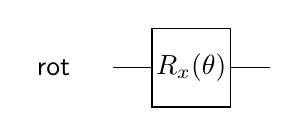
\begin{tikzpicture}[scale=.5] \node[draw=none] at (-3.5, 0) {rot}; \draw (-2,0) -- (-1, 0); \draw (1, 0) -- (2, 0); \draw (-1,-1)--(-1,1)--(1,1)--(1,-1)--cycle; \node[draw=none] at (0, 0) {$R_x(\theta)$}; \end{tikzpicture} } \]


\begin{DoxyParams}[1]{Parameters}
\mbox{\tt in,out}  & {\em multi\+Qubit} & object representing the set of all qubits \\
\hline
\mbox{\tt in}  & {\em rot\+Qubit} & qubit to rotate \\
\hline
\mbox{\tt in}  & {\em angle} & angle by which to rotate in radians \\
\hline
\end{DoxyParams}

\begin{DoxyExceptions}{Exceptions}
{\em exit\+With\+Error} & if {\ttfamily rot\+Qubit} is outside \mbox{[}0, {\ttfamily multi\+Qubit.\+num\+Qubits}). \\
\hline
\end{DoxyExceptions}


Definition at line 104 of file Qu\+E\+S\+T.\+cpp.



References rotate\+Around\+Axis().


\begin{DoxyCode}
104                                                                    \{
105 
106     \mbox{\hyperlink{structVector}{Vector}} unitAxis = \{1, 0, 0\};
107     \mbox{\hyperlink{QuEST_8cpp_a8810423457803005fecd415f4299f40d}{rotateAroundAxis}}(multiQubit, rotQubit, angle, unitAxis);
108 \}
\end{DoxyCode}
\mbox{\Hypertarget{QuEST_8h_ace0d3592d38a990e81a434c4e9681500}\label{QuEST_8h_ace0d3592d38a990e81a434c4e9681500}} 
\index{Qu\+E\+S\+T.\+h@{Qu\+E\+S\+T.\+h}!rotateY@{rotateY}}
\index{rotateY@{rotateY}!Qu\+E\+S\+T.\+h@{Qu\+E\+S\+T.\+h}}
\paragraph{\texorpdfstring{rotate\+Y()}{rotateY()}}
{\footnotesize\ttfamily void rotateY (\begin{DoxyParamCaption}\item[{\mbox{\hyperlink{structMultiQubit}{Multi\+Qubit}}}]{multi\+Qubit,  }\item[{const int}]{rot\+Qubit,  }\item[{\mbox{\hyperlink{QuEST__precision_8h_a4b654506f18b8bfd61ad2a29a7e38c25}{R\+E\+AL}}}]{angle }\end{DoxyParamCaption})}



Rotate a single qubit by a given angle around the Y-\/axis of the Bloch-\/sphere. 

For angle $\theta$, applies \[ \begin{pmatrix} \cos\theta/2 & \sin \theta/2\\ \sin \theta/2 & \cos \theta/2 \end{pmatrix} \] ~\newline
 \[ \setlength{\fboxrule}{0.01pt} \fbox{ 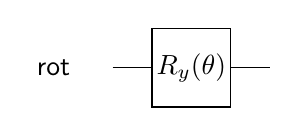
\begin{tikzpicture}[scale=.5] \node[draw=none] at (-3.5, 0) {rot}; \draw (-2,0) -- (-1, 0); \draw (1, 0) -- (2, 0); \draw (-1,-1)--(-1,1)--(1,1)--(1,-1)--cycle; \node[draw=none] at (0, 0) {$R_y(\theta)$}; \end{tikzpicture} } \]


\begin{DoxyParams}[1]{Parameters}
\mbox{\tt in,out}  & {\em multi\+Qubit} & object representing the set of all qubits \\
\hline
\mbox{\tt in}  & {\em rot\+Qubit} & qubit to rotate \\
\hline
\mbox{\tt in}  & {\em angle} & angle by which to rotate in radians \\
\hline
\end{DoxyParams}

\begin{DoxyExceptions}{Exceptions}
{\em exit\+With\+Error} & if {\ttfamily rot\+Qubit} is outside \mbox{[}0, {\ttfamily multi\+Qubit.\+num\+Qubits}). \\
\hline
\end{DoxyExceptions}


Definition at line 110 of file Qu\+E\+S\+T.\+cpp.



References rotate\+Around\+Axis().


\begin{DoxyCode}
110                                                                    \{
111 
112     \mbox{\hyperlink{structVector}{Vector}} unitAxis = \{0, 1, 0\};
113     \mbox{\hyperlink{QuEST_8cpp_a8810423457803005fecd415f4299f40d}{rotateAroundAxis}}(multiQubit, rotQubit, angle, unitAxis);
114 \}
\end{DoxyCode}
\mbox{\Hypertarget{QuEST_8h_abd621412ad30c1b034f4ce153c4afe10}\label{QuEST_8h_abd621412ad30c1b034f4ce153c4afe10}} 
\index{Qu\+E\+S\+T.\+h@{Qu\+E\+S\+T.\+h}!rotateZ@{rotateZ}}
\index{rotateZ@{rotateZ}!Qu\+E\+S\+T.\+h@{Qu\+E\+S\+T.\+h}}
\paragraph{\texorpdfstring{rotate\+Z()}{rotateZ()}}
{\footnotesize\ttfamily void rotateZ (\begin{DoxyParamCaption}\item[{\mbox{\hyperlink{structMultiQubit}{Multi\+Qubit}}}]{multi\+Qubit,  }\item[{const int}]{rot\+Qubit,  }\item[{\mbox{\hyperlink{QuEST__precision_8h_a4b654506f18b8bfd61ad2a29a7e38c25}{R\+E\+AL}}}]{angle }\end{DoxyParamCaption})}



Rotate a single qubit by a given angle around the Z-\/axis of the Bloch-\/sphere (also known as a phase shift gate). 

For angle $\theta$, applies \[ \begin{pmatrix} \exp(-i \theta/2) & 0 \\ 0 & \exp(i \theta/2) \end{pmatrix} \]

\[ \setlength{\fboxrule}{0.01pt} \fbox{ 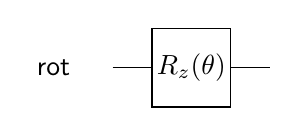
\begin{tikzpicture}[scale=.5] \node[draw=none] at (-3.5, 0) {rot}; \draw (-2,0) -- (-1, 0); \draw (1, 0) -- (2, 0); \draw (-1,-1)--(-1,1)--(1,1)--(1,-1)--cycle; \node[draw=none] at (0, 0) {$R_z(\theta)$}; \end{tikzpicture} } \]


\begin{DoxyParams}[1]{Parameters}
\mbox{\tt in,out}  & {\em multi\+Qubit} & object representing the set of all qubits \\
\hline
\mbox{\tt in}  & {\em rot\+Qubit} & qubit to rotate \\
\hline
\mbox{\tt in}  & {\em angle} & angle by which to rotate in radians \\
\hline
\end{DoxyParams}

\begin{DoxyExceptions}{Exceptions}
{\em exit\+With\+Error} & if {\ttfamily rot\+Qubit} is outside \mbox{[}0, {\ttfamily multi\+Qubit.\+num\+Qubits}). \\
\hline
\end{DoxyExceptions}


Definition at line 116 of file Qu\+E\+S\+T.\+cpp.



References rotate\+Around\+Axis().


\begin{DoxyCode}
116                                                                    \{
117 
118     \mbox{\hyperlink{structVector}{Vector}} unitAxis = \{0, 0, 1\};
119     \mbox{\hyperlink{QuEST_8cpp_a8810423457803005fecd415f4299f40d}{rotateAroundAxis}}(multiQubit, rotQubit, angle, unitAxis);
120 \}
\end{DoxyCode}
\mbox{\Hypertarget{QuEST_8h_adda6c47876a7676488ed0565a19eaa65}\label{QuEST_8h_adda6c47876a7676488ed0565a19eaa65}} 
\index{Qu\+E\+S\+T.\+h@{Qu\+E\+S\+T.\+h}!s\+Gate@{s\+Gate}}
\index{s\+Gate@{s\+Gate}!Qu\+E\+S\+T.\+h@{Qu\+E\+S\+T.\+h}}
\paragraph{\texorpdfstring{s\+Gate()}{sGate()}}
{\footnotesize\ttfamily void s\+Gate (\begin{DoxyParamCaption}\item[{\mbox{\hyperlink{structMultiQubit}{Multi\+Qubit}}}]{multi\+Qubit,  }\item[{const int}]{target\+Qubit }\end{DoxyParamCaption})}



Apply the single-\/qubit S gate. 

This is a rotation of $\pi/2$ around the Z-\/axis on the Bloch sphere, or the unitary\+: \[ \begin{pmatrix} 1 & 0 \\ 0 & i \end{pmatrix} \]

\[ \setlength{\fboxrule}{0.01pt} \fbox{ 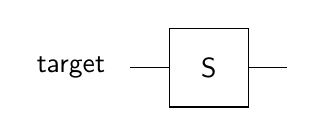
\begin{tikzpicture}[scale=.5] \node[draw=none] at (-3.5, 0) {target}; \draw (-2,0) -- (-1, 0); \draw (1, 0) -- (2, 0); \draw (-1,-1)--(-1,1)--(1,1)--(1,-1)--cycle; \node[draw=none] at (0, 0) {S}; \end{tikzpicture} } \]


\begin{DoxyParams}[1]{Parameters}
\mbox{\tt in,out}  & {\em multi\+Qubit} & object representing the set of all qubits \\
\hline
\mbox{\tt in}  & {\em target\+Qubit} & qubit to operate upon \\
\hline
\end{DoxyParams}

\begin{DoxyExceptions}{Exceptions}
{\em exit\+With\+Error} & if {\ttfamily target\+Qubit} is outside \mbox{[}0, {\ttfamily multi\+Qubit.\+num\+Qubits}) \\
\hline
\end{DoxyExceptions}


Definition at line 158 of file Qu\+E\+S\+T.\+cpp.



References phase\+Gate(), and S\+\_\+\+G\+A\+TE.


\begin{DoxyCode}
159 \{
160     \mbox{\hyperlink{QuEST__internal_8h_aae7a8a7f1ccbddb7f76b6c52b746bb43}{phaseGate}}(multiQubit, targetQubit, \mbox{\hyperlink{QuEST_8h_a5739021c733cecc49647956b2f7338eaa06e60f80fa80cce271793d6d31bcc21f}{S\_GATE}});
161 \} 
\end{DoxyCode}
\mbox{\Hypertarget{QuEST_8h_a86e396e06b7d527cac20ba0108872423}\label{QuEST_8h_a86e396e06b7d527cac20ba0108872423}} 
\index{Qu\+E\+S\+T.\+h@{Qu\+E\+S\+T.\+h}!sigmaX@{sigmaX}}
\index{sigmaX@{sigmaX}!Qu\+E\+S\+T.\+h@{Qu\+E\+S\+T.\+h}}
\paragraph{\texorpdfstring{sigma\+X()}{sigmaX()}}
{\footnotesize\ttfamily void sigmaX (\begin{DoxyParamCaption}\item[{\mbox{\hyperlink{structMultiQubit}{Multi\+Qubit}}}]{multi\+Qubit,  }\item[{const int}]{target\+Qubit }\end{DoxyParamCaption})}



Apply the single-\/qubit sigma-\/X (also known as the X, Pauli-\/X, N\+OT or bit-\/flip) gate. 

This is a rotation of $\pi$ around the x-\/axis on the Bloch sphere. I.\+e. \[ \begin{pmatrix} 0 & 1 \\ 1 & 0 \end{pmatrix} \] ~\newline
 \[ \setlength{\fboxrule}{0.01pt} \fbox{ 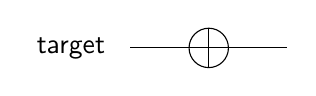
\begin{tikzpicture}[scale=.5] \node[draw=none] at (-3.5, 0) {target}; \draw (-2,0) -- (2, 0); \draw (0, 0) circle (.5); \draw (0, .5) -- (0, -.5); \end{tikzpicture} } \] ~\newline
 
\begin{DoxyParams}[1]{Parameters}
\mbox{\tt in,out}  & {\em multi\+Qubit} & object representing the set of all qubits \\
\hline
\mbox{\tt in}  & {\em target\+Qubit} & qubit to operate on \\
\hline
\end{DoxyParams}

\begin{DoxyExceptions}{Exceptions}
{\em exit\+With\+Error} & if {\ttfamily target\+Qubit} is outside \mbox{[}0, {\ttfamily multi\+Qubit.\+num\+Qubits}). \\
\hline
\end{DoxyExceptions}
\mbox{\Hypertarget{QuEST_8h_a1f54d70a42403f7e1c2e2c2007332f61}\label{QuEST_8h_a1f54d70a42403f7e1c2e2c2007332f61}} 
\index{Qu\+E\+S\+T.\+h@{Qu\+E\+S\+T.\+h}!sigmaY@{sigmaY}}
\index{sigmaY@{sigmaY}!Qu\+E\+S\+T.\+h@{Qu\+E\+S\+T.\+h}}
\paragraph{\texorpdfstring{sigma\+Y()}{sigmaY()}}
{\footnotesize\ttfamily void sigmaY (\begin{DoxyParamCaption}\item[{\mbox{\hyperlink{structMultiQubit}{Multi\+Qubit}}}]{multi\+Qubit,  }\item[{const int}]{target\+Qubit }\end{DoxyParamCaption})}



Apply the single-\/qubit sigma-\/Y (also known as the Y or Pauli-\/Y) gate. 

This is a rotation of $\pi$ around the Y-\/axis on the Bloch sphere. I.\+e. \[ \begin{pmatrix} 0 & -i \\ i & 0 \end{pmatrix} \] ~\newline
 \[ \setlength{\fboxrule}{0.01pt} \fbox{ 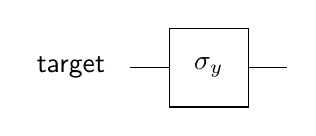
\begin{tikzpicture}[scale=.5] \node[draw=none] at (-3.5, 0) {target}; \draw (-2,0) -- (-1, 0); \draw (1, 0) -- (2, 0); \draw (-1,-1)--(-1,1)--(1,1)--(1,-1)--cycle; \node[draw=none] at (0, 0) {$\sigma_y$}; \end{tikzpicture} } \] ~\newline
 
\begin{DoxyParams}[1]{Parameters}
\mbox{\tt in,out}  & {\em multi\+Qubit} & object representing the set of all qubits \\
\hline
\mbox{\tt in}  & {\em target\+Qubit} & qubit to operate on \\
\hline
\end{DoxyParams}

\begin{DoxyExceptions}{Exceptions}
{\em exit\+With\+Error} & if {\ttfamily target\+Qubit} is outside \mbox{[}0, {\ttfamily multi\+Qubit.\+num\+Qubits}). \\
\hline
\end{DoxyExceptions}
\mbox{\Hypertarget{QuEST_8h_aebaab86326779de55d335cfea3efde8f}\label{QuEST_8h_aebaab86326779de55d335cfea3efde8f}} 
\index{Qu\+E\+S\+T.\+h@{Qu\+E\+S\+T.\+h}!sigmaZ@{sigmaZ}}
\index{sigmaZ@{sigmaZ}!Qu\+E\+S\+T.\+h@{Qu\+E\+S\+T.\+h}}
\paragraph{\texorpdfstring{sigma\+Z()}{sigmaZ()}}
{\footnotesize\ttfamily void sigmaZ (\begin{DoxyParamCaption}\item[{\mbox{\hyperlink{structMultiQubit}{Multi\+Qubit}}}]{multi\+Qubit,  }\item[{const int}]{target\+Qubit }\end{DoxyParamCaption})}



Apply the single-\/qubit sigma-\/Z (also known as the Z, Pauli-\/Z or phase-\/flip) gate. 

This is a rotation of $\pi$ around the Z-\/axis (a phase shift) on the Bloch sphere. I.\+e. \[ \begin{pmatrix} 1 & 0 \\ 0 & -1 \end{pmatrix} \] ~\newline
 \[ \setlength{\fboxrule}{0.01pt} \fbox{ 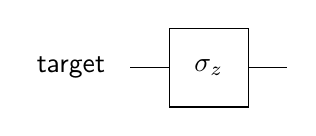
\begin{tikzpicture}[scale=.5] \node[draw=none] at (-3.5, 0) {target}; \draw (-2,0) -- (-1, 0); \draw (1, 0) -- (2, 0); \draw (-1,-1)--(-1,1)--(1,1)--(1,-1)--cycle; \node[draw=none] at (0, 0) {$\sigma_z$}; \end{tikzpicture} } \] ~\newline
 
\begin{DoxyParams}[1]{Parameters}
\mbox{\tt in,out}  & {\em multi\+Qubit} & object representing the set of all qubits \\
\hline
\mbox{\tt in}  & {\em target\+Qubit} & qubit to operate on \\
\hline
\end{DoxyParams}

\begin{DoxyExceptions}{Exceptions}
{\em exit\+With\+Error} & if {\ttfamily target\+Qubit} is outside \mbox{[}0, {\ttfamily multi\+Qubit.\+num\+Qubits}). \\
\hline
\end{DoxyExceptions}


Definition at line 153 of file Qu\+E\+S\+T.\+cpp.



References phase\+Gate(), and S\+I\+G\+M\+A\+\_\+Z.


\begin{DoxyCode}
154 \{
155     \mbox{\hyperlink{QuEST__internal_8h_aae7a8a7f1ccbddb7f76b6c52b746bb43}{phaseGate}}(multiQubit, targetQubit, \mbox{\hyperlink{QuEST_8h_a5739021c733cecc49647956b2f7338eaa754922d1e1846a1961ff2bf163483dac}{SIGMA\_Z}});
156 \}
\end{DoxyCode}
\mbox{\Hypertarget{QuEST_8h_a8d31fe2d1ad4d01e2a1f5f6b8bc15b77}\label{QuEST_8h_a8d31fe2d1ad4d01e2a1f5f6b8bc15b77}} 
\index{Qu\+E\+S\+T.\+h@{Qu\+E\+S\+T.\+h}!sync\+Qu\+E\+S\+T\+Env@{sync\+Qu\+E\+S\+T\+Env}}
\index{sync\+Qu\+E\+S\+T\+Env@{sync\+Qu\+E\+S\+T\+Env}!Qu\+E\+S\+T.\+h@{Qu\+E\+S\+T.\+h}}
\paragraph{\texorpdfstring{sync\+Qu\+E\+S\+T\+Env()}{syncQuESTEnv()}}
{\footnotesize\ttfamily void sync\+Qu\+E\+S\+T\+Env (\begin{DoxyParamCaption}\item[{\mbox{\hyperlink{structQuESTEnv}{Qu\+E\+S\+T\+Env}}}]{env }\end{DoxyParamCaption})}



Guarantees that all code up to the given point has been executed on all nodes. 


\begin{DoxyParams}[1]{Parameters}
\mbox{\tt in}  & {\em env} & object representing the execution environment. A single instance is used for each program \\
\hline
\end{DoxyParams}
\mbox{\Hypertarget{QuEST_8h_ac7e38d768a1bd79019f88cc1e6295092}\label{QuEST_8h_ac7e38d768a1bd79019f88cc1e6295092}} 
\index{Qu\+E\+S\+T.\+h@{Qu\+E\+S\+T.\+h}!sync\+Qu\+E\+S\+T\+Success@{sync\+Qu\+E\+S\+T\+Success}}
\index{sync\+Qu\+E\+S\+T\+Success@{sync\+Qu\+E\+S\+T\+Success}!Qu\+E\+S\+T.\+h@{Qu\+E\+S\+T.\+h}}
\paragraph{\texorpdfstring{sync\+Qu\+E\+S\+T\+Success()}{syncQuESTSuccess()}}
{\footnotesize\ttfamily int sync\+Qu\+E\+S\+T\+Success (\begin{DoxyParamCaption}\item[{int}]{success\+Code }\end{DoxyParamCaption})}



Performs a logical A\+ND on all success\+Codes held by all processes. 

If any one process has a zero success\+Code all processes will return a zero success code.


\begin{DoxyParams}[1]{Parameters}
\mbox{\tt in}  & {\em env} & object representing the execution environment. A single instance is used for each program \\
\hline
\mbox{\tt in}  & {\em success\+Code} & 1 if process task succeeded, 0 if process task failed \\
\hline
\end{DoxyParams}
\begin{DoxyReturn}{Returns}
1 if all processes succeeded, 0 if any one process failed 
\end{DoxyReturn}
\mbox{\Hypertarget{QuEST_8h_af764ea63a2e870098f4e1ce08562942e}\label{QuEST_8h_af764ea63a2e870098f4e1ce08562942e}} 
\index{Qu\+E\+S\+T.\+h@{Qu\+E\+S\+T.\+h}!t\+Gate@{t\+Gate}}
\index{t\+Gate@{t\+Gate}!Qu\+E\+S\+T.\+h@{Qu\+E\+S\+T.\+h}}
\paragraph{\texorpdfstring{t\+Gate()}{tGate()}}
{\footnotesize\ttfamily void t\+Gate (\begin{DoxyParamCaption}\item[{\mbox{\hyperlink{structMultiQubit}{Multi\+Qubit}}}]{multi\+Qubit,  }\item[{const int}]{target\+Qubit }\end{DoxyParamCaption})}



Apply the single-\/qubit T gate. 

This is a rotation of $\pi/4$ around the Z-\/axis on the Bloch sphere, or the unitary\+: \[ \begin{pmatrix} 1 & 0 \\ 0 & \exp\left(i \frac{\pi}{4}\right) \end{pmatrix} \]

\[ \setlength{\fboxrule}{0.01pt} \fbox{ 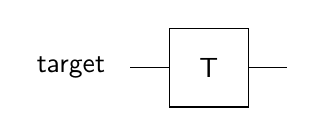
\begin{tikzpicture}[scale=.5] \node[draw=none] at (-3.5, 0) {target}; \draw (-2,0) -- (-1, 0); \draw (1, 0) -- (2, 0); \draw (-1,-1)--(-1,1)--(1,1)--(1,-1)--cycle; \node[draw=none] at (0, 0) {T}; \end{tikzpicture} } \]


\begin{DoxyParams}[1]{Parameters}
\mbox{\tt in,out}  & {\em multi\+Qubit} & object representing the set of all qubits \\
\hline
\mbox{\tt in}  & {\em target\+Qubit} & qubit to operate upon \\
\hline
\end{DoxyParams}

\begin{DoxyExceptions}{Exceptions}
{\em exit\+With\+Error} & if {\ttfamily target\+Qubit} is outside \mbox{[}0, {\ttfamily multi\+Qubit.\+num\+Qubits}) \\
\hline
\end{DoxyExceptions}


Definition at line 163 of file Qu\+E\+S\+T.\+cpp.



References phase\+Gate(), and T\+\_\+\+G\+A\+TE.


\begin{DoxyCode}
164 \{
165     \mbox{\hyperlink{QuEST__internal_8h_aae7a8a7f1ccbddb7f76b6c52b746bb43}{phaseGate}}(multiQubit, targetQubit, \mbox{\hyperlink{QuEST_8h_a5739021c733cecc49647956b2f7338eaa614d07d597a8e320cc556bc0e652e4ab}{T\_GATE}});
166 \}
\end{DoxyCode}
\mbox{\Hypertarget{QuEST_8h_a7a0877e33700f6bad48adb51b7b3fb67}\label{QuEST_8h_a7a0877e33700f6bad48adb51b7b3fb67}} 
\index{Qu\+E\+S\+T.\+h@{Qu\+E\+S\+T.\+h}!unitary@{unitary}}
\index{unitary@{unitary}!Qu\+E\+S\+T.\+h@{Qu\+E\+S\+T.\+h}}
\paragraph{\texorpdfstring{unitary()}{unitary()}}
{\footnotesize\ttfamily void unitary (\begin{DoxyParamCaption}\item[{\mbox{\hyperlink{structMultiQubit}{Multi\+Qubit}}}]{multi\+Qubit,  }\item[{const int}]{target\+Qubit,  }\item[{\mbox{\hyperlink{structComplexMatrix2}{Complex\+Matrix2}}}]{u }\end{DoxyParamCaption})}



Apply a general single-\/qubit unitary (including a global phase factor). 

The passed 2x2 Complex\+Matrix must be unitary, otherwise an error is thrown.

\[ \setlength{\fboxrule}{0.01pt} \fbox{ 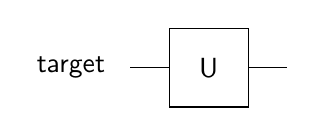
\begin{tikzpicture}[scale=.5] \node[draw=none] at (-3.5, 0) {target}; \draw (-2,0) -- (-1, 0); \draw (1, 0) -- (2, 0); \draw (-1,-1)--(-1,1)--(1,1)--(1,-1)--cycle; \node[draw=none] at (0, 0) {U}; \end{tikzpicture} } \]


\begin{DoxyParams}[1]{Parameters}
\mbox{\tt in,out}  & {\em multi\+Qubit} & object representing the set of all qubits \\
\hline
\mbox{\tt in}  & {\em target\+Qubit} & qubit to operate on \\
\hline
\mbox{\tt in}  & {\em u} & unitary matrix to apply \\
\hline
\end{DoxyParams}

\begin{DoxyExceptions}{Exceptions}
{\em exit\+With\+Error} & if {\ttfamily target\+Qubit} is outside \mbox{[}0, {\ttfamily multi\+Qubit.\+num\+Qubits}), or matrix {\ttfamily u} is not unitary. \\
\hline
\end{DoxyExceptions}

\hypertarget{QuEST__debug_8h}{}\subsection{Qu\+E\+S\+T\+\_\+debug.\+h File Reference}
\label{QuEST__debug_8h}\index{Qu\+E\+S\+T\+\_\+debug.\+h@{Qu\+E\+S\+T\+\_\+debug.\+h}}


Developer functions used for unit testing and debugging.  


{\ttfamily \#include \char`\"{}Qu\+E\+S\+T\+\_\+precision.\+h\char`\"{}}\newline
\subsubsection*{Functions}
\begin{DoxyCompactItemize}
\item 
void \mbox{\hyperlink{QuEST__debug_8h_a7169fd0442cbc3418f3fac4d13363ca2}{init\+State\+Of\+Single\+Qubit}} (\mbox{\hyperlink{structMultiQubit}{Multi\+Qubit}} $\ast$multi\+Qubit, int qubit\+Id, int outcome)
\item 
void \mbox{\hyperlink{QuEST__debug_8h_a03b3577a891731d505bc4b879fcca9d3}{init\+State\+Debug}} (\mbox{\hyperlink{structMultiQubit}{Multi\+Qubit}} $\ast$multi\+Qubit)
\item 
void \mbox{\hyperlink{QuEST__debug_8h_a433876ee9f3bcc54af346300f571fc3c}{initialize\+State\+From\+Single\+File}} (\mbox{\hyperlink{structMultiQubit}{Multi\+Qubit}} $\ast$multi\+Qubit, char filename\mbox{[}200\mbox{]}, \mbox{\hyperlink{structQuESTEnv}{Qu\+E\+S\+T\+Env}} env)
\item 
int \mbox{\hyperlink{QuEST__debug_8h_a793584932ae384c82e7e42db7d35d18d}{compare\+States}} (\mbox{\hyperlink{structMultiQubit}{Multi\+Qubit}} mq1, \mbox{\hyperlink{structMultiQubit}{Multi\+Qubit}} mq2, \mbox{\hyperlink{QuEST__precision_8h_a4b654506f18b8bfd61ad2a29a7e38c25}{R\+E\+AL}} precision)
\item 
void \mbox{\hyperlink{QuEST__debug_8h_a62da5b58d8ce84e6f4d24be1b872294e}{report\+Node\+List}} (\mbox{\hyperlink{structQuESTEnv}{Qu\+E\+S\+T\+Env}} env)
\begin{DoxyCompactList}\small\item\em Report a list of C\+PU hostnames and the rank that is running on each if running with M\+PI enabled and an error message otherwise. \end{DoxyCompactList}\end{DoxyCompactItemize}


\subsubsection{Detailed Description}
Developer functions used for unit testing and debugging. 

Not part of the public A\+PI. May contain functions that are incomplete or untested. 

\subsubsection{Function Documentation}
\mbox{\Hypertarget{QuEST__debug_8h_a793584932ae384c82e7e42db7d35d18d}\label{QuEST__debug_8h_a793584932ae384c82e7e42db7d35d18d}} 
\index{Qu\+E\+S\+T\+\_\+debug.\+h@{Qu\+E\+S\+T\+\_\+debug.\+h}!compare\+States@{compare\+States}}
\index{compare\+States@{compare\+States}!Qu\+E\+S\+T\+\_\+debug.\+h@{Qu\+E\+S\+T\+\_\+debug.\+h}}
\paragraph{\texorpdfstring{compare\+States()}{compareStates()}}
{\footnotesize\ttfamily int compare\+States (\begin{DoxyParamCaption}\item[{\mbox{\hyperlink{structMultiQubit}{Multi\+Qubit}}}]{mq1,  }\item[{\mbox{\hyperlink{structMultiQubit}{Multi\+Qubit}}}]{mq2,  }\item[{\mbox{\hyperlink{QuEST__precision_8h_a4b654506f18b8bfd61ad2a29a7e38c25}{R\+E\+AL}}}]{precision }\end{DoxyParamCaption})}

\mbox{\Hypertarget{QuEST__debug_8h_a433876ee9f3bcc54af346300f571fc3c}\label{QuEST__debug_8h_a433876ee9f3bcc54af346300f571fc3c}} 
\index{Qu\+E\+S\+T\+\_\+debug.\+h@{Qu\+E\+S\+T\+\_\+debug.\+h}!initialize\+State\+From\+Single\+File@{initialize\+State\+From\+Single\+File}}
\index{initialize\+State\+From\+Single\+File@{initialize\+State\+From\+Single\+File}!Qu\+E\+S\+T\+\_\+debug.\+h@{Qu\+E\+S\+T\+\_\+debug.\+h}}
\paragraph{\texorpdfstring{initialize\+State\+From\+Single\+File()}{initializeStateFromSingleFile()}}
{\footnotesize\ttfamily void initialize\+State\+From\+Single\+File (\begin{DoxyParamCaption}\item[{\mbox{\hyperlink{structMultiQubit}{Multi\+Qubit}} $\ast$}]{multi\+Qubit,  }\item[{char}]{filename\mbox{[}200\mbox{]},  }\item[{\mbox{\hyperlink{structQuESTEnv}{Qu\+E\+S\+T\+Env}}}]{env }\end{DoxyParamCaption})}

\mbox{\Hypertarget{QuEST__debug_8h_a03b3577a891731d505bc4b879fcca9d3}\label{QuEST__debug_8h_a03b3577a891731d505bc4b879fcca9d3}} 
\index{Qu\+E\+S\+T\+\_\+debug.\+h@{Qu\+E\+S\+T\+\_\+debug.\+h}!init\+State\+Debug@{init\+State\+Debug}}
\index{init\+State\+Debug@{init\+State\+Debug}!Qu\+E\+S\+T\+\_\+debug.\+h@{Qu\+E\+S\+T\+\_\+debug.\+h}}
\paragraph{\texorpdfstring{init\+State\+Debug()}{initStateDebug()}}
{\footnotesize\ttfamily void init\+State\+Debug (\begin{DoxyParamCaption}\item[{\mbox{\hyperlink{structMultiQubit}{Multi\+Qubit}} $\ast$}]{multi\+Qubit }\end{DoxyParamCaption})}

\mbox{\Hypertarget{QuEST__debug_8h_a7169fd0442cbc3418f3fac4d13363ca2}\label{QuEST__debug_8h_a7169fd0442cbc3418f3fac4d13363ca2}} 
\index{Qu\+E\+S\+T\+\_\+debug.\+h@{Qu\+E\+S\+T\+\_\+debug.\+h}!init\+State\+Of\+Single\+Qubit@{init\+State\+Of\+Single\+Qubit}}
\index{init\+State\+Of\+Single\+Qubit@{init\+State\+Of\+Single\+Qubit}!Qu\+E\+S\+T\+\_\+debug.\+h@{Qu\+E\+S\+T\+\_\+debug.\+h}}
\paragraph{\texorpdfstring{init\+State\+Of\+Single\+Qubit()}{initStateOfSingleQubit()}}
{\footnotesize\ttfamily void init\+State\+Of\+Single\+Qubit (\begin{DoxyParamCaption}\item[{\mbox{\hyperlink{structMultiQubit}{Multi\+Qubit}} $\ast$}]{multi\+Qubit,  }\item[{int}]{qubit\+Id,  }\item[{int}]{outcome }\end{DoxyParamCaption})}

\mbox{\Hypertarget{QuEST__debug_8h_a62da5b58d8ce84e6f4d24be1b872294e}\label{QuEST__debug_8h_a62da5b58d8ce84e6f4d24be1b872294e}} 
\index{Qu\+E\+S\+T\+\_\+debug.\+h@{Qu\+E\+S\+T\+\_\+debug.\+h}!report\+Node\+List@{report\+Node\+List}}
\index{report\+Node\+List@{report\+Node\+List}!Qu\+E\+S\+T\+\_\+debug.\+h@{Qu\+E\+S\+T\+\_\+debug.\+h}}
\paragraph{\texorpdfstring{report\+Node\+List()}{reportNodeList()}}
{\footnotesize\ttfamily void report\+Node\+List (\begin{DoxyParamCaption}\item[{\mbox{\hyperlink{structQuESTEnv}{Qu\+E\+S\+T\+Env}}}]{env }\end{DoxyParamCaption})}



Report a list of C\+PU hostnames and the rank that is running on each if running with M\+PI enabled and an error message otherwise. 

For debugging purposes. 
\begin{DoxyParams}[1]{Parameters}
\mbox{\tt in}  & {\em env} & object representing the execution environment. A single instance is used for each program \\
\hline
\end{DoxyParams}

\hypertarget{QuEST__internal_8h}{}\subsection{Qu\+E\+S\+T\+\_\+internal.\+h File Reference}
\label{QuEST__internal_8h}\index{Qu\+E\+S\+T\+\_\+internal.\+h@{Qu\+E\+S\+T\+\_\+internal.\+h}}


Internal functions used to implement the public facing A\+PI in qubits.\+h.  


{\ttfamily \#include \char`\"{}Qu\+E\+S\+T\+\_\+precision.\+h\char`\"{}}\newline
\subsubsection*{Functions}
\begin{DoxyCompactItemize}
\item 
void \mbox{\hyperlink{QuEST__internal_8h_aae7a8a7f1ccbddb7f76b6c52b746bb43}{phase\+Gate}} (\mbox{\hyperlink{structMultiQubit}{Multi\+Qubit}} multi\+Qubit, const int target\+Qubit, enum \mbox{\hyperlink{QuEST_8h_a5739021c733cecc49647956b2f7338ea}{phase\+Gate\+Type}} type)
\item 
\mbox{\hyperlink{QuEST__precision_8h_a4b654506f18b8bfd61ad2a29a7e38c25}{R\+E\+AL}} \mbox{\hyperlink{QuEST__internal_8h_a2e4cedb70bd181d250b3abb945cc108e}{find\+Probability\+Of\+Zero}} (\mbox{\hyperlink{structMultiQubit}{Multi\+Qubit}} multi\+Qubit, const int measure\+Qubit)
\begin{DoxyCompactList}\small\item\em Measure the probability of a specified qubit being in the zero state. \end{DoxyCompactList}\item 
\mbox{\hyperlink{QuEST__precision_8h_a4b654506f18b8bfd61ad2a29a7e38c25}{R\+E\+AL}} \mbox{\hyperlink{QuEST__internal_8h_a21094de735f3cb48488a184cfa4d8d41}{measure\+In\+Zero}} (\mbox{\hyperlink{structMultiQubit}{Multi\+Qubit}} multi\+Qubit, const int measure\+Qubit)
\begin{DoxyCompactList}\small\item\em Update the state vector to be consistent with measuring measure\+Qubit=0. \end{DoxyCompactList}\item 
int \mbox{\hyperlink{QuEST__internal_8h_ae4fea133d1a8f09ff8da03038100adb2}{validate\+Matrix\+Is\+Unitary}} (\mbox{\hyperlink{structComplexMatrix2}{Complex\+Matrix2}} u)
\item 
int \mbox{\hyperlink{QuEST__internal_8h_ae2b2c14a07dd7d50ff86032a3ca101d7}{validate\+Alpha\+Beta}} (\mbox{\hyperlink{structComplex}{Complex}} alpha, \mbox{\hyperlink{structComplex}{Complex}} beta)
\item 
int \mbox{\hyperlink{QuEST__internal_8h_a71c14976f63cfcda70026fa20ee531fe}{validate\+Unit\+Vector}} (\mbox{\hyperlink{QuEST__precision_8h_a4b654506f18b8bfd61ad2a29a7e38c25}{R\+E\+AL}} ux, \mbox{\hyperlink{QuEST__precision_8h_a4b654506f18b8bfd61ad2a29a7e38c25}{R\+E\+AL}} uy, \mbox{\hyperlink{QuEST__precision_8h_a4b654506f18b8bfd61ad2a29a7e38c25}{R\+E\+AL}} uz)
\item 
void \mbox{\hyperlink{QuEST__internal_8h_ae5f9019826f35e8b51b1716cfe397b45}{exit\+With\+Error}} (int error\+Code, const char $\ast$func)
\item 
void \mbox{\hyperlink{QuEST__internal_8h_a3587b9d533e633ccf1abf9ad2ce45d8d}{Qu\+E\+S\+T\+Assert}} (int is\+Valid, int error\+Code, const char $\ast$func)
\item 
unsigned long int \mbox{\hyperlink{QuEST__internal_8h_ab76254cfde16f0808476649507a1a2fc}{hash\+String}} (char $\ast$str)
\end{DoxyCompactItemize}
\subsubsection*{Variables}
\begin{DoxyCompactItemize}
\item 
const char $\ast$ \mbox{\hyperlink{QuEST__internal_8h_aac1637696885c75b73a1ecf381cea713}{error\+Codes}} \mbox{[}$\,$\mbox{]}
\end{DoxyCompactItemize}


\subsubsection{Detailed Description}
Internal functions used to implement the public facing A\+PI in qubits.\+h. 

Do not call these functions directly. 

\subsubsection{Function Documentation}
\mbox{\Hypertarget{QuEST__internal_8h_ae5f9019826f35e8b51b1716cfe397b45}\label{QuEST__internal_8h_ae5f9019826f35e8b51b1716cfe397b45}} 
\index{Qu\+E\+S\+T\+\_\+internal.\+h@{Qu\+E\+S\+T\+\_\+internal.\+h}!exit\+With\+Error@{exit\+With\+Error}}
\index{exit\+With\+Error@{exit\+With\+Error}!Qu\+E\+S\+T\+\_\+internal.\+h@{Qu\+E\+S\+T\+\_\+internal.\+h}}
\paragraph{\texorpdfstring{exit\+With\+Error()}{exitWithError()}}
{\footnotesize\ttfamily void exit\+With\+Error (\begin{DoxyParamCaption}\item[{int}]{error\+Code,  }\item[{const char $\ast$}]{func }\end{DoxyParamCaption})}

\mbox{\Hypertarget{QuEST__internal_8h_a2e4cedb70bd181d250b3abb945cc108e}\label{QuEST__internal_8h_a2e4cedb70bd181d250b3abb945cc108e}} 
\index{Qu\+E\+S\+T\+\_\+internal.\+h@{Qu\+E\+S\+T\+\_\+internal.\+h}!find\+Probability\+Of\+Zero@{find\+Probability\+Of\+Zero}}
\index{find\+Probability\+Of\+Zero@{find\+Probability\+Of\+Zero}!Qu\+E\+S\+T\+\_\+internal.\+h@{Qu\+E\+S\+T\+\_\+internal.\+h}}
\paragraph{\texorpdfstring{find\+Probability\+Of\+Zero()}{findProbabilityOfZero()}}
{\footnotesize\ttfamily \mbox{\hyperlink{QuEST__precision_8h_a4b654506f18b8bfd61ad2a29a7e38c25}{R\+E\+AL}} find\+Probability\+Of\+Zero (\begin{DoxyParamCaption}\item[{\mbox{\hyperlink{structMultiQubit}{Multi\+Qubit}}}]{multi\+Qubit,  }\item[{const int}]{measure\+Qubit }\end{DoxyParamCaption})}



Measure the probability of a specified qubit being in the zero state. 


\begin{DoxyParams}[1]{Parameters}
\mbox{\tt in}  & {\em multi\+Qubit} & object representing the set of qubits \\
\hline
\mbox{\tt in}  & {\em measure\+Qubit} & qubit to measure \\
\hline
\end{DoxyParams}
\begin{DoxyReturn}{Returns}
probability of qubit measure\+Qubit being zero 
\end{DoxyReturn}
\mbox{\Hypertarget{QuEST__internal_8h_ab76254cfde16f0808476649507a1a2fc}\label{QuEST__internal_8h_ab76254cfde16f0808476649507a1a2fc}} 
\index{Qu\+E\+S\+T\+\_\+internal.\+h@{Qu\+E\+S\+T\+\_\+internal.\+h}!hash\+String@{hash\+String}}
\index{hash\+String@{hash\+String}!Qu\+E\+S\+T\+\_\+internal.\+h@{Qu\+E\+S\+T\+\_\+internal.\+h}}
\paragraph{\texorpdfstring{hash\+String()}{hashString()}}
{\footnotesize\ttfamily unsigned long int hash\+String (\begin{DoxyParamCaption}\item[{char $\ast$}]{str }\end{DoxyParamCaption})}



Definition at line 238 of file Qu\+E\+S\+T.\+cpp.



Referenced by Qu\+E\+S\+T\+Seed\+Random\+Default().


\begin{DoxyCode}
238                                        \{
239     \textcolor{keywordtype}{unsigned} \textcolor{keywordtype}{long} \textcolor{keywordtype}{int} hash = 5381;
240     \textcolor{keywordtype}{int} c;
241 
242     \textcolor{keywordflow}{while} ((c = *str++))
243         hash = ((hash << 5) + hash) + c; \textcolor{comment}{/* hash * 33 + c */}
244 
245     \textcolor{keywordflow}{return} hash;    
246 \}
\end{DoxyCode}
\mbox{\Hypertarget{QuEST__internal_8h_a21094de735f3cb48488a184cfa4d8d41}\label{QuEST__internal_8h_a21094de735f3cb48488a184cfa4d8d41}} 
\index{Qu\+E\+S\+T\+\_\+internal.\+h@{Qu\+E\+S\+T\+\_\+internal.\+h}!measure\+In\+Zero@{measure\+In\+Zero}}
\index{measure\+In\+Zero@{measure\+In\+Zero}!Qu\+E\+S\+T\+\_\+internal.\+h@{Qu\+E\+S\+T\+\_\+internal.\+h}}
\paragraph{\texorpdfstring{measure\+In\+Zero()}{measureInZero()}}
{\footnotesize\ttfamily \mbox{\hyperlink{QuEST__precision_8h_a4b654506f18b8bfd61ad2a29a7e38c25}{R\+E\+AL}} measure\+In\+Zero (\begin{DoxyParamCaption}\item[{\mbox{\hyperlink{structMultiQubit}{Multi\+Qubit}}}]{multi\+Qubit,  }\item[{const int}]{measure\+Qubit }\end{DoxyParamCaption})}



Update the state vector to be consistent with measuring measure\+Qubit=0. 

Measure in Zero performs an irreversible change to the state vector\+: it updates the vector according to the event that a zero have been measured on the qubit indicated by measure\+Qubit (where his label starts from 0, of course). It achieves this by setting all inconsistent amplitudes to 0 and then renormalising based on the total probability of measuring measure\+Qubit=0. It then returns the probability of making this measurement.


\begin{DoxyParams}[1]{Parameters}
\mbox{\tt in,out}  & {\em multi\+Qubit} & object representing the set of qubits \\
\hline
\mbox{\tt in}  & {\em measure\+Qubit} & qubit to measure \\
\hline
\end{DoxyParams}
\begin{DoxyReturn}{Returns}
probability of qubit measure\+Qubit being zero 
\end{DoxyReturn}
\mbox{\Hypertarget{QuEST__internal_8h_aae7a8a7f1ccbddb7f76b6c52b746bb43}\label{QuEST__internal_8h_aae7a8a7f1ccbddb7f76b6c52b746bb43}} 
\index{Qu\+E\+S\+T\+\_\+internal.\+h@{Qu\+E\+S\+T\+\_\+internal.\+h}!phase\+Gate@{phase\+Gate}}
\index{phase\+Gate@{phase\+Gate}!Qu\+E\+S\+T\+\_\+internal.\+h@{Qu\+E\+S\+T\+\_\+internal.\+h}}
\paragraph{\texorpdfstring{phase\+Gate()}{phaseGate()}}
{\footnotesize\ttfamily void phase\+Gate (\begin{DoxyParamCaption}\item[{\mbox{\hyperlink{structMultiQubit}{Multi\+Qubit}}}]{multi\+Qubit,  }\item[{const int}]{target\+Qubit,  }\item[{enum \mbox{\hyperlink{QuEST_8h_a5739021c733cecc49647956b2f7338ea}{phase\+Gate\+Type}}}]{type }\end{DoxyParamCaption})}



Referenced by s\+Gate(), sigma\+Z(), and t\+Gate().

\mbox{\Hypertarget{QuEST__internal_8h_a3587b9d533e633ccf1abf9ad2ce45d8d}\label{QuEST__internal_8h_a3587b9d533e633ccf1abf9ad2ce45d8d}} 
\index{Qu\+E\+S\+T\+\_\+internal.\+h@{Qu\+E\+S\+T\+\_\+internal.\+h}!Qu\+E\+S\+T\+Assert@{Qu\+E\+S\+T\+Assert}}
\index{Qu\+E\+S\+T\+Assert@{Qu\+E\+S\+T\+Assert}!Qu\+E\+S\+T\+\_\+internal.\+h@{Qu\+E\+S\+T\+\_\+internal.\+h}}
\paragraph{\texorpdfstring{Qu\+E\+S\+T\+Assert()}{QuESTAssert()}}
{\footnotesize\ttfamily void Qu\+E\+S\+T\+Assert (\begin{DoxyParamCaption}\item[{int}]{is\+Valid,  }\item[{int}]{error\+Code,  }\item[{const char $\ast$}]{func }\end{DoxyParamCaption})}

\mbox{\Hypertarget{QuEST__internal_8h_ae2b2c14a07dd7d50ff86032a3ca101d7}\label{QuEST__internal_8h_ae2b2c14a07dd7d50ff86032a3ca101d7}} 
\index{Qu\+E\+S\+T\+\_\+internal.\+h@{Qu\+E\+S\+T\+\_\+internal.\+h}!validate\+Alpha\+Beta@{validate\+Alpha\+Beta}}
\index{validate\+Alpha\+Beta@{validate\+Alpha\+Beta}!Qu\+E\+S\+T\+\_\+internal.\+h@{Qu\+E\+S\+T\+\_\+internal.\+h}}
\paragraph{\texorpdfstring{validate\+Alpha\+Beta()}{validateAlphaBeta()}}
{\footnotesize\ttfamily int validate\+Alpha\+Beta (\begin{DoxyParamCaption}\item[{\mbox{\hyperlink{structComplex}{Complex}}}]{alpha,  }\item[{\mbox{\hyperlink{structComplex}{Complex}}}]{beta }\end{DoxyParamCaption})}



Definition at line 193 of file Qu\+E\+S\+T.\+cpp.



References Complex\+::imag, Complex\+::real, and R\+E\+A\+L\+\_\+\+E\+PS.


\begin{DoxyCode}
193                                                   \{
194     \textcolor{keywordflow}{if} ( fabs(alpha.\mbox{\hyperlink{structComplex_a479ad939835457595fcca3ca55c06283}{real}}*alpha.\mbox{\hyperlink{structComplex_a479ad939835457595fcca3ca55c06283}{real}} 
195         + alpha.\mbox{\hyperlink{structComplex_a1151948284b21c0052f203f23ab931d9}{imag}}*alpha.\mbox{\hyperlink{structComplex_a1151948284b21c0052f203f23ab931d9}{imag}}
196         + beta.\mbox{\hyperlink{structComplex_a479ad939835457595fcca3ca55c06283}{real}}*beta.\mbox{\hyperlink{structComplex_a479ad939835457595fcca3ca55c06283}{real}} 
197         + beta.\mbox{\hyperlink{structComplex_a1151948284b21c0052f203f23ab931d9}{imag}}*beta.\mbox{\hyperlink{structComplex_a1151948284b21c0052f203f23ab931d9}{imag}} - 1) > \mbox{\hyperlink{QuEST__precision_8h_aebb5e6716e06431296af4d1a71744dec}{REAL\_EPS}} ) \textcolor{keywordflow}{return} 0;
198     \textcolor{keywordflow}{else} \textcolor{keywordflow}{return} 1;
199 \}
\end{DoxyCode}
\mbox{\Hypertarget{QuEST__internal_8h_ae4fea133d1a8f09ff8da03038100adb2}\label{QuEST__internal_8h_ae4fea133d1a8f09ff8da03038100adb2}} 
\index{Qu\+E\+S\+T\+\_\+internal.\+h@{Qu\+E\+S\+T\+\_\+internal.\+h}!validate\+Matrix\+Is\+Unitary@{validate\+Matrix\+Is\+Unitary}}
\index{validate\+Matrix\+Is\+Unitary@{validate\+Matrix\+Is\+Unitary}!Qu\+E\+S\+T\+\_\+internal.\+h@{Qu\+E\+S\+T\+\_\+internal.\+h}}
\paragraph{\texorpdfstring{validate\+Matrix\+Is\+Unitary()}{validateMatrixIsUnitary()}}
{\footnotesize\ttfamily int validate\+Matrix\+Is\+Unitary (\begin{DoxyParamCaption}\item[{\mbox{\hyperlink{structComplexMatrix2}{Complex\+Matrix2}}}]{u }\end{DoxyParamCaption})}



Definition at line 168 of file Qu\+E\+S\+T.\+cpp.



References Complex\+::imag, Complex\+Matrix2\+::r0c0, Complex\+Matrix2\+::r0c1, Complex\+Matrix2\+::r1c0, Complex\+Matrix2\+::r1c1, Complex\+::real, and R\+E\+A\+L\+\_\+\+E\+PS.


\begin{DoxyCode}
168                                              \{
169 
170     \textcolor{keywordflow}{if} ( fabs(u.\mbox{\hyperlink{structComplexMatrix2_ae72b4458233b077a636beee1892e81ff}{r0c0}}.\mbox{\hyperlink{structComplex_a479ad939835457595fcca3ca55c06283}{real}}*u.\mbox{\hyperlink{structComplexMatrix2_ae72b4458233b077a636beee1892e81ff}{r0c0}}.\mbox{\hyperlink{structComplex_a479ad939835457595fcca3ca55c06283}{real}} 
171         + u.\mbox{\hyperlink{structComplexMatrix2_ae72b4458233b077a636beee1892e81ff}{r0c0}}.\mbox{\hyperlink{structComplex_a1151948284b21c0052f203f23ab931d9}{imag}}*u.\mbox{\hyperlink{structComplexMatrix2_ae72b4458233b077a636beee1892e81ff}{r0c0}}.\mbox{\hyperlink{structComplex_a1151948284b21c0052f203f23ab931d9}{imag}}
172         + u.\mbox{\hyperlink{structComplexMatrix2_ab98282015ed2065e53fbc9638e2583ab}{r1c0}}.\mbox{\hyperlink{structComplex_a479ad939835457595fcca3ca55c06283}{real}}*u.\mbox{\hyperlink{structComplexMatrix2_ab98282015ed2065e53fbc9638e2583ab}{r1c0}}.\mbox{\hyperlink{structComplex_a479ad939835457595fcca3ca55c06283}{real}}
173         + u.\mbox{\hyperlink{structComplexMatrix2_ab98282015ed2065e53fbc9638e2583ab}{r1c0}}.\mbox{\hyperlink{structComplex_a1151948284b21c0052f203f23ab931d9}{imag}}*u.\mbox{\hyperlink{structComplexMatrix2_ab98282015ed2065e53fbc9638e2583ab}{r1c0}}.\mbox{\hyperlink{structComplex_a1151948284b21c0052f203f23ab931d9}{imag}} - 1) > \mbox{\hyperlink{QuEST__precision_8h_aebb5e6716e06431296af4d1a71744dec}{REAL\_EPS}} ) \textcolor{keywordflow}{return} 0;
174     \textcolor{comment}{// check}
175     \textcolor{keywordflow}{if} ( fabs(u.\mbox{\hyperlink{structComplexMatrix2_a0f3932f055a8b05cef361bce25d51172}{r0c1}}.\mbox{\hyperlink{structComplex_a479ad939835457595fcca3ca55c06283}{real}}*u.\mbox{\hyperlink{structComplexMatrix2_a0f3932f055a8b05cef361bce25d51172}{r0c1}}.\mbox{\hyperlink{structComplex_a479ad939835457595fcca3ca55c06283}{real}} 
176         + u.\mbox{\hyperlink{structComplexMatrix2_a0f3932f055a8b05cef361bce25d51172}{r0c1}}.\mbox{\hyperlink{structComplex_a1151948284b21c0052f203f23ab931d9}{imag}}*u.\mbox{\hyperlink{structComplexMatrix2_a0f3932f055a8b05cef361bce25d51172}{r0c1}}.\mbox{\hyperlink{structComplex_a1151948284b21c0052f203f23ab931d9}{imag}}
177         + u.\mbox{\hyperlink{structComplexMatrix2_a763007c3070802373549ba0350f83c8a}{r1c1}}.\mbox{\hyperlink{structComplex_a479ad939835457595fcca3ca55c06283}{real}}*u.\mbox{\hyperlink{structComplexMatrix2_a763007c3070802373549ba0350f83c8a}{r1c1}}.\mbox{\hyperlink{structComplex_a479ad939835457595fcca3ca55c06283}{real}}
178         + u.\mbox{\hyperlink{structComplexMatrix2_a763007c3070802373549ba0350f83c8a}{r1c1}}.\mbox{\hyperlink{structComplex_a1151948284b21c0052f203f23ab931d9}{imag}}*u.\mbox{\hyperlink{structComplexMatrix2_a763007c3070802373549ba0350f83c8a}{r1c1}}.\mbox{\hyperlink{structComplex_a1151948284b21c0052f203f23ab931d9}{imag}} - 1) > \mbox{\hyperlink{QuEST__precision_8h_aebb5e6716e06431296af4d1a71744dec}{REAL\_EPS}} ) \textcolor{keywordflow}{return} 0;
179 
180     \textcolor{keywordflow}{if} ( fabs(u.\mbox{\hyperlink{structComplexMatrix2_ae72b4458233b077a636beee1892e81ff}{r0c0}}.\mbox{\hyperlink{structComplex_a479ad939835457595fcca3ca55c06283}{real}}*u.\mbox{\hyperlink{structComplexMatrix2_a0f3932f055a8b05cef361bce25d51172}{r0c1}}.\mbox{\hyperlink{structComplex_a479ad939835457595fcca3ca55c06283}{real}} 
181         + u.\mbox{\hyperlink{structComplexMatrix2_ae72b4458233b077a636beee1892e81ff}{r0c0}}.\mbox{\hyperlink{structComplex_a1151948284b21c0052f203f23ab931d9}{imag}}*u.\mbox{\hyperlink{structComplexMatrix2_a0f3932f055a8b05cef361bce25d51172}{r0c1}}.\mbox{\hyperlink{structComplex_a1151948284b21c0052f203f23ab931d9}{imag}}
182         + u.\mbox{\hyperlink{structComplexMatrix2_ab98282015ed2065e53fbc9638e2583ab}{r1c0}}.\mbox{\hyperlink{structComplex_a479ad939835457595fcca3ca55c06283}{real}}*u.\mbox{\hyperlink{structComplexMatrix2_a763007c3070802373549ba0350f83c8a}{r1c1}}.\mbox{\hyperlink{structComplex_a479ad939835457595fcca3ca55c06283}{real}}
183         + u.\mbox{\hyperlink{structComplexMatrix2_ab98282015ed2065e53fbc9638e2583ab}{r1c0}}.\mbox{\hyperlink{structComplex_a1151948284b21c0052f203f23ab931d9}{imag}}*u.\mbox{\hyperlink{structComplexMatrix2_a763007c3070802373549ba0350f83c8a}{r1c1}}.\mbox{\hyperlink{structComplex_a1151948284b21c0052f203f23ab931d9}{imag}}) > \mbox{\hyperlink{QuEST__precision_8h_aebb5e6716e06431296af4d1a71744dec}{REAL\_EPS}} ) \textcolor{keywordflow}{return} 0;
184 
185     \textcolor{keywordflow}{if} ( fabs(u.\mbox{\hyperlink{structComplexMatrix2_a0f3932f055a8b05cef361bce25d51172}{r0c1}}.\mbox{\hyperlink{structComplex_a479ad939835457595fcca3ca55c06283}{real}}*u.\mbox{\hyperlink{structComplexMatrix2_ae72b4458233b077a636beee1892e81ff}{r0c0}}.\mbox{\hyperlink{structComplex_a1151948284b21c0052f203f23ab931d9}{imag}}
186         - u.\mbox{\hyperlink{structComplexMatrix2_ae72b4458233b077a636beee1892e81ff}{r0c0}}.\mbox{\hyperlink{structComplex_a479ad939835457595fcca3ca55c06283}{real}}*u.\mbox{\hyperlink{structComplexMatrix2_a0f3932f055a8b05cef361bce25d51172}{r0c1}}.\mbox{\hyperlink{structComplex_a1151948284b21c0052f203f23ab931d9}{imag}}
187         + u.\mbox{\hyperlink{structComplexMatrix2_a763007c3070802373549ba0350f83c8a}{r1c1}}.\mbox{\hyperlink{structComplex_a479ad939835457595fcca3ca55c06283}{real}}*u.\mbox{\hyperlink{structComplexMatrix2_ab98282015ed2065e53fbc9638e2583ab}{r1c0}}.\mbox{\hyperlink{structComplex_a1151948284b21c0052f203f23ab931d9}{imag}}
188         - u.\mbox{\hyperlink{structComplexMatrix2_ab98282015ed2065e53fbc9638e2583ab}{r1c0}}.\mbox{\hyperlink{structComplex_a479ad939835457595fcca3ca55c06283}{real}}*u.\mbox{\hyperlink{structComplexMatrix2_a763007c3070802373549ba0350f83c8a}{r1c1}}.\mbox{\hyperlink{structComplex_a1151948284b21c0052f203f23ab931d9}{imag}}) > \mbox{\hyperlink{QuEST__precision_8h_aebb5e6716e06431296af4d1a71744dec}{REAL\_EPS}} ) \textcolor{keywordflow}{return} 0;
189 
190     \textcolor{keywordflow}{return} 1;
191 \}
\end{DoxyCode}
\mbox{\Hypertarget{QuEST__internal_8h_a71c14976f63cfcda70026fa20ee531fe}\label{QuEST__internal_8h_a71c14976f63cfcda70026fa20ee531fe}} 
\index{Qu\+E\+S\+T\+\_\+internal.\+h@{Qu\+E\+S\+T\+\_\+internal.\+h}!validate\+Unit\+Vector@{validate\+Unit\+Vector}}
\index{validate\+Unit\+Vector@{validate\+Unit\+Vector}!Qu\+E\+S\+T\+\_\+internal.\+h@{Qu\+E\+S\+T\+\_\+internal.\+h}}
\paragraph{\texorpdfstring{validate\+Unit\+Vector()}{validateUnitVector()}}
{\footnotesize\ttfamily int validate\+Unit\+Vector (\begin{DoxyParamCaption}\item[{\mbox{\hyperlink{QuEST__precision_8h_a4b654506f18b8bfd61ad2a29a7e38c25}{R\+E\+AL}}}]{ux,  }\item[{\mbox{\hyperlink{QuEST__precision_8h_a4b654506f18b8bfd61ad2a29a7e38c25}{R\+E\+AL}}}]{uy,  }\item[{\mbox{\hyperlink{QuEST__precision_8h_a4b654506f18b8bfd61ad2a29a7e38c25}{R\+E\+AL}}}]{uz }\end{DoxyParamCaption})}



Definition at line 201 of file Qu\+E\+S\+T.\+cpp.



References R\+E\+A\+L\+\_\+\+E\+PS.


\begin{DoxyCode}
201                                                  \{
202     \textcolor{keywordflow}{if} ( fabs(sqrt(ux*ux + uy*uy + uz*uz) - 1) > \mbox{\hyperlink{QuEST__precision_8h_aebb5e6716e06431296af4d1a71744dec}{REAL\_EPS}} ) \textcolor{keywordflow}{return} 0;
203     \textcolor{keywordflow}{else} \textcolor{keywordflow}{return} 1;
204 \}
\end{DoxyCode}


\subsubsection{Variable Documentation}
\mbox{\Hypertarget{QuEST__internal_8h_aac1637696885c75b73a1ecf381cea713}\label{QuEST__internal_8h_aac1637696885c75b73a1ecf381cea713}} 
\index{Qu\+E\+S\+T\+\_\+internal.\+h@{Qu\+E\+S\+T\+\_\+internal.\+h}!error\+Codes@{error\+Codes}}
\index{error\+Codes@{error\+Codes}!Qu\+E\+S\+T\+\_\+internal.\+h@{Qu\+E\+S\+T\+\_\+internal.\+h}}
\paragraph{\texorpdfstring{error\+Codes}{errorCodes}}
{\footnotesize\ttfamily const char$\ast$ error\+Codes\mbox{[}$\,$\mbox{]}}



Definition at line 24 of file Qu\+E\+S\+T.\+cpp.


\hypertarget{QuEST__precision_8h}{}\subsection{Qu\+E\+S\+T\+\_\+precision.\+h File Reference}
\label{QuEST__precision_8h}\index{Qu\+E\+S\+T\+\_\+precision.\+h@{Qu\+E\+S\+T\+\_\+precision.\+h}}
\subsubsection*{Macros}
\begin{DoxyCompactItemize}
\item 
\#define \mbox{\hyperlink{QuEST__precision_8h_a2bda1a81ce3474772a8a1f165e54516e}{P\+R\+EC}}~2
\item 
\#define \mbox{\hyperlink{QuEST__precision_8h_a4b654506f18b8bfd61ad2a29a7e38c25}{R\+E\+AL}}~double
\item 
\#define \mbox{\hyperlink{QuEST__precision_8h_a750ad290949ef7dc4afdfbd8231a5057}{M\+P\+I\+\_\+\+Qu\+E\+S\+T\+\_\+\+R\+E\+AL}}~M\+P\+I\+\_\+\+D\+O\+U\+B\+LE
\item 
\#define \mbox{\hyperlink{QuEST__precision_8h_ad751ac7ddc8ec19f23fb33083c0da8da}{R\+E\+A\+L\+\_\+\+S\+T\+R\+I\+N\+G\+\_\+\+F\+O\+R\+M\+AT}}~\char`\"{}\%.\+14f\char`\"{}
\item 
\#define \mbox{\hyperlink{QuEST__precision_8h_aebb5e6716e06431296af4d1a71744dec}{R\+E\+A\+L\+\_\+\+E\+PS}}~1e-\/13
\end{DoxyCompactItemize}


\subsubsection{Macro Definition Documentation}
\mbox{\Hypertarget{QuEST__precision_8h_a750ad290949ef7dc4afdfbd8231a5057}\label{QuEST__precision_8h_a750ad290949ef7dc4afdfbd8231a5057}} 
\index{Qu\+E\+S\+T\+\_\+precision.\+h@{Qu\+E\+S\+T\+\_\+precision.\+h}!M\+P\+I\+\_\+\+Qu\+E\+S\+T\+\_\+\+R\+E\+AL@{M\+P\+I\+\_\+\+Qu\+E\+S\+T\+\_\+\+R\+E\+AL}}
\index{M\+P\+I\+\_\+\+Qu\+E\+S\+T\+\_\+\+R\+E\+AL@{M\+P\+I\+\_\+\+Qu\+E\+S\+T\+\_\+\+R\+E\+AL}!Qu\+E\+S\+T\+\_\+precision.\+h@{Qu\+E\+S\+T\+\_\+precision.\+h}}
\paragraph{\texorpdfstring{M\+P\+I\+\_\+\+Qu\+E\+S\+T\+\_\+\+R\+E\+AL}{MPI\_QuEST\_REAL}}
{\footnotesize\ttfamily \#define M\+P\+I\+\_\+\+Qu\+E\+S\+T\+\_\+\+R\+E\+AL~M\+P\+I\+\_\+\+D\+O\+U\+B\+LE}



Definition at line 26 of file Qu\+E\+S\+T\+\_\+precision.\+h.

\mbox{\Hypertarget{QuEST__precision_8h_a2bda1a81ce3474772a8a1f165e54516e}\label{QuEST__precision_8h_a2bda1a81ce3474772a8a1f165e54516e}} 
\index{Qu\+E\+S\+T\+\_\+precision.\+h@{Qu\+E\+S\+T\+\_\+precision.\+h}!P\+R\+EC@{P\+R\+EC}}
\index{P\+R\+EC@{P\+R\+EC}!Qu\+E\+S\+T\+\_\+precision.\+h@{Qu\+E\+S\+T\+\_\+precision.\+h}}
\paragraph{\texorpdfstring{P\+R\+EC}{PREC}}
{\footnotesize\ttfamily \#define P\+R\+EC~2}



Definition at line 8 of file Qu\+E\+S\+T\+\_\+precision.\+h.

\mbox{\Hypertarget{QuEST__precision_8h_a4b654506f18b8bfd61ad2a29a7e38c25}\label{QuEST__precision_8h_a4b654506f18b8bfd61ad2a29a7e38c25}} 
\index{Qu\+E\+S\+T\+\_\+precision.\+h@{Qu\+E\+S\+T\+\_\+precision.\+h}!R\+E\+AL@{R\+E\+AL}}
\index{R\+E\+AL@{R\+E\+AL}!Qu\+E\+S\+T\+\_\+precision.\+h@{Qu\+E\+S\+T\+\_\+precision.\+h}}
\paragraph{\texorpdfstring{R\+E\+AL}{REAL}}
{\footnotesize\ttfamily \#define R\+E\+AL~double}



Definition at line 25 of file Qu\+E\+S\+T\+\_\+precision.\+h.

\mbox{\Hypertarget{QuEST__precision_8h_aebb5e6716e06431296af4d1a71744dec}\label{QuEST__precision_8h_aebb5e6716e06431296af4d1a71744dec}} 
\index{Qu\+E\+S\+T\+\_\+precision.\+h@{Qu\+E\+S\+T\+\_\+precision.\+h}!R\+E\+A\+L\+\_\+\+E\+PS@{R\+E\+A\+L\+\_\+\+E\+PS}}
\index{R\+E\+A\+L\+\_\+\+E\+PS@{R\+E\+A\+L\+\_\+\+E\+PS}!Qu\+E\+S\+T\+\_\+precision.\+h@{Qu\+E\+S\+T\+\_\+precision.\+h}}
\paragraph{\texorpdfstring{R\+E\+A\+L\+\_\+\+E\+PS}{REAL\_EPS}}
{\footnotesize\ttfamily \#define R\+E\+A\+L\+\_\+\+E\+PS~1e-\/13}



Definition at line 28 of file Qu\+E\+S\+T\+\_\+precision.\+h.



Referenced by validate\+Alpha\+Beta(), validate\+Matrix\+Is\+Unitary(), and validate\+Unit\+Vector().

\mbox{\Hypertarget{QuEST__precision_8h_ad751ac7ddc8ec19f23fb33083c0da8da}\label{QuEST__precision_8h_ad751ac7ddc8ec19f23fb33083c0da8da}} 
\index{Qu\+E\+S\+T\+\_\+precision.\+h@{Qu\+E\+S\+T\+\_\+precision.\+h}!R\+E\+A\+L\+\_\+\+S\+T\+R\+I\+N\+G\+\_\+\+F\+O\+R\+M\+AT@{R\+E\+A\+L\+\_\+\+S\+T\+R\+I\+N\+G\+\_\+\+F\+O\+R\+M\+AT}}
\index{R\+E\+A\+L\+\_\+\+S\+T\+R\+I\+N\+G\+\_\+\+F\+O\+R\+M\+AT@{R\+E\+A\+L\+\_\+\+S\+T\+R\+I\+N\+G\+\_\+\+F\+O\+R\+M\+AT}!Qu\+E\+S\+T\+\_\+precision.\+h@{Qu\+E\+S\+T\+\_\+precision.\+h}}
\paragraph{\texorpdfstring{R\+E\+A\+L\+\_\+\+S\+T\+R\+I\+N\+G\+\_\+\+F\+O\+R\+M\+AT}{REAL\_STRING\_FORMAT}}
{\footnotesize\ttfamily \#define R\+E\+A\+L\+\_\+\+S\+T\+R\+I\+N\+G\+\_\+\+F\+O\+R\+M\+AT~\char`\"{}\%.\+14f\char`\"{}}



Definition at line 27 of file Qu\+E\+S\+T\+\_\+precision.\+h.


\hypertarget{README_8md}{}\subsection{R\+E\+A\+D\+M\+E.\+md File Reference}
\label{README_8md}\index{R\+E\+A\+D\+M\+E.\+md@{R\+E\+A\+D\+M\+E.\+md}}

%--- End generated contents ---

% Index
\newpage
\phantomsection
\clearemptydoublepage
\addcontentsline{toc}{section}{Index}
\printindex

\end{document}
